%\begin{filecontents}
%  @CONTROL{apsrev41Control,title="0"%,author="48",editor="1",pages="1",year="0"}
%\end{filecontents}
\RequirePackage[l2tabu, orthodox]{nag}
\RequirePackage{fixltx2e}
\RequirePackage{fix-cm}
\PassOptionsToPackage{pdftex,psdextra=true,
pdfversion=1.7,
pdfencoding=auto,
pdfnewwindow=true,
pdfusetitle=true,
psdextra=true,
%pdftoolbar=true,
%pdfmenubar=true,
bookmarks=true,
bookmarksnumbered=true,
bookmarksopen=true,
pdfpagemode=UseThumbs,
bookmarksopenlevel=1,
pdfpagelabels=false
}{hyperref}
\PassOptionsToPackage{usenames,dvipsnames}{xcolor}
\documentclass[aps,english,superscriptaddress,onecolumn,twoside,longbibliography,pra,floatfix,fleqn,nofootinbib]{revtex4-1}%


\usepackage[utf8]{inputenx}% for arXiv use encoding ansinew
\input{ix-utf8enc.dfu}
%\usepackage[utf8x]{inputenc}% for arXiv use encoding ansinew
%\usepackage{utf8mathlite}% custom style sheet for unicode-ish math
%\usepackage{newunicodechar}
%\newunicodechar{∫}{\int}
%\usepackage{unicode-math}
\usepackage[OT1]{fontenc}
\usepackage{ucs} %for unichar

\usepackage{amsfonts}
\usepackage{amssymb}
\usepackage{amsthm}
\usepackage[intlimits,fleqn]{amsmath}
%\usepackage{mathdots}
\usepackage{graphicx}%
\usepackage{placeins} %for FloatBarrier
\usepackage{afterpage} %for FloatBarrier in afterpage wrapper
%\usepackage{flushend}
%\usepackage{dblfloatfix}
\usepackage[normalem]{ulem} %for sout
\usepackage[raggedright,bf,nooneline]{subfigure}
\renewcommand{\thesubfigure}{\alph{subfigure}}
\usepackage{paralist}

%\usepackage{ellipsis}
\usepackage{float}% (not with floatrow)
\usepackage{wrapfig}
%\usepackage{floatrow}


\usepackage{setspace}
\usepackage{array}
\usepackage{ragged2e}%for justifying text in tables
\usepackage{tabularx}
\def\tabularxcolumn#1{m{#1}}
\usepackage{booktabs}
%\usepackage{tabulary}
\newcolumntype{R}{>{\raggedleft\arraybackslash}X}
\newcolumntype{C}{>{\centering\arraybackslash}X}
\newcolumntype{L}{>{\raggedright\arraybackslash}X}
\newcolumntype{J}{>{\justifying\arraybackslash}X}

\setcounter{MaxMatrixCols}{30}
\providecommand{\U}[1]{\protect\rule{.1in}{.1in}}
%EndMSIPreambleData
\newtheorem{theorem}{Theorem}
\newtheorem{acknowledgement}[theorem]{Acknowledgement}
\newtheorem{algorithm}[theorem]{Algorithm}
\newtheorem{axiom}[theorem]{Axiom}
\newtheorem{claim}[theorem]{Claim}
\newtheorem{conclusion}[theorem]{Conclusion}
\newtheorem{condition}[theorem]{Condition}
\newtheorem{conjecture}[theorem]{Conjecture}
%\newtheorem{corollary}[theorem]{Corollary}
\newtheorem{corollary}{Corollary}[theorem]
\newtheorem{criterion}[theorem]{Criterion}
\newtheorem{definition}[theorem]{Definition}
%\newtheorem{example}[theorem]{Example}
\newtheorem{exercise}[theorem]{Exercise}
\newtheorem{lemma}[theorem]{Lemma}
\newtheorem{notation}[theorem]{Notation}
\newtheorem{problem}[theorem]{Problem}
\newtheorem{prop}{Proposition}
\newtheorem{taut}{Tautology}
\newtheorem{remark}[theorem]{Remark}
\newtheorem{solution}[theorem]{Solution}
\newtheorem{summary}[theorem]{Summary}
%\newenvironment{proof}[1][Proof]{\noindent\textbf{#1.} }{\ \rule{0.5em}{0.5em}}

% hyperlink stuff
\usepackage[usenames,dvipsnames]{xcolor}
\definecolor{ultramarine}{RGB}{63, 0, 255}
\definecolor{medblue}{RGB}{0, 0, 100}
\definecolor{panblue}{RGB}{0,24,150}
\definecolor{carmine}{RGB}{150, 0, 24}
\usepackage[breaklinks=true]{hyperref}
\hypersetup{colorlinks,
linkcolor=carmine,
citecolor=medblue,
urlcolor=panblue,
anchorcolor=OliveGreen}
%\usepackage{url}
\usepackage{pdfpages}

\definecolor{purple}{RGB}{128,0,128}
\definecolor{PURPLE}{RGB}{128,0,128}
\definecolor{BLACK}{RGB}{0,0,0}
\definecolor{ultramarine}{RGB}{63, 0, 255}
\definecolor{medblue}{RGB}{0, 0, 100}
\definecolor{panblue}{RGB}{0,24,150}
\definecolor{carmine}{RGB}{150, 0, 24}
\definecolor{gray}{RGB}{150, 150, 150}

\newcommand{\purp}[1]{{\color{purple}{#1}\color{black}}}
\newcommand*{\mred}[1]{{\color{RawSienna}{\mathbf{#1}}}}
\newcommand*{\mblue}[1]{{\color{MidnightBlue}{\ensuremath{#1}}}}
\newcommand*{\mpurp}[1]{{\color{Plum}{\mathbf{#1}}}}
\newcommand*{\mgreen}[1]{{\color{OliveGreen}{\mathbf{#1}}}}
\newcommand*{\tred}[1]{{\color{carmine}{\textbf{#1}}}}
\newcommand*{\tblue}[1]{{\color{MidnightBlue}{\textbf{#1}}}}
\newcommand*{\tpurp}[1]{{\color{Plum}{\textbf{#1}}}}
\newcommand*{\tgreen}[1]{{\color{Sepia}{\textbf{#1}}}}

\newcommand{\quoteby}{\raise.17ex\hbox{$\scriptstyle\sim$}}

\usepackage{verbatim} %for comment command
\usepackage{units}% for nicefrac
\newcommand{\half}[1]{\nicefrac{#1}{2}}

%\usepackage{braket} %provide \bra and \Bra and \set and \Set etc...
%\newcommand{\brackets}[1]{\lbrace{#1\rbrace}}
%\newcommand{\brackets}{\Set}



\usepackage{microtype}
%\usepackage{MnSymbol}
%\usepackage{mathabx}

\usepackage[capitalise]{cleveref}
\Crefname{eqs}{Eqs.}{Eqs.}

\creflabelformat{eqs}{(#2#1#3)}
\crefrangelabelformat{equation}{(#3#1#4-#5#2#6)}
%\crefmultiformat{equation}{eqs.~(#2#1#3)}{ and~(#2#1#3)}{, (#2#1#3)}{ and~(#2#1#3)}
\Crefmultiformat{equation}{Eqs.~(#2#1#3}{,#2#1#3)}{,#2#1#3}{,#2#1#3)}
\crefrangelabelformat{eqs}{(#3#1#4-#5#2#6)}
\Crefmultiformat{eqs}{Eqs.~(#2#1#3}{,#2#1#3)}{,#2#1#3}{,#2#1#3)}
\Crefname{prop}{\textbf{Prop}.}{\textbf{Props}.}
\Crefname{taut}{\textbf{Taut}.}{\textbf{Tauts}.}
\Crefname{section}{Sec.}{Secs.}

%\Crefname{ineq}{Ineq.}{Ineqs.}
%\creflabelformat{ineq}{(#2#1#3)}
%\crefrangelabelformat{ineq}{(#3#1#4-#5#2#6)}
%\Crefmultiformat{ineq}{Ineqs.~(#2#1#3}{,#2#1#3)}{,#2#1#3}{,#2#1#3)}

%\Crefname{ineqs}{Ineqs.}{Ineqs.}
%\creflabelformat{ineqs}{(#2#1#3)}
%\crefrangelabelformat{ineqs}{(#3#1#4-#5#2#6)}
%\Crefmultiformat{ineqs}{Ineqs.~(#2#1#3}{,#2#1#3)}{,#2#1#3}{,#2#1#3)}

\newenvironment{topic}[1][]{\par\medskip\noindent\textbf{\rmfamily#1}}{\par\medskip\par}

\newcounter{step}[section]
\newenvironment{step}[1][]{\refstepcounter{step}\par\medskip
   \noindent \textbf{Step~\thestep}\rmfamily#1}{\par\medskip\par}
%\newenvironment{step}[1][Step]{\noindent\textbf{#1.} }{\ \rule{0.5em}{0.5em}}
\Crefname{step}{Step}{Steps}
\creflabelformat{step}{#2#1#3}
\crefrangelabelformat{step}{#3#1#4-#5#2#6}
\Crefmultiformat{step}{Steps.~#2#1#3}{,#2#1#3}{,#2#1#3}{,#2#1#3}
\renewcommand{\thestep}{\arabic{step}}


\newcounter{example}[section]
\newenvironment{example}[1][]{\refstepcounter{example}\par\medskip
   \noindent \textbf{Example~\theexample}\rmfamily#1}{\par\medskip\par}
%\newenvironment{step}[1][Step]{\noindent\textbf{#1.} }{\ \rule{0.5em}{0.5em}}
\Crefname{example}{Exmpl.}{Exmpls.}
\creflabelformat{example}{#2#1#3}
\crefrangelabelformat{example}{#3#1#4-#5#2#6}
\Crefmultiformat{example}{Exmpls.~#2#1#3}{,#2#1#3}{,#2#1#3}{,#2#1#3}
\renewcommand{\theexample}{\arabic{example}}


\usepackage[intlimits,fleqn]{mathtools} %for mathclap and prescript and more. Learning to love this package. And DeclarePairDelimeter!
\DeclarePairedDelimiter{\ceil}{\lceil}{\rceil}
\DeclarePairedDelimiter{\floor}{\lfloor}{\rfloor}
\DeclarePairedDelimiter{\parens}{\lparen}{\rparen}
\DeclarePairedDelimiter{\parenths}{\lparen}{\rparen}
\DeclarePairedDelimiter{\abs}{\lvert}{\rvert}
\DeclarePairedDelimiter{\norm}{\lVert}{\rVert}
\DeclarePairedDelimiter{\braces}{\lbrace}{\rbrace}
\DeclarePairedDelimiter{\bracks}{\lbrack}{\rbrack}
\DeclarePairedDelimiter{\expec}{\langle}{\rangle}
\newcommand{\brackets}[1]{\braces*{#1}}

%\usepackage{nath} %automatically pair delimiters. Provides \inline and \displayed. Adjusts \frac and /

%\newcommand{\na}{\ensuremath{\mathring{a}}}
%\newcommand{\nb}{\ensuremath{\mathring{b}}}
%\newcommand{\nc}{\ensuremath{\mathring{c}}}
\newcommand{\na}{\ensuremath{\overline{a}}}
\newcommand{\nb}{\ensuremath{\overline{b}}}
\newcommand{\nc}{\ensuremath{\overline{c}}}

\newcommand{\naf}{\ensuremath{\lnot a}}
\newcommand{\nbf}{\ensuremath{\lnot b}}
\newcommand{\ncf}{\ensuremath{\lnot c}}

\newcommand{\n}[1]{\ensuremath{\overline{#1}}}
\newcommand{\ot}[1]{\ensuremath{\overline{#1}}}
\newcommand{\Nor}[1]{\operatorname{\mathsf{Nor}}\!\bracks*{#1}}

\newcommand{\larray}[1]{\ensuremath{\begin{array}{l}#1\end{array}}}
\newcommand{\lparens}[1]{\ensuremath{\parens*{\larray{#1}}}}
%\newcommand{\NamedFunction}[2]{\operatorname{\mathsf{#1}}\!\bracks*{#2}}
%\newcommand{\NamedFunction}[2]{\operatorname{\mathsf{#1}}\!\bracks*{\larray{#2}}}
\newcommand{\NamedFunction}[2]{\operatorname{\mathsf{#1}}\!\begin{bmatrix*}[l]#2\end{bmatrix*}}
%\newcommand{\SmallNamedFunction}[2]{\operatorname{\mathsf{#1}}\bracks{#2}}
\newcommand{\SmallNamedFunction}[3][]{{\operatorname{\mathsf{#2}}_{#1}}\bracks{#3}}

\newcommand{\nap}{\ensuremath{a'}}
\newcommand{\nbp}{\ensuremath{b'}}
\newcommand{\ncp}{\ensuremath{c'}}
\newcommand{\napp}{\ensuremath{a''}}
\newcommand{\nbpp}{\ensuremath{b''}}
\newcommand{\ncpp}{\ensuremath{c''}}

\newcommand{\p}[2][]{{p_{#1}}\parenths{#2}}
%\newcommand{\pdf}[1]{\operatorname{\mathsf{PDF}}\!\parenths{#1}}
\newcommand{\pdf}[2][]{{P_{#1}}\parenths{#2}}
\newcommand{\An}[2][]{{\mathsf{An}_{#1}}\parenths{#2}}
\newcommand{\Pa}[2][]{{\mathsf{Pa}_{#1}}\parenths{#2}}
\newcommand{\Ch}[2][]{{\mathsf{Ch}_{#1}}\parenths{#2}}
\newcommand{\subgraph}[2][]{{\operatorname{\mathsf{SubDAG}}_{#1}}\bracks{#2}}
\newcommand{\ansubgraph}[2][]{{\operatorname{\mathsf{AnSubDAG}}_{#1}}\bracks{#2}}
\newcommand{\pasubgraph}[2][]{{\operatorname{\mathsf{PaSubDAG}}_{#1}}\bracks{#2}}
\newcommand{\nodes}[1]{\SmallNamedFunction{Nodes}{#1}}
\newcommand{\aindep}{\ensuremath{\mathrel{\mathopen{\Lsh}{\scriptstyle\emptyset}\mathclose{\Rsh}}}}


%\newcommand{\subsim}[1]{\substack{\textstyle #1\\[-0.3ex]\sim}}
%\newcommand{\subsim}{\utilde}
%\def\subsim#1{\mathord{\vtop{\ialign{##\crcr
%$\hfil\displaystyle{#1}\hfil$\crcr\noalign{\kern1.5pt\nointerlineskip}
%$\hfil\tilde{}\hfil$\crcr\noalign{\kern1.5pt}}}}}
\newcommand{\subsim}[1]{\tilde{#1}}

\newcommand{\cramp}[1]{\ensuremath{\mathord{#1}}}
%\newcommand{\cramp}[1]{\ensuremath{\mathopen{}#1\mathclose{}}} oldway. New way is better.
\newcommand{\eql}{\cramp{=}}

\usepackage{bm}
\newcommand{\setlambda}{\bm{\lambda}}


%%%% Tobias: to mark my edits and stuff
\usepackage{showkeys}
\usepackage[draft]{fixme}
\newcommand{\btob}{\color{OliveGreen}}
\newcommand{\etob}{\color{black}}



\let\stdsection\section
%\renewcommand\section{\clearpage\stdsection}%every section new page


\begin{document}
%\preprint{ }
%\title{Transitivity of implication and causal structure}
\title{The Inflation DAG Technique for Causal Inference with Hidden Variables}
\author{Elie Wolfe}
\email{ewolfe@perimeterinstitute.ca}
\affiliation{Perimeter Institute for Theoretical Physics, Waterloo, Ontario, Canada, N2L 2Y5}
\author{Robert W. Spekkens}
\email{rspekkens@perimeterinstitute.ca}
\affiliation{Perimeter Institute for Theoretical Physics, Waterloo, Ontario, Canada, N2L 2Y5}
\author{Tobias Fritz}
\email{tobias.fritz@mis.mpg.de}
\affiliation{Perimeter Institute for Theoretical Physics, Waterloo, Ontario, Canada, N2L 2Y5}
\affiliation{Max Planck Institute for Mathematics in the Sciences, Leipzig, Saxony, Germany, 04103}
\date{\today}


\begin{abstract}
The fundamental problem of causal inference is to infer from a given probability distribution over observed variables, what causal structures, possibly incorporating hidden variables, could have given rise to that distribution. Given some candidate causal structure, it is therefore valuable to derive infeasibility criteria, such that %any distribution violating an infeasibility criterion cannot be realized from the given causal structure.
the hypothesis is not a feasible causal explanation whenever the observed distribution violates an infeasibility criterion.
The problem of causal inference via infeasibility criteria comes up in many fields. Special infeasibility criteria are Bell inequalities (which distinguish non-classical from classical distributions) and Tsirelson inequalities (which distinguish quantum from post-quantum distributions), and Pearl's instrumental inequality. All of these are limited to very specific causal structures. Analogues of such inequalities for more-general causal structures, i.e., necessary criteria for either classical or quantum distributions to be realizable from the structure, are highly sought after. 

We here introduce a technique for deriving such infeasibility criteria, applicable to any causal structure. It consists of first \textit{inflating} the causal structure and then translating weak constraints on the inflated structure into stronger constraints on the original structure. Moreover, we show how our technique can be tuned to yield either classical criteria (i.e., that may have quantum violations), or post-classical criteria (i.e., that hold even in the context of general probability theories), depending on whether or not the inflation implicitly broadcasts the value of a hidden variable. Concretely, we derive polynomial inequalities for the so-called Triangle scenario, and we show how all Bell inequalities also follow from our method. %analyze Pearl's instrumental inequality from our perspective. 
Furthermore, given both a causal structure and a specific probability distribution, our technique can be used to efficiently witness their inconsistency, even absent explicit inequalities. The inflation technique is therefore both relevant and practical for general causal inference tasks with hidden variables.

%We introduce a technique for deriving such inequalities which apply to any causal structure (with hidden variables). This class contains all Bell inequalities as special cases. Our technique consists of ``inflating'' the causal structure. We then translate weak constraints on the inflated structure into much stronger constraints on the original structure through ``deflation" and quantifier elimination. One can derive either classical causal infeasibility criteria (i.e. that have quantum violations), or criteria which hold even in the context of general probability theories, depending on whether the inflation relies on cloning the values of the hidden variables. Concretely, we derive polynomial inequalities for the so-called Triangle scenario, and we show how the well-known Bell inequalities also follow from our method.%analyze Pearl's instrumental inequality from our perspective. 
%Furthermore, our method can efficiently witness the incompatibility of a probability distribution with a given causal structure even absent explicit quantifier-free inequalities.

\end{abstract}
\maketitle
%In Ref.~\cite{WoodSpekkens}, the standard proof of Bell's theorem is presented in the language of causal inference.  In particular, the CHSH inequality emerges as a special case of what Pearl calls an ``instrumental inequality''.  Hardy's proof of Bell's theorem is quite different from the standard proof and the following question naturally arises: is there a generic tool for classical causal inference of which the Hardy argument can be considered a special case when applied to the M-shaped causal structure of the Bell experiment?

%To try and answer this question, we apply Hardy-type reasoning to the triangle causal structure, that is, the one with three observed variables, each pair of which have a common cause.  We show that this sort of reasoning does indeed facilitate causal inference in the case of the triangle causal structure, thereby lending some evidence to the notion that this style of argument has the potential to be generalized into a generic tool for classical causal inference.

\section{Introduction}
Given some hypothesis of causal structure, it is desirable to determine \tblue{infeasibility criteria}, i.e., observable constraints such that the their violation implies the invalidity of the hypothesis as an explanation for observational data. Causal infeasibility criteria are used in a wide variety of statistics application, from sussing out biological pathways to enabling machine learning \cite{pearl2009causality,spirtes2011causation,studeny2005probabilistic,koller2009probabilistic}. \purp{ADD SENTENCES ABOUT HOW OUR WORK CONTRIBUTES TO GENERAL CAUSAL INFERENCE TASKS.} The foundational role of causal structure in quantum information theory has only recently been appreciated \cite{WoodSpekkens,fritz2012bell,pusey2014gdag,BeyondBellII}.

In contexts other than quantum theory, the latent nodes in causal structures are generally taken to represent hidden variables. This is not fully general, however, so we apply the retronym\footnote{Retronym (noun): a modification of an original term to distinguish it from a later development \cite{retronym}.} ``classical", as in classical causal structure and classical causal inference. The classical distributions of a given causal structure are defined as those which arise from it while restricting the latent nodes to be arbitrary (classical) random variables. Quantum distributions, by contrast, are those which are realizable if the latent nodes in the causal structure are allowed to be quantum systems. We hereafter take all causal structures and probability distributions to be classical, except where explicitly stated otherwise.

From a physics perspective, therefore, tightly characterizing the set of observable probability distributions realizable from a causal structure is critical, in order to recognize and exploit the existence of distributions that can be realized quantumly but not classically. Few techniques are known for bounding this set of distributions which are simultaneously practical and applicable to general causal structures. Celebrated examples include the use of conditional independence relations (easy) \cite{pearl2009causality,spirtes2011causation,studeny2005probabilistic,koller2009probabilistic} and entropic inequalities (more advanced) \cite{fritz2013marginal,chaves2014novel,chaves2014informationinference}. In the presence of hidden variables, these criteria only rarely provide a tight characterization, and frequently fail to witness the non-classicality of quantum distributions.% Indeed, all the causal scenarios we shall consider here are instances where conventional causal compatibility criteria are found to be insufficient 

Distinguishing quantum from classical correlations has historically been achieved through the use of Bell inequalities \cite{bell1966lhvm,GisinFramework2012,scarani2012device,Brunner2013Bell,BancalDIApproach}. Bell inequalities, however, are limited to very special causal scenarios involving \emph{only one} latent common cause variable, i.e.~Bell scenarios. A Bell scenario is also very special in that its realizable distributions admit characterization by a finite set of linear inequalities (after conditioning on the setting variables), i.e.~its realizable distributions comprise a convex polytope \cite{GisinFramework2012,FritzDuality}. %The nonconvexity of distributions realizable from a general structure is explicitly evidenced here. 
Entirely new techniques, therefore, are required to derive quantum-sensitive infeasibility criteria for more general causal scenarios \cite{fritz2012bell,pusey2014gdag,BeyondBellII}. 

To this end, we here introduce a new technique, applicable to any causal structure, for deriving infeasibility criteria. This technique allows for, but is not limited to, the derivation of polynomial inequalities.
% We show how the no-broadcasting theorem governing quantum theory \cite{NoCloningQuantum1996,NoCloningGeneral2006} can be exploited in order to derive specifically quantum-sensitive infeasibility criteria.
These criteria are generally based on the \emph{broadcasting} of the values of a hidden variable, i.e.~the assumption that its value can be copied and broadcast at will. The no-broadcasting theorem from quantum theory shows that this is not valid in the non-classical case, and from our perspective this is the reason for the existence of quantum violations of Bell inequalities. Moreover, our technique can also be applied in order to derive criteria that must be satisfied for all distributions that can be generated with latent nodes that are states in quantum theory or any other general probabilistic theory, simply by not assuming the possibility of broadcasting.
% like Tsirelson inequalities \cite{Tsirelson1980,Brunner2013Bell}, i.e. constraints which are satisfied by all distributions realizable from a given quantum causal structure. 

%\section{Notation}
\section{Causal models and causal inference}\label{sec:definitions}

\color{red}

%We need to define several notions.

%A causal inference problem is one whose input is some feature of observed statistical data---a sample of the probability distribution over the observed variables or some coarse-grained properties thereof, such as a list of conditional independence relations---and whose output is a verdict on (or probabilistic inference about) whether a given causal hypothesis can explain the observed data.   

A causal model consists of a pair of objects: a causal structure and a set of parameters.  The causal structure is a directed acyclic graph (DAG).  Recall that a DAG $G$ consists of a set of nodes and directed edges (i.e., ordered pairs of nodes), which we denote by $\SmallNamedFunction{Nodes}{G}$ and $\SmallNamedFunction{Edges}{G}$ respectively.  Physically, each node in the DAG corresponds to a localized system and a directed edge between two nodes corresponds to there being a direct causal influence from one system to the other.  The parameters specify, for each root node, how the system corresponding to that node is prepared, and for each node that has parents in the DAG, the precise manner in which it causally depends on its parents.  If a DAG is denoted $G$ and the parameter values thereon are denoted $\mathcal{P}(G)$, then the corresponding causal model is the pair $C = (G,\mathcal{P}(G))$.  We shall also make use of the notation $\SmallNamedFunction{DAG}{C}$ for $G$ and $\SmallNamedFunction{ParamVals}{C}$ for $\mathcal{P}(G)$.

Our terminology for the causal relations between the nodes in a DAG is the standard one. The parents of a node $X$ in a given graph $G$ are defined as those nodes which have directed edges originating at them and terminating at $X$, i.e. $\Pa[G]{X} = \{\:Y\:|\:Y\to X\:\}$.  Similarly the children of a node $X$ in a given graph $G$ are defined as those nodes which have have directed edges originating at $X$ and terminating at them, i.e. $\Ch[G]{X} = \{\:Y\:|\: X\to Y\:\}$. If $\bm{U}$ is a set of nodes, then we put $\Pa[G]{\bm{U}} := \bigcup_{X\in\bm{U}} \Pa[G]{X}$ and $\Ch[G]{\bm{U}} := \bigcup_{X\in\bm{U}} \Ch[G]{X}$.  The \tblue{ancestors} of a set of nodes $\bm{U}$, denoted $\An[G]{\bm{U}}$, are defined as those nodes which have a directed \emph{path} to some node in $\bm{U}$, including the nodes in $\bm{U}$ themselves. Equivalently (dropping the $G$ subscript), $\An{\bm{U}} := \bigcup_{n\in\mathbb{N}} \mathsf{Pa}^n(\bm{U})$, where $\mathsf{Pa}^n(\bm{U})$ is inductively defined via $\mathsf{Pa}^0(\bm{U}) := \bm{U}$ and $\mathsf{Pa}^{n+1}(\bm{U}) := \mathsf{Pa}(\mathsf{Pa}^n(\bm{U}))$. 

The subgraph of $G$ induced by restricting attention to the set of nodes $\bm{V}$ will be denoted $\subgraph[G]{\bm{V}}$.
It consists of the nodes $\bm{V}$ and the edges between pairs of nodes in $\bm{V}$ per the original graph. Of special importance to us is the 
\tblue{ancestral subgraph} of $\bm{V}$, denoted $\ansubgraph[G]{\bm{V}}$, which is the minimal subgraph containing the full ancestry of $\bm{V}$, $\ansubgraph[G]{\bm{V}}\coloneqq\subgraph[G]{\An[G]{\bm{V}}}$. 


In a causal model, the localized systems are random variables, and the parameters are conditional probabilities\footnote{This is the definition of a {\em classical}  causal model, which will be the primary focus of this article. Nonetheless, there is a quantum generalization of the notion of a causal model that will feature in our discussions at the end of this article.  In a {\em quantum} causal model\cite{leifer2013conditionalstates}, the localized systems are types of quantum systems (specified by Hilbert space dimensionality), and the parameters are quantum operations.  Specifically, for each root node, the model specifies a unit-trace positive operator on the Hilbert space for that system and for each non-root node, the model specifies a trace-preserving completely-positive linear map from the operators on the Hilbert space of the parents of the system to the operators on the Hilbert space of the system.  Certain nodes in a quantum causal model may be considered classical, in which case all states and operations must be diagonal in some fixed basis on that system.  One can also generalize the notion of a causal model further still to the case of generalized probabilistic theories, as was done in Ref.~\cite{pusey2014gdag}.
}.
 %probabilities and conditional probabilities on these random variables.  
Specifically, for each node, the model specifies a conditional probability distribution over the values of the random variable associated to that node, given the values of the variables associated to its parents in the DAG.  (In the case of root nodes, the parents are the null set and the conditional probability distribution is simply a probability distribution.)
 %Specifically, for each root node, the model specifies a probability distribution over the values of the associated random variable, and for each non-root node, it specifies a conditional probability distribution over the values of the random variable associated to that node, given the values of the variables associated to its parents in the DAG.  
Denoting the conditional probability distribution associated to a node $A$ in the causal model $C$ by $\pdf[C]{A|\Pa[G]{A}}$, we have
\begin{align}
\mathcal{P}(G) \equiv \{\pdf[C]{A|\Pa[G]{A}}: A \in \SmallNamedFunction{Nodes}{G}\}.
\end{align}
%Note that the root nodes are included as those for which the parents are the null set and the conditional probability distribution is simply a probability distribution.
As is standard, we assume that the joint distribution defined by the causal model is $\pdf[C]{\SmallNamedFunction{Nodes}{G}} = \Pi_{A\in \SmallNamedFunction{Nodes}{G}} \pdf[C]{A|\Pa[G]{A}}$ (this is called the Markov condition).  The subset of nodes of $G$ that are observed is denoted $\SmallNamedFunction{ObservedNodes}{G}$ and the rest are denoted $\SmallNamedFunction{LatentNodes}{G}$. 
The joint distribution over the observed variables is obtained from the joint distribution over all variables by marginalization over the latent variables $\pdf[C]{\SmallNamedFunction{ObservedNodes}{G}} =  \sum_{\{X :X \in\SmallNamedFunction{LatentNodes}{G}\}} \pdf[C]{\SmallNamedFunction{Nodes}{G}}$.

In addition to the notion of a causal model, we define the notion of a causal hypothesis, which is a set of causal models consistent with a single DAG. Specifically, if $G$ is a DAG and $S$ is a set of parameter values  consistent with $G$ (i.e. a set of possibilities for the conditional probability distributions at each node of $G$), then $G$ and $S$ define a causal hypothesis, which we denote by $H_{G,S}$, and which we define formally as the following set of causal models:
\begin{align}
H_{G,S} \equiv \{ C \mid \SmallNamedFunction{DAG}{C}=G, \SmallNamedFunction{ParamVals}{C} \in S\}.
\end{align}
% (is this standard usage of the term "model"?  In physics, a model typically does not include a specification of the boundary conditions, or does it?)
We denote  the set of {\em all} parameter values consistent with $G$ by $S_{\textsf{full}}$, so that $H_{G,{S_{\textsf{full}}}}$ is simply the causal hypothesis that the DAG is $G$, that is, the hypothesis that there exists {\em some} parameter values supplementing $G$ such that the observed data can be explained by the resulting causal model. 


With these notions in hand, we can give a broad definition of causal inference.  An algorithm for causal inference is one that takes two inputs:
\begin{itemize}
\item a specificaton of {\em observational data}
%, which is a specification of some feature of observed statistical data
%---a sample of the probability distribution over the observed variables or some coarse-grained properties thereof, such as a list of conditional independence relations
\item a specification of a {\em causal hypothesis}
%{\em causal input}, which is a specification of some causal hypothesis
\end{itemize}
and that outputs a verdict about their compatibility.

The most informative sort of observational data is a specification of the joint distributions over all of the observed variables.  The observational data in real-world applications necessarily falls short of this ideal because one only ever obtains a {\em finite sample} of the joint distribution.  Moreover, even if one sets aside finite-sample concerns and imagines the data as infinite-run statistics, there are other ways in which the observational data for a causal inference problem might be less informative than a specification of the joint distribution.  For instance, one might merely have a description of the conditional independence relations that hold among the observed variables.  Or one might merely have a specification of the marginals of the joint distribution for certain subsets of the observed variables, in which case the causal inference problem corresponds to a version of the marginals problem, but where the joint distribution is constrained by the causal hypothesis.  Indeed, this latter sort of causally-constrained marginals problem 
%restricted observational data
 will be relevant for our inflation DAG technique.  
 %Note that causal inference in this case corresponds to a version of the marginals problem, but where the joint distribution is constrained by the causal hypothesis. 

The most fine-grained sort of causal hypothesis is one that specifies not only a DAG but all of the parameters supplementing the DAG.  The causal inference problem that is perhaps most widely studied is one wherein the causal hypothesis just specifies a DAG.  Between these two cases are causal inference problems that explore more refined causal hypotheses, incorporating constraints on how  certain nodes in the DAG functionally depend on their parents.  An example is the assumption of an additive noise model for certain causal influences: if an observed variable $Y$ has an observed variable $X$ as a parent and also a latent variable $U$, then the noise is deemed additive if $Y=\alpha X + \beta U$ for some scalars $\alpha$ and $\beta$ [provide references].  More general constraints on the causal dependences in the model have also been explored [provide references].  (Note that constraints on the probability distributions over the latent variables can be understood as a kind of constraint on the causal dependences.)
%Another conceivable constraint on the parameters is a constraint on the form of the probabilities distributions over the latent variables.  
Our inflation DAG technique will require consideration of a novel and unusual sort of constraint on the causal dependences of the model. 

Finally, the verdict about the compatibility of the observational input and the causal hypothesis could come in different forms.  The simplest possibility is a specification of whether the observational input is consistent with the causal hypothesis.  However, the notion of compatibility at play might be more refined than this, for instance, the algorithm might specify a confidence level with which one can reject the given causal hypothesis as an explanation of the observational input.
%output is a verdict on (or probabilistic inference about) whether a given causal hypothesis can explain the observed data.   

%The most informative sort of observational input is a specification of the joint distributions over all of the observed variables.  Nonetheless, causal inference problems often proceed with a less informative sort of observational input.  For instance, one might merely have a description of the conditional independence relations that hold among the obeerved variables.  Another example of how the observational input might be less informative is if it merely specifies the marginals of the joint distribution for certain subsets of the observed variables.  (Indeed, the latter sort of observational input will be relevant for our inflation DAG technique.)   The observational input might also be less informative in another sense, namely, that it is merely a {\em finite sample} of some joint distribution.

The inflation DAG technique is a way of mapping a given causal inference problem onto a new causal inference problem where the observational and causal inputs of the latter problem are determined by the observational and causal inputs of the original problem.   In particular, under the inflation map, the observational input becomes less informative while the causal hypothesis becomes more fine-grained, in a manner that we shall now make explicit.

\section{Inflation: a tool for causal inference}

We now introduce the notion of \tblue{an inflation of a causal model}.  Let $C_G$ denote a causal model associated to a DAG $G$.  An inflation of this model is another causal model, denoted $C_{G'}$ and associated to a different DAG, $G'$.  We refer to $G'$ as an inflation of $G$.  There are many possible choices of $G'$ for a given $G$ (specified below), hence many possible inflations of a given causal model.  We denote the set of these by $\SmallNamedFunction{Inflations}{G}$.   Once an element $G'\in \SmallNamedFunction{Inflations}{G}$ is specified, however, the parameters of the causal model $C_{G'}$ are fixed by the parameters of the causal model $C_{G}$.  We denote this function by $C_(G') = \SmallNamedFunction{Inflation}{C_(G)}$.

% $\mathcal{P'}(G')$ are fixed uniquely by $\mathcal{P}(G)$.  We call the parameters $\mathcal{P'}(G')$ the inflationary image of the parameters $\mathcal{P}(G)$, and write $\mathcal{P'}(G') = \SmallNamedFunction{Inflation}{\mathcal{P}(G)}$.  Let $C=(G,\mathcal{P}(G))$ denote the original causal model and $C'=(G',\mathcal{P'}(G'))$ an inflation thereof.   We say that the DAG $G'$ is an inflation of the DAG $G$.  There are many possible choices of $G'$ for a given $G$, hence many possible inflations of a given causal model.  We denote this set by $\SmallNamedFunction{Inflations}{G}$.   Once an element $G'\in \SmallNamedFunction{Inflations}{G}$ is specified, however, the parameters $\mathcal{P'}(G')$ are fixed uniquely by $\mathcal{P}(G)$.  We call the parameters $\mathcal{P'}(G')$ the inflationary image of the parameters $\mathcal{P}(G)$, and write $\mathcal{P'}(G') = \SmallNamedFunction{Inflation}{\mathcal{P}(G)}$.
 %We now describe concretely what an inflation is for the DAG and for the parameters in turn.  

We begin by defining the condition under which a DAG $G'$  is an inflation of a DAG $G$.

Every node of $G'$ is a copy of a node of $G$. If $A$ denotes a node in the DAG $G$ that has copies in $G'$, then we denote these copies by $A_1,\ldots, A_k$.  The variable that indexes the copies is termed the {\em copy-index}.
%, and a set of variables in $G'$ that differ only by copy-index are called a {\em copy set}.  
The necessary condition on $G'$ for being an inflation of $G$ is that the ancestral subgraph in $G'$ of a node $A_i$ is equivalent, under removal of the copy-index, to the ancestral subgraph in $G$ of the node $A$.  
When two objects (e.g.~nodes, sets of nodes, DAGs, etc\ldots) are the same up to copy-indices, then we use $\sim$ to indicate this.  For instance, we have $A_i\sim A_j\sim A$.  Given this notational convention, we can formalize the condition for $G'$ to be an inflation of $G$ as follows:
\begin{align}\label{eq:definflationDAG}
%\forall A \in \SmallNamedFunction{Nodes}{G}, ???\nonumber\\
G' \in\SmallNamedFunction{Inflations}{G} \quad\text{ iff }\quad \forall A_i\in \SmallNamedFunction{Nodes}{G'}:\; \ansubgraph[G']{A_i}\sim\ansubgraph[G]{A}.
\end{align}

To illustrate the notion of the inflation of a DAG, we consider the DAG of \cref{fig:TriMainDAG}, which is called the {\em Triangle scenario} (for obvious reasons) and which has been studied by many authors [\citealp{pusey2014gdag}~(Fig.~E\#8), \citealp{WoodSpekkens}~(Fig.~18b), \citealp{fritz2012bell}~(Fig.~3), \citealp{chaves2014novel}~(Fig.~6a), \citealp{Chaves2015infoquantum}~(Fig.~1a), \citealp{BilocalCorrelations}~(Fig.~8), \citealp{steudel2010ancestors}~(Fig.~1b), \citealp{chaves2014informationinference}~(Fig.~4b)]
%As an example, consider the Triangle scenario [\citealp{pusey2014gdag}~(Fig.~E\#8), \citealp{WoodSpekkens}~(Fig.~18b), \citealp{fritz2012bell}~(Fig.~3), \citealp{chaves2014novel}~(Fig.~6a), \citealp{Chaves2015infoquantum}~(Fig.~1a), \citealp{BilocalCorrelations}~(Fig.~8), \citealp{steudel2010ancestors}~(Fig.~1b), \citealp{chaves2014informationinference}~(Fig.~4b)]. The associated DAG, the shape of which explains the name, is depicted here in \cref{fig:TriMainDAG}. 
%The Triangle scenario is a correlation scenario in the sense of \citet{fritz2012bell}; see especially Sec. 2.3 there. 
Different inflations of the Triangle scenario are depicted in \cref{fig:TriFullDouble,fig:Tri222,fig:simpleinflation,fig:simplestinflation,fig:TriDagSubA2B1C1}.

\begin{figure}[h]
\centering
\begin{minipage}[b]{0.23\linewidth}
\centering
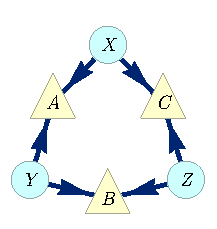
\includegraphics[scale=1]{TriDagRaw.pdf}
\caption{The causal structure of the Triangle scenario.}\label{fig:TriMainDAG}
\end{minipage}
\hfill
\begin{minipage}[t]{0.38\linewidth}
\centering
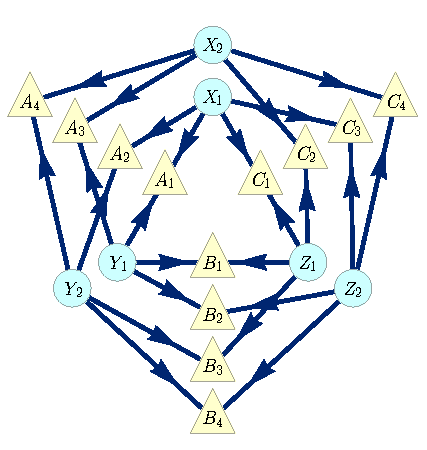
\includegraphics[scale=1]{TriDagFull222.pdf}
\caption{An inflation DAG of the Triangle scenario where each latent node has been duplicated, resulting in four copies of each observable node.}\label{fig:TriFullDouble}
\end{minipage}
\hfill
\begin{minipage}[b]{0.35\linewidth}
\centering
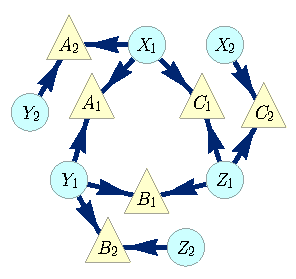
\includegraphics[scale=1]{TriDagSub222.pdf}
\caption{Another inflation of the Triangle scenario consisting, also notably $\ansubgraph[(\textrm{\cref{fig:TriFullDouble}})]{A_1 A_2 B_1 B_2 C_1 C_2}$.}\label{fig:Tri222}
\end{minipage}
\end{figure}

\begin{figure}[hb]
\centering
\begin{minipage}[t]{0.3\linewidth}
\centering
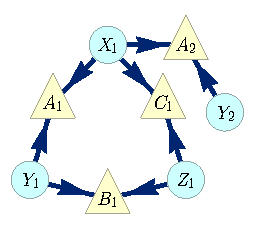
\includegraphics[scale=1]{broadcastingexamplenohighlight.pdf}
\caption{A simple inflation of the Triangle scenario, also notably $\ansubgraph[(\cref{fig:Tri222})]{A_1 A_2 B_1 C_1}$.}\label{fig:simpleinflation}
\end{minipage}\hfill
\begin{minipage}[t]{0.275\linewidth}
\centering
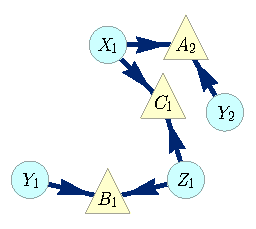
\includegraphics[scale=1]{nobroadcastingexamplenohighlight.pdf}
\caption{An even simpler inflation of the Triangle scenario, also notably $\ansubgraph[(\cref{fig:simpleinflation})]{A_2 B_1 C_1}$. }\label{fig:simplestinflation}
\end{minipage}
\hfill
\begin{minipage}[t]{0.325\linewidth}
\centering
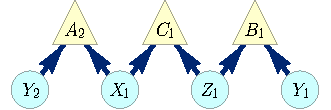
\includegraphics[scale=1]{TriDagSubA2B1C1.pdf}
\caption{Another representation of \cref{fig:simplestinflation}. Despite not containing the original scenario, this is a valid inflation per \cref{eq:definflationDAG}.}\label{fig:TriDagSubA2B1C1}
\end{minipage}
\end{figure}


Next, we turn to specifying how the parameters in the inflation of a causal model are determined from those in the original model.
%condition under which a set of parameters $\mathcal{P'}(G')$ are the inflationary image of the set of parameters $\mathcal{P}(G)$. 

The condition is simply that for every node $A_i$ in the inflation DAG $G'$, the manner in which $A_i$ depends causally on its parents within $G'$ must be the same as the manner in which $A$ depends causally on its parents within the original DAG $G$.   Formally, 
\begin{align}\label{eq:funcdependences}
%\text{If} \quad G' \in\SmallNamedFunction{Inflations}{G}\quad \text{and} \quad \mathcal{P'}(G') = \SmallNamedFunction{Inflation}{\mathcal{P}(G)} \quad \text{then}\quad \forall A_i \in \SmallNamedFunction{Nodes}{G'}:\; \pdf{A_i| \Pa[G']{A_i}}=\pdf{A|\Pa[G]{A}},
%\text{If} \quad G' \in\SmallNamedFunction{Inflations}{G}\quad \text{then} \quad C_{G'} = \SmallNamedFunction{Inflation}{C_{G}} \quad \text{iff}\quad \forall A_i \in \SmallNamedFunction{Nodes}{G'}:\; \pdf[C']{A_i| \Pa[G']{A_i}}=\pdf[C]{A|\Pa[G]{A}},
C' \in \SmallNamedFunction{Inflations}{C} \quad \text{iff}\quad G' \in\SmallNamedFunction{Inflations}{G}
%\SmallNamedFunction{DAG}{C'} \in \SmallNamedFunction{Inflations}{\SmallNamedFunction{DAG}{C}}
\quad \text{and} \quad \forall A_i \in \SmallNamedFunction{Nodes}{G'}:\; \pdf[C']{A_i| \Pa[G']{A_i}}=\pdf[C]{A|\Pa[G]{A}},
\end{align}
where Eq.~\eqref{eq:definflationDAG} guarantees that $A_i \sim A$ and $\Pa[G']{A_i} \sim \Pa[G]{A}$.  

%A causal model specifies the causal structure and the autonomous causal mechanisms.  
To sum up then, inflation is a mapping to a new causal model wherein each given variable in the original DAG may have counterparts in the inflation DAG and where the causal dependences in the inflation DAG are given by the corresponding causal dependences in the original DAG.   Note that the operation of modifying a DAG and equipping the modified version with causal dependences that mirror those of the original also appears in the \emph{do calculus} of~\citet{pearl2009causality}. \fxnote{adhesivity and non-Shannon-type ineqs}
%The copying of variables under inflation implies that causal mechanisms in the inflation DAG are not necessarily autonomous, but rather often coincide with one another.


%defines a novel sort of constraint on the parameters of a causal model.  We pause to describe this constraint in general terms, before introducing the notion of inflation.  The sorts of causal structures that can arise in our inflation scheme have the property that necessarily there will be certain pairs of variables which have the same ancestral subgraph.  The constraint on the parameters is that the two conditional probability distributions describing how each variable of the pair depends on its parents are quantitatively equal to one another.  (To our knowledge, this sort of constraint has not been considered before in causal inference.)

%The inflation DAG technique that we introduce allows questions about the viability of one causal hypothesis for certain observed data to be turned into questions about the viability of a different sort of causal hypothesis for an inflation of the observed data.

%Because we have defined inflation as a map on causal models, 
Because causal hypotheses are sets of causal models, any inflation map, by virtue of being a map on causal models, induces a map on causal hypotheses. Specifically,
\begin{align}
H_{G',S'} \in \SmallNamedFunction{Inflations}{H_{G,S}} \quad \text{iff}\quad 
\quad G' \in\SmallNamedFunction{Inflations}{G}\quad \text{and} \quad 
H_{G',S'} = \{ C' : C' = \SmallNamedFunction{Inflation}{C}, C \in H_{G,S} \}.
%\forall C' \in H_{G',S'}  \exists C \in H_{G,S} : C' = \SmallNamedFunction{Inflation}{C}.
%A_i \in \SmallNamedFunction{Nodes}{G'}:\; \pdf[C']{A_i| \Pa[G']{A_i}}=\pdf[C]{A|\Pa[G]{A}}, \SmallNamedFunction{Inflation}{H_{G,S}} = \{ \SmallNamedFunction{Inflation}{C} : C \in H_{G,S}\}
%\SmallNamedFunction{Inflation}{H_{G,S}} = \{ \SmallNamedFunction{Inflation}{C} : C \in H_{G,S}\}
\end{align}
%[Put this after the lemma] Inflation can be understood as a map over causal hypotheses as follows: An inflation map takes a causal hypothesis $H_{G,S}$  to a causal hypotheses $H_{G',S'}$, where $G'$ and $S'$ satisfy:
%\begin{itemize}
%\item The DAG $G'$ is an inflation of the DAG $G$ 
%\item $\{ \pdf{A_i| \Pa[G']{A_i}} : A_i \in \SmallNamedFunction{Nodes}{G'}\} \in S'$ if only if  $\{ \pdf{A| \Pa[G]{A}} : A \in \SmallNamedFunction{Nodes}{G}\} \in S$.
%\end{itemize}

Note that even if $S=S_{\textsf{full}}$, so that the original causal hypothesis puts no constraints on the parameter values, one generally has $S'\ne S'_{\textsf{full}}$, that is, the inflationary image of the full set of parameter values on $G$ is not the full set of parameter values on $G'$. Rather, $S'$ incorporates a nontrivial restriction on the parameters consistent with $G'$, namely, that if nodes $A_i$ and $A_j$ on $G'$ are copies of a single node $A$ on $G$,then the parameter values on $G'$ are constrained to satisfy $\pdf{A_i| \Pa[G']{A_i}}=\pdf{A_j|\Pa[G']{A_j}}$.

%Finally, we can begin to spell out how the inflation technique is useful for causal inference.  
%First, we emphasize the broad notion of causal inference that we have in mind here. 



%[Note that the distinction between observed nodes and latent nodes in the DAG $G$ is inherited by the DAG $G'$.]


To see how inflation is relevant for causal inference, we must explain how the distributions that can be achieved in the inflation model are constrained by those in the original model.  In what follows, we assume that $G' \in \SmallNamedFunction{Inflations}{G}$ and that $C' = \SmallNamedFunction{Inflation}{C}$.

Note, first of all, that for any sets of nodes $\bm{U}\in \SmallNamedFunction{Nodes}{G'}$ and   $\subsim{\bm{U}}\in \SmallNamedFunction{Nodes}{G}$,
\begin{align}\label{eq:coincidingdistrodef}
\text{if }\quad \ansubgraph[G']{\bm{U}}\sim\ansubgraph[G]{\subsim{\bm{U}}}\quad\text{then}\quad \pdf[C']{\bm{U}}=\pdf[C]{\subsim{\bm{U}}}.
\end{align}
This follows from the fact that the probability distributions over $\bm{U}$ and $\subsim{\bm{U}}$ depend only on their ancestral subgraphs and the parameters defined thereon, which by the definition of inflation are the same for $\bm{U}$ and for $\subsim{\bm{U}}$.

It is useful to have a name for a set of nodes in the inflation DAG, $\bm{U} \subseteq \SmallNamedFunction{Nodes}{G'}$, such that one can find a corresponding set in the original DAG, $\subsim{\bm{U}} \subseteq \SmallNamedFunction{Nodes}{G}$, which has an equivalent ancestral subgraph.   We say that such subsets of the nodes of $G'$ are injectable into $G$ and we call them the \tblue{injectable sets},
% into $\SmallNamedFunction{Nodes}{G}$,
\begin{align}\label{eq:definjectable}
\bm{U}\in\SmallNamedFunction{InjectableSets}{G'} \quad\text{ iff }\quad \exists \subsim{\bm{U}}\subseteq \SmallNamedFunction{Nodes}{G}: \ansubgraph[G']{\bm{U}}\sim\ansubgraph[G]{\subsim{\bm{U}}}.
\end{align}
In \cref{fig:Tri222}, for example, the set $\brackets{A_1 B_1 C_1}$ is injectable because its ancestral subgraph is equivalent up to copy-indices to the ancestral subgraph of $\brackets{A B C}$ in the original DAG (which is just the full DAG), and the set $\brackets{A_2 C_1}$ is injectable because its ancestral subgraph is equivalent to that of $\brackets{ A C}$ in the original DAG. 

Note that it is clear that a set of nodes in the inflation DAG can only be injectable if it contains at most one copy of any node from the original DAG.  Similarly, it can only be injectable if its ancestral subgraph also contains at most one copy of any node from the original DAG.  
Thus, in \cref{fig:Tri222}, $\brackets{A_1 A_2 C_1}$ is not injectable because it contains two copies of $A$, and $\brackets{A_2 B_1 C_1}$ is not injectable because its ancestral subgraph contains two copies of $Y$. 

%The relation between nodes of the inflation DAG $G'$ to nodes on the DAG $G$ that will be of primary interest to us is not injectability  actually slightly weaker than the notion of injectability.  
The sets of nodes of $G'$ that will be of primary interest to us are not the injectable sets per se, but sets satisfying a slightly weaker constraint.
%We call this notion {\em pre-injectability}.  
To define the latter sorts of sets, which we term {\em pre-injectable}, we must first introduce some additional terminology. 

We refer to a pair of nodes which do not share any common ancestor as being \tblue{ancestrally independent}, for which we invent the notation $X\aindep Y$. Generalizing to sets, $\bm{U}\aindep \bm{V}$ indicates that no node in $\bm{U}$ shares a common ancestor with any node in $\bm{V}$, 
\begin{align}
\bm{U}\aindep \bm{V} \quad \text{iff} \quad \An{\bm{U}}\cap\An{\bm{V}}=\emptyset.
\end{align}
%i.e.~$\An{\bm{U}}\cap\An{\bm{V}}=\emptyset$. 
%It is possible for more than two sets to be ancestrally independent: the notation ${\bm{U}\aindep \bm{V}\aindep \bm{W}}$ should be understood as indicating that the ancestors of $\bm{U}$,$\bm{V}$, and $\bm{W}$ comprise three distinct non-overlapping sets, i.e.~$\bm{U}\aindep \bm{V}$ and $\bm{V}\aindep \bm{W}$ and $\bm{U}\aindep \bm{W}$.
Ancestral independence is equivalent to $d$-separation by the empty set~\cite{pearl2009causality,spirtes2011causation,studeny2005probabilistic,koller2009probabilistic}. 


A set of nodes $\bm{U}$ in the inflation DAG $G'$ will be called \tblue{pre-injectable} whenever it is a union of injectable sets with disjoint ancestries. 
\begin{align}\label{eq:defpreinj}
\bm{U}\in\SmallNamedFunction{PreInjectableSets}{G'} \quad\text{ iff }\quad  \exists \{ \bm{U}_i \in \SmallNamedFunction{InjectableSets}{G'} \} \quad \text{s.t.}\quad \bm{U}=\bigcup_i \bm{U}_i  \quad\text{and} \quad  \forall i\ne j: \bm{U}_i \aindep \bm{U}_j.
%\bm{U}\in\SmallNamedFunction{PreInjectableSets}{G'} \quad\text{ iff }\quad  \exists \{ \bm{U}_i \}_i \quad \text{s.t.}\quad \bm{U}=\bigcup_i \bm{U}_i  \quad\text{and} \quad \forall i 
%: \bm{U}_i \in \SmallNamedFunction{InjectableSets}{G'}\quad \text{and}\quad \forall i,j
%: \bm{U}_i \aindep \bm{U}_j.
\end{align}
%Equivalently, a set of nodes is pre-injectable if and only if its (weakly) connected components are injectable. 
Note that every injectable set is a trivial example of a pre-injectable set.

Because ancestral independence in the DAG implies statistical independence for any probability distribution consistent with the DAG, it follows that  if 
$\bm{U}$ is a pre-injectable set and $\bm{U}_1,\bm{U}_2,\ldots,\bm{U}_n$ are the ancestrally independent components of $\bm{U}$, then 
\begin{align}%\label{eq:preinjfactor}
%\forall \bm{U}\in\SmallNamedFunction{PreInjectableSets}{G'}:	
\pdf[C']{\bm{U}} = \pdf[C']{\bm{U}_1} \pdf[C']{\bm{U}_2}  \cdots \pdf[C']{\bm{U}_n}.
\end{align}
Furthermore, because each injectable set of variables $\bm{U}_i$ satisfies Eq.~\eqref{eq:coincidingdistrodef}, it follows that joint distributions on pre-injectable sets in the inflation model can be expressed in terms of distributions defined on the original causal model,
\begin{align}\label{eq:preinjfactor}
%\forall \bm{U}\in\SmallNamedFunction{PreInjectableSets}{G'}:	
\pdf[C']{\bm{U}} = \pdf[C]{\subsim{\bm{U}}_1} \pdf[C]{\subsim{\bm{U}}_2}  \cdots \pdf[C]{\subsim{\bm{U}}_n}.
\end{align}
This latter property implies that the probability distribution over any pre-injectable set in the inflation model is fully determined by the parameters in the original causal model.  Indeed, this relation is what motivates us to consider the pre-injectable sets.

Consider a causal inference problem where the observational input is a probability distribution over a set $\bm{O}$ of observed variables, denoted $\pdf{\bm{O}}$ and the causal hypothesis is $H_{G,S}$ where $\SmallNamedFunction{ObservedNodes}{G}=\bm{O}$.  Suppose that one seeks only to determine whether the causal hypothesis is consistent with the observational input.  
%Then the following condition is necessary and sufficient for such consistency
This holds if and only if
\begin{align}
\exists C \in H_{G,S} : \pdf[C]{\SmallNamedFunction{ObservedNodes}{G}}= \pdf{\bm{O}}.
\end{align}

%Consider a causal inference problem where the input data is a joint distribution over a set of observed variables.  A causal model is only a candidate for a causal explanation of this joint distribution if it posits a DAG $G$ for which $\SmallNamedFunction{ObservedNodes}{G}$ corresponds to the set of observed variables, so we assume this henceforth. The causal hypothesis $H_{G,S}$ is consistent with data $\pdf{\SmallNamedFunction{ObservedNodes}{G}}$ if and only if there exists a causal model satisfying the constraints of the hypothesis, $C \in H_{G,S}$, such that $\pdf[C]{\SmallNamedFunction{ObservedNodes}{G}} = \pdf{\SmallNamedFunction{ObservedNodes}{G}}$. 



%Suppose the original causal inference problem takes as its inputs  a probability distribution over a set $\bm{O}$ of observed variables, denoted $\pdf{\bm{O}}$, and a causal hypothesis, denoted $H_{G,S}$, and seeks to determine whether these are consistent.  

Every inflation $G\to G'$
%DAG $G' \in \SmallNamedFunction{Inflations}{G}$
 defines a new causal inference problem for which the decision regarding consistency is the same as for the original problem.  

The causal hypothesis of the new causal inference problem is simply the image under a $G\to G'$ inflation of the causal hypothesis of the original causal inference problem, and one seeks to evaluate its consistency with observational data that is determined by the observational data of the original in the following way.
%: for all pre-injectable sets on $G'$ consisting entirely of observed nodes on $G'$, the distribution over the set is given by the observed distribution over the corresponding nodes on $G$. 

%We can formalize this as follows. 
Let  $\bm{O}$ denote the image of $\subsim{\bm{O}}$ under the $G \to G'$ inflation, and consider the subsets of $\bm{O}$ that are pre-injectable relative to the $G \to G'$ inflation, denoted $\SmallNamedFunction{PreInjectableSets}{\bm{O}}$.  Recall that for every set of nodes $\bm{U} \in \SmallNamedFunction{PreInjectableSets}{\bm{O}}$ there is a partition $\bm{U} = \bigcup_i \bm{U}_i$ where the $\bm{U}_i$ are subsets of $\bm{O}$ that are injectable relative to the $G \to G'$ inflation and that are ancestrally independent.  Recall also that, by the definition of a $G\to G'$ inflation, for any set of nodes $\bm{U}_i \subseteq \bm{O}$ that is injectable, one can find a set of nodes $\subsim{\bm{U}}_i \subseteq \subsim{\bm{O}}$ such that $\forall  i: \bm{U}_i \sim \subsim{\bm{U}}_i$.  The observational data of the new causal inference problem is that $\forall \bm{U} \in \SmallNamedFunction{PreInjectableSets}{\bm{O}}: \pdf{\bm{U}} = \pdf{\subsim{\bm{U}_1}}\pdf{\subsim{\bm{U}_2}} \dots \pdf{\subsim{\bm{U}_n}}$, where $\pdf{\subsim{\bm{U}_i}}$ is the marginal of $\pdf{\subsim{\bm{O}}}$ on $\subsim{\bm{U}_i}$.

Therefore the observational input to the new causal inference problem is not the distribution on $\bm{O}$, but rather a specification of the marginals of this distribution on each of the pre-injectable sets of $\bm{O}$ under the $G\to G'$ inflation.

Summarizing, we have:
\begin{lemma}
The causal hypothesis $H_{G,S}$ is consistent with the observational data $\pdf{\subsim{\bm{O}}}$ if and only if the image of this causal hypothesis under a $G\to G'$ inflation, denoted $H_{G',S'}$, is consistent with the observational data that $\forall \bm{U} \in \SmallNamedFunction{PreInjectableSets}{\bm{O}}: \pdf{\bm{U}} = \pdf{\subsim{\bm{U}_1}}\pdf{\subsim{\bm{U}_2}} \dots \pdf{\subsim{\bm{U}_n}}$.
\end{lemma}

It follows that any consistency conditions that one can derive for the new causal inference problem immediately yield consistency conditions for the original causal inference problem.  Indeed, any standard tool of causal inference can be applied to the new problem and conditions derived therefrom provide novel conditions for the original problem.  Any causal inference tool, therefore, can potentially have its power augmented by combining it with inflation.
%The new problem has a rather different form than the old, 



\example{: \tred{Perfect correlation cannot arise from the Triangle scenario.}}\par\smallskip\nobreak

Consider the following causal inference problem.  The observational data is a joint distribution over three binary-outcome variables, $P\parenths{A B C}$, where the marginal on each variable is uniform and the three are perfectly correlated,
\begin{align}\label{eq:ghzdistribution1}
p\parens{a b c}=\frac{[000]+[111]}{2}=\begin{cases}\tfrac{1}{2}&\text{if }\; a=b=c, \\ 0&\text{otherwise}.\end{cases}
\end{align}
The causal hypothesis is the set of causal models associated to the DAG of the triangle scenario, depicted in \cref{fig:Tri222}.  The problem is to decide whether the observational data is consistent with this causal hypothesis.

To solve this problem, we consider the causal inference problem induced by the particular inflation of the triangle scenario depicted in Fig.~\ref{fig:TriDagSubA2B1C1}.  

The sets $\brackets{A_2 C_1}$ and $\brackets{B_1 C_1}$ are injectable (hence trivially pre-injectable). The set $\brackets{A_2 B_1}$ is also pre-injectable because the singleton sets $\brackets{A_2}$ and $\brackets{ B_1}$ are each injectable and ancestrally independent.  Therefore, the observational data in our new causal inference problem includes
\begin{align}
\pdf{A_2 C_1}=\pdf{A C}\label{j1}\\
\pdf{B_1 C_1}=\pdf{B C}\label{j2}\\
\pdf{A_2 B_1}=\pdf{A}\pdf{B}\label{j3}.
\end{align}
The question is whether such constraints are consistent with the causal hypothesis that the DAG is that of \cref{fig:TriDagSubA2B1C1}, where the parameters supplementing the DAG are arbitrary, except for the constraint that the latent variables $Y_1$ and $Y_2$ are identically distributed. 

It is not difficult to see that the answer to the question is negative.  And this verdict can be rendered without even appealing to the form of the inflation DAG (Note, however, that the inflation DAG has played a role in defining the new causal inference problem insofar as it has dictated the form that the observational data should take).  It suffices to make use of results concerning the marginals problem.   From Eq.~\eqref{eq:ghzdistribution1} one deduces that the marginal $\pdf{A C}$ described perfect correlation between $A$ and $C$ and similarly for the marginal $\pdf{B C}$.  But then, by Eqs.~\eqref{j1} and \eqref{j2}, one deduces that there is perfect correlation between $A_2$ and $C_1$ and perfect correlation between $B_1$ and $C_1$.  Meanwhile, Eq.~\eqref{j3} dictates that $A_2$ and $B_1$ should be uncorrelated.  But there is no joint distribution $P(A_2 B_1 C_1)$ having such marginals:  the only joint distribution that exhibits perfect correlation between $A_2$ and $C_1$ and between $B_1$ and $C_1$ also exhibits perfect correlation between $A_2$ and $B_1$.  

We have therefore certified that perfect correlations among $A$, $B$ and $C$ is not consistent with the Triangle causal structure, recovering the seminal result of \citet{steudel2010ancestors}.

\begin{comment}
Let us ask, is it possible for the three original-scenario observable variables $\{A,B,C\}$ to be random but perfectly correlated? We call this the GHZ-type distribution, after an eponymous tripartite entangled quantum state \cite{greenberger1989going,3Qubits2Ways}. So $P_{\text{GHZ}}\parenths{A B C}$ is given by
\begin{align}\label{eq:ghzdistribution1}
p_{\text{GHZ}}\parens{a b c}=\frac{[000]+[111]}{2}=\begin{cases}\tfrac{1}{2}&\text{if }\; a=b=c, \\ 0&\text{otherwise}.\end{cases}
\end{align}
We assume uniform binary variables for the sake of concreteness, but the argument is general. Let's temporarily (falsely) assume $P_{\text{GHZ}}$ to be feasible for the triangle scenario. Since $\brackets{A_2 C_1}$ is an injectable set we have $\pdf{A_2 C_1}=\pdf{A C}$, and therefore $P_{\text{GHZ}}$ implies that $A_2$ and $C_1$ are perfectly correlated. Similarly, since $\brackets{B_1 C_1}$ is an injectable set we have $\pdf{B_1 C_1}=\pdf{A C}$, and therefore $B_1$ and $C_1$ must be perfectly correlated, and by extension $B_1$ and $A_2$ are perfectly correlated as well. On the other hand, $A_2$ and $B_1$ must be statistically independent, as they do not share any common ancestor. The only way for two variables to be \emph{both} perfectly correlated and independent is by being deterministic. This is not the case in $P_{\text{GHZ}}$, and thus we have certified that $P_{\text{GHZ}}$ is not realizable from the Triangle causal structure, recovering the seminal result of \citet{steudel2010ancestors}.
\end{comment}

\example{: \tred{The W-type distribution cannot arise from the Triangle scenario}}\par\smallskip\nobreak

Consider another causal inference problem concerning the triangle scenario, namely, that of determining whether the triangle DAG can explain a joint distribution $P_{\text{W}}\parenths{A B C}$ of the form
\begin{align}\label{eq:wdistribution1}
p_{\text{W}}\parens{a b c}=\frac{[100]+[010]+[001]}{3}=\begin{cases}\tfrac{1}{3}&\text{if }\; a+b+c=1, \\ 0&\text{otherwise}.\end{cases}
\end{align}
We call this the W-type distribution\footnote{Because its correlations are reminiscent of those one obtains for the quantum state appearing in Ref. \cite{3Qubits2Ways}, and which is called the W state.}. To our knowledge, the fact that the Triangle causal structure is inconsistent with the W-type distribution has not been demonstrated previously.

To prove the inconsistency of  $P_{\text{W}}$ with the Triangle causal structure, we consider the inflation DAG of \cref{fig:Tri222}. 
The sets $\{A_2 C_1\}$, $\{B_2 A_1\}$, $\{A_2 B_1\}$ and $\{ A_1 B_1 C_1\}$ are injectable.  The set $\{ A_2 B_2 C_2\}$ is pre-injectable because the singleton sets $\{A_2\}$,  $\{B_2\}$ and $\{C_2\}$ are injectable and acenstrally independent. It follows that we must consider the feasability of the observational data
\begin{align}
\pdf{A_2 C_1}=\pdf{A C}\label{W1}\\
\pdf{B_2 A_1}=\pdf{B A}\label{W2}\\
\pdf{C_2 B_1}=\pdf{C B}\label{W3}\\
\pdf{A_1 B_1 C_1}=\pdf{A B C}\label{W4}\\
\pdf{A_2 B_2 C_2}=\pdf{A}\pdf{B}\pdf{C}\label{W5}.
\end{align}
Eq.~\eqref{W1} together with the form of $P_{\text{W}}$ implies that $C_1\eql 0$ whenever $A_2 \eql 1$. Similarly, $A_1\eql 0$ whenever $B_2\eql 1$ and $B_1\eql 0$ whenever $C_2\eql 1$. Eq.~\eqref{W5} and the form of $P_{\text{W}}$ implies that $A_2$,$B_2$, and $C_2$ are uncorrelated and uniformly distributed, which means that sometimes they all take the value 1. 
%, that is, $A_2=1$ and $B_2=1$ and $C_2=1$.  
Summarizing, we have
\begin{align} 
A_2 \eql 1 \implies C_1\eql 0\\
B_2\eql 1 \implies A_1\eql 0\\
C_2 \eql 1 \implies B_1 \eql 0\\
\text{sometimes}
%\footnote{In fact, this occurs with probability 1/8, though it is sufficient for the argument to note that it is nonzero.}
 \quad A_2=1, B_2=1, C_2=1.
\end{align}
But these constraints clearly imply that
\begin{align}
\text{sometimes} \quad A_1=0, B_1=0, C_1=0,
\end{align}
which contradicts Eq.~\eqref{W4} and the fact that $P_{\text{W}}$ has no weight on $[000]$.

Again, we have reached our verdict here simply by noting that the distributions defined in Eqs.~\eqref{W1}-\eqref{W5} cannot arise as the marginals of a single distribution on $A_1, B_1, C_1, A_2, B_2, C_2$.  Specifically, we have leveraged an approach to the marginal problem inspired by Hardy's version of Bell's theorem [citation].

%$\p{A_2\eql B_2\eql C_2\eql 1}=\nicefrac{1}{8}$ according to $P_{\text{W}}$. But that would imply $\p{A_1\eql B_1\eql C_1\eql 0}\geq\nicefrac{1}{8}$, which contradicts $P_{\text{W}}$, hence $P_{\text{W}}$ cannot arise from the Triangle scenario.

The W-type distribution is difficult to witness as unrealizable using conventional causal inference techniques.
\begin{compactenum}
\item There are no conditional independence relations between the observable nodes of the Triangle scenario. %, so the distribution is observationally Markov with respect to the DAG. 
\item Shannon-type entropic inequalities cannot detect this distribution as not allowed by the Triangle scenario~\cite{fritz2013marginal,chaves2014novel,chaves2014informationinference}. 
\item Moreover, \emph{no} entropic inequality can witness the W-type distribution as unrealizable. \citet{weilenmann2016entropic} have constructed an inner approximation to the entropic cone of the Triangle causal structure, and the W-distribution lies inside this. In other words, a distribution with the same entropic profile as the W-type distribution \emph{can} arise from the Triangle scenario.
\item The newly-developed method of covariance matrix causal inference due to \citet{kela2016covariance}, which gives tighter constraints than entropic inequalities for the Triangle scenario, also cannot detect inconsistency with the W-type distribution.
\end{compactenum}
\par\noindent But the inflation technique can, and does so very easily.

\example{: \tred{The PR-box cannot arise from the Bell scenario}}\par\smallskip\nobreak

Consider the causal structure associated to the Bell \cite{bell1964einstein,Brunner2013Bell,bell1966lhvm,CHSHOriginal} scenario [\citealp{pusey2014gdag}~(Fig.~E\#2), \citealp{WoodSpekkens}~(Fig.~19), \citealp{chaves2014novel}~(Fig.~1), \citealp{BeyondBellII}~(Fig.~1), \citealp{wolfe2015nonconvexity}~(Fig.~2b), \citealp{steeg2011relaxation}~(Fig.~2)], depicted here in \cref{fig:NewBellDAG1}. The observable variables are $\brackets{A,B,X,Y}$, and $\Lambda$ is the latent common cause of $A$ and $B$. 

\begin{figure}[ht]
\centering
\begin{minipage}[t]{0.45\linewidth}
\centering
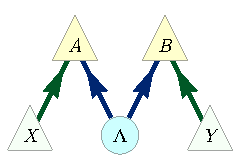
\includegraphics[scale=1]{BellDagRaw.pdf}
\caption{The causal structure of the a bipartite Bell scenario. The local outcomes of Alice's and Bob's experimental probing is assumed to be a function of some latent common cause, in addition to their independent local experimental settings.}\label{fig:NewBellDAG1}
\end{minipage}
\hfill
\begin{minipage}[t]{0.45\linewidth}
\centering
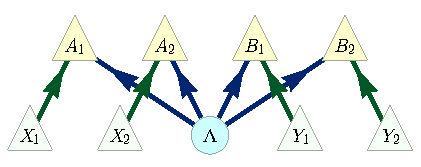
\includegraphics[scale=1]{BellDagCopy.pdf}
\caption{An inflation DAG of the bipartite Bell scenario, where both local settings variables have been duplicated.}\label{fig:BellDagCopy1}
\end{minipage}
\end{figure}


We consider the distribution ${P_{\text{PR}}}\parenths{A B X Y} = P_{\text{PR}}\parenths{A B | X Y} P(X) P(Y)$, where $P(X)$ and $P(Y)$ are arbitrary full-support distributions\footnote{In the literature on the Bell scenario, these variables are known as ``settings''. Generally, We may think of endogenous observable variables as settings, coloring them light green in the DAG figures. Settings variables are natural candidates for conditioning on.} over the binary variables $X$ and $Y$, and
\begin{align}\begin{split}\label{eq:PRbox}
% & p_{\text{PR}}\parens{a b |x y}=\frac{[00|00]+[11|00]+[00|10]+[11|10]+[00|01]+[11|01]+[01|11]+[10|11]}{8}\\
p_{\text{PR}}\parens{a b |x y}=\begin{cases}\tfrac{1}{2}&\text{if }\; \SmallNamedFunction[2]{mod}{a+b}=x\cdot y, \\ 0&\text{otherwise}.\end{cases}
\end{split}\end{align}
The correlations described by this distribution are known as PR-box correlations after Popescu and Rohrlich, and they are well-known to be inconsistent with the the Bell scenario \cite{PROriginal,PRUnit}. Here we prove this inconsistency using the inflation technique. 

We use the inflation of the Bell DAG shown in \cref{fig:BellDagCopy1}.

We begin by recognizing that $\{A_1 B_1 X_1 Y_1\}$, $\{A_2 B_1 X_2 Y_1\}$, $\{A_1 B_2 X_1 Y_2\}$, and $\{A_2 B_2 X_2 Y_2\}$ are all injectable sets, and that $\{X_1 X_2 Y_1 Y_2\}$ is a pre-injectable set because the singleton sets $\{X_1\}$, $\{X_2\}$, $\{Y_1\}$, and $\{Y_2\}$ are all injectable and ancestrally independent of one another.  It follows that
\begin{align}
\pdf{A_1 B_1 X_1 Y_1}=\pdf{A B X Y}\label{PR1}\\
\pdf{A_2 B_1 X_2 Y_1}=\pdf{A B X Y}\label{PR2}\\
\pdf{A_1 B_2 X_1 Y_2}=\pdf{A B X Y}\label{PR3}\\
\pdf{A_2 B_2 X_2 Y_2}=\pdf{A B X Y}\label{PR4}\\
\pdf{X_1 X_2 Y_1 Y_2}=\pdf{X}\pdf{X}\pdf{Y}\pdf{Y}\label{PR5}.
\end{align}
These imply that 
\begin{align}
\pdf{A_1 B_1 |X_1 Y_1}=\pdf{A B |X Y}\label{PR1b}\\
\pdf{A_2 B_1 |X_2 Y_1}=\pdf{A B |X Y}\label{PR2b}\\
\pdf{A_1 B_2 |X_1 Y_2}=\pdf{A B |X Y}\label{PR3b}\\
\pdf{A_2 B_2 |X_2 Y_2}=\pdf{A B |X Y}\label{PR4b}.
\end{align}

Given the assumption that the distributions $P(X)$ and $P(Y)$ are full support, it follows from Eq.~\eqref{PR5} that sometimes $\{X_1, X_2, Y_1, Y_2\}=\{0, 1, 0, 1\}$.  
%$X_1$, $X_2$, $Y_1$, and $Y_2$ are all independent variables.
% $P_{\text{PR}}$ is given as a conditional distribution because $X$ and $Y$ are settings variables.
For these values, $P_{\text{PR}}$ and Eq.~\eqref{PR1b} specifies perfect correlation between $A_1$ and $B_1$.  Similarly, for these values we expect perfect correlation between $A_1$ and $B_2$, perfect correlation between $A_2$ and $B_1$, and perfect \emph{anti}correlation between $A_2$ and $B_2$. Those four requirements are not mutually compatible, however: since perfect correlation is transitive, the first three properties entail perfect correlation between $A_2$ and $B_2$. 

The mathematical structure of this proof parallels that of standard proofs of the inconsistency of PR-box correlations with the Bell structure.  Standard proofs focus on a set of variables $A_0, A_1, B_0, B_1, C_0, C_1$ where $A_0$  is the value of $A$ when $X=0$, and similarly for the others.  The fact that there must be a joint distribution over these variables can be inferred from the structure of the Bell DAG and the fact that one can assume without loss of generality that the causal dependences are deterministic (a result known as Fine's theorem \cite{FineTheorem}).  It is then sufficient to note that the marginals given by the PR-box correlations do not arise from any joint distribution.  Nonetheless, our proof is conceptually distinct insofar as the variables to which we apply the marginals problem are not conditioned on a setting value.  And we do not require Fine's theorem.  [Can we do something that couldn't be done in the standard approach?]

Many causal inference techniques can be used to derive sufficient conditions for the inconsistency of the causal hypothesis $H_{G',S'}$ with the observational data $\forall \bm{U} \in \SmallNamedFunction{PreInjectableSets}{\bm{O}}: \pdf{\bm{U}} = \pdf{\subsim{\bm{U}_1}}\pdf{\subsim{\bm{U}_2}} \dots \pdf{\subsim{\bm{U}_n}}$. We will call sets of such conditions {\em inconsistency witnesses}.  

\color{black}
\section{Example applications of the inflation technique}\label{sec:examplebaddistributions}

Here are some examples of causal infeasibility criteria for the Triangle scenario which we can derive by considering the inflation DAG of~\cref{fig:TriDagSubA2B1C1}.

For technical convenience, let us assume that all observed variables take values in $\{-1,+1\}$. By virtue of the existence of a joint distribution of $A_2$, $B_1$ and $C_1$, we can conclude~\cite{kellerer_marginal_1964,leggett_garg_1985,araujo_cycle_2013},
\[
	\langle A_2 C_1\rangle + \langle B_2 C_1 \rangle - \langle A_2 B_1 \rangle \leq 1.
\]
Thanks to the relations~\cref{W1,W2,W3,W4,W5}, we can therefore conclude that if an observable distribution is compatible with the Triangle scenario DAG, then it must satisfy
\begin{equation}
	\label{eq:polymonogamy}
	\langle A C\rangle + \langle B C\rangle \leq 1 + \langle A\rangle \langle B\rangle,
\end{equation}
which we think of as a sort of monogamy inequality: it is impossible for $C$ to be strongly correlated with both $A$ and $B$, unless $A$ and $B$ are both strongly biased.

Alternatively, we could also start with the inequality~\cite{fritz2013marginal}
\[
	I(A_2 : C_1) + I(C_1 : B_1) - I(A_2 : B_1) \leq H(B_1),	
\]
which also simply follows from the existence of a joint distribution of all variables. Again applying~\cref{W1,W2,W3,W4,W5} shows in particular that the third term vanishes, and results in
\[
	I(A : C) + I(C : B) \leq H(B) ,
\]
which is the original entropic monogamy inequality derived for the Triangle scenario in~\cite{fritz2012bell}. Our rederivation in terms of inflation is essentially the proof of~\citet{pusey2014gdag}.

%To see how this distribution is incompatible with \cref{eq:tritrivial1}, note that for three \emph{identically distributed} (but not independent) binary variables a further special case of \cref{eq:tritrivial1} is
%\begin{align*}\begin{split}
%&\hspace{-6ex}3\p{A\cramp{=}1}\leq 1+\p{A\cramp{=}1}^2+2\p{A\cramp{=}B\cramp{=}1}.
%\end{split}\end{align*}
%For the W-distribution ${\p{A\cramp{=}B\cramp{=}C\cramp{=}0}=0}$, and also ${\p{A\cramp{=}1,B\cramp{=}1}=0}$, yet ${\p{A\cramp{=}1}=\nicefrac{1}{3}}$. As ${(\nicefrac{1}{3})^3\nleq 0}$ we have proven that the W-type distribution is incompatible with the Triangle scenario.
%Earlier works have already shown that the GHZ-type distribution is incompatible with the classical Triangle scenario \cite{steudel2010ancestors,fritz2012bell,chaves2014novel}. Interestingly, however, the entropic monogamy relation $I\parens{A:B}+I\parens{A:C}\leq H\parens{A}$ which rejects the GHZ-type distribution has been shown also to hold if the hidden shared resources are non-classical, even using generalized probabilistic theories \cite[Cor. 24]{pusey2014gdag}. 


\bigskip

Slightly more involved but otherwise analogous considerations can be applied to the inflation DAG of~\cref{fig:Tri222}, where in particular we have the pre-injectable sets $\{A_1 B_1 C_1\}$, $\{A_1 B_2 C_2\}$, $\{A_2 B_1 C_2\}$ and $\{A_2 B_2 C_1\}$, resulting in the factorization relations
\begin{align}
	\pdf{A_1 B_1 C_1} &= \pdf{A B C} \\
	\pdf{A_1 B_2 C_2} &= \pdf{A B} \pdf{C} \\
	\pdf{B_1 C_2 A_2} &= \pdf{B C} \pdf{A} \\
	\pdf{C_1 A_2 B_2} &= \pdf{C A} \pdf{B}.
\end{align}
Now we can again use the existence of a joint distribution over all six observable variables, which implies e.g.~the Mermin inequality~\cite{mermin_ineq_1990},
\[
	\langle A_1 B_1 C_1 \rangle - \langle A_2 B_2 C_1 \rangle - \langle A_2 B_1 C_2 \rangle - \langle A_1 B_2 C_2 \rangle \leq 2.
\]
Applying the above factorization relations turns this into the polynomial inequality
\begin{equation}
	\label{polymermin}
	\langle A B C\rangle \leq 2 + \langle A B\rangle \langle C\rangle + \langle B C \rangle \langle A\rangle + \langle C A\rangle \langle B\rangle,
\end{equation}
which is yet another necessary condition for compatibility with the Triangle scenario causal structure, and now takes genuine three-way correlations into account.


%&\qquad
% \underbrace{\begin{array}{l}
% \p{a_1 b_2 c_2}\to \p{c_2} \p{a_1 b_2} \\
% \p{a_2 b_1 c_2}\to \p{a_2} \p{b_1 c_2} \\
% \p{a_2 b_2 c_1}\to \p{b_2} \p{a_2 c_1} \\
% \p{a_2 b_2 c_2}\to \p{a_2} \p{b_2} \p{c_2} \\
%\end{array}}_{\text{via ancestral independence}}   \quad \text{ and }\quad
%\underbrace{\begin{array}{l}
%\p{a_1 b_2} \to \p{a b} \\
%\p{a_2 c_1} \to \p{a c} \\
%\p{b_1 c_2} \to \p{b c} \\
%\p{\n{a}_1 \n{b}_1 \n{c}_1}\to \p{\n{a} \n{b} \n{c}}  \\
%\end{array}\,.}_{\text{via injectable sets}}
%\end{align}

A consequence of \cref{eq:polymermin} is that the W-type distribution per \cref{eq:wdistribution1}

%\begin{align}\label{eq:wdistribution}
%{P_{\text{W}}}\parenths{A B C} \coloneqq\quad p_{\text{W}}\parens{a b c}=\frac{[100]+[010]+[001]}{3}=\begin{cases}\tfrac{1}{3}&\text{if }\; a+b+c=1 \\ 0&\text{otherwise}\end{cases}
%\end{align}

is found to be unrealizable from the Triangle scenario, by considering the special case of \cref{eq:FritzF3} where $a\cramp{\to}1$, $b\cramp{\to}1$, $c\cramp{\to}1$. \cref{eq:FritzF3} requires the use of a broadcasting inflation, and therefore does not hold in the context of general probability theories.

%, where $a,b,c\in\brackets{0,1}$.
%The W-distribution states that the in any event in which $A,B,C$ are observed, precisely one of them will be found to equal $1$ while the other two will equal $0$. The identity of the variable which takes the value $1$ is uniformly random. In informal but intuitive notation, the W-type distribution is ${\nicefrac{1}{3}[100]+\nicefrac{1}{3}[010]+\nicefrac{1}{3}[001]}$.
%To see how this distribution is incompatible with \cref{eq:FritzF3}, note that for three \emph{identically distributed} (but not independent) binary variables a further special case of \cref{eq:FritzF3} is
%\begin{align*}\begin{split}
%&\hspace{-6ex}\p{A\cramp{=}1}^3\leq \p{A\cramp{=}B\cramp{=}C\cramp{=}0} + 3\times\p{A\cramp{=}B\cramp{=}1}\p{C\cramp{=}1}.
%\end{split}\end{align*}
%For the W-distribution ${\p{A\cramp{=}B\cramp{=}C\cramp{=}0}=0}$, and also ${\p{A\cramp{=}1,B\cramp{=}1}=0}$, yet ${\p{A\cramp{=}1}=\nicefrac{1}{3}}$. As ${(\nicefrac{1}{3})^3\nleq 0}$ we have proven that the W-type distribution is incompatible with the Triangle scenario.



\cref{sec:38ineqs} provides a list of further polynomial inequalities that we have derived for the Triangle scenario using the method developed in the following section.

\section{Deriving polynomial inequalities systematically}
\label{sec:ineqs}

We have defined causal inference as a decision problem, namely testing the consistency of some observational data with some some causal hypothesis. We've shown that this decision can be negatively answered by proxy, namely by demonstrating inconsistency of \emph{inflated} data with an \emph{inflated} hypothesis. The inflation technique can also be used to derive infeasibility criteria, however, by \tblue{deriving constraints on the pre-injectable sets}. Any such constraint is also an implicit consequence of the original hypothesis, and hence a relevant infeasibility criterion.

The ``big" problem, therefore, is rather straightforward: We seek to derive causal infeasibility criteria from the inflation hypothesis on the injectable sets. This task, however, is just a special instance of generic causal inference: Given some causal hypothesis, what can we say about how it constrains possible observable marginal distribution? Any technique for deriving causal infeasibility criteria is therefore relevant when using the inflation technique. Interestingly, weak constraints from the inflation hypothesis translate into strong constraints pursuant to the original hypothesis.

In the discussion that follows we continue to assume that the original hypothesis is nothing more than supposing the causal structure to be given by the original DAG. Furthermore we presume that the joint distribution over all original observable variables is accessible. Moreover, we limit our attention to deriving polynomial inequalities in terms of probabilities. The potential of using inflation as tool for deriving entropic inequalities is considered separately in \purp{Appendix? Separate work?}

In what follows \purp{the appendices?} we consider three different strategies for constraining possible marginal distributions from the inflation hypothesis. The first strategy attempts to leverage many different kinds of constraints which are implicit in the inflation hypothesis. This strategy yields the strongest infeasibility criteria, but relies on computationally-difficult nonlinear quantifier elimination. The second strategy asks only if the various marginal distributions are compatible with \emph{any} joint distribution, without regard to the specific causal structure of the inflation DAG whatsoever. Solving the marginal problem amounts to a special linear quantifier elimination computation, one which can be  computed efficiently using Fourier-Cernikov elimination. The resulting infeasibility criteria are nevertheless still polynomial inequalities. The third strategy is based on probabilistic Hardy-type paradoxes, which we connect to the hypergraph transversal problem. This strategy requires the least computational effort, but is limited in that in only yields polynomial inequalities of a very particular form.

Preliminary to every strategy, however, is the identification of the pre-injectable sets.


\topic{\tred{Identifying the Pre-Injectable Sets}}\label{step:findpreinjectable}

To identify the pre-injectable sets, we first identify the injectable sets. To this end, it is useful to construct an auxiliary graph from the inflation DAG. Let the nodes of these auxiliary graphs be the observable nodes in the inflation DAG. The \tblue{injection graph}, then, is the undirected graph in which a pair of nodes $A_i$ and $B_j$ are adjacent if  $\An{A_i B_j}$ is irredundant. The injectable sets are then precisely the cliques\footnote{A clique is a set of nodes such that every single node is connected to every other.} in this graph, per \cref{eq:definjectable}. 

Determining the pre-injectable sets from there can be done via constructing another graph that we call the \tblue{independence graph}. Its nodes are the injectable sets, and we connect two of these by an edge if their ancestral subgraphs are disjoint. Then by definition, the pre-injectable sets can be obtained as the cliques in this graph. Taking the union of all the injectable sets in such a clique results in a pre-injectable set. Since it is sufficient to only consider the maximal pre-injectable sets, one can eliminate all those pre-injectable sets that are contained in other ones, as a final step.

Let us also define the \tblue{ancestral dependence graph}, in which two nodes are adjacent if they share a common ancestor, and its complement the \tblue{ancestral independence graph}, in the ancestrally independent nodes are adjacent. To ascertain the factorization of a node set $\bm{U}$ into ancestrally-independent partitions one considers the subgraph on  $\bm{U}$ of the ancestral dependence graph: the ancestrally-independent partitions are identically the distinct connected components of that subgraph. By examining the injection graph and the ancestral dependence graph, therefore, one is able to quickly determine all injectable sets and all ancestral independence relations.

%It is also useful to define another auxiliary graph, the \tblue{pre-injection graph} in which a pair of nodes $A_i$ and $B_j$ are connected if either $\An{A_i B_j}$ or if $A_i\aindep B_j$. The pre-injection graph is identically the union of the injection graph with the ancestral independence graph. Any clique in the pre-injection graph is \emph{not} necessarily a pre-injectable set, but every pre-injectable set must correspond to a clique in the pre-injection graph, per \cref{eq:defpreinjectable}. Moreover, maximal-size pre-injectable sets must correspond to maximal cliques in the pre-injection graph. This makes the pre-injection graph a handy tool for determining the pre-injectable sets. We start by enumerating all maximal cliques in the pre-injection graph to obtain candidate pre-injectable sets. Each candidate set is then factored into ancestrally-independent partitions by means of the ancestral dependence graph. A candidate set is a legitimately pre-injectable if and only if all of its ancestrally-independent partitions are themselves injectable. Isolating the genuine pre-injectable sets from the candidates is therefore quite easy, especially since the complete set of injectable sets is already known.

\begin{figure}[t]
\centering
\begin{minipage}[b]{0.3\linewidth}
\centering
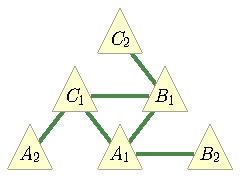
\includegraphics[scale=1]{injectiongraph222.pdf}
\caption{The auxiliary injection graph corresponding to the inflation DAG in \cref{fig:Tri222}, wherein a pair of nodes are adjacent iff they are pairwise injectable.}\label{fig:injection222}
\end{minipage}
\hfill
\begin{minipage}[b]{0.3\linewidth}
\centering
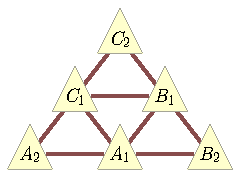
\includegraphics[scale=1]{ancestraldependancegraph222.pdf}
\caption{An auxiliary ancestral dependance graph corresponding to the inflation DAG in \cref{fig:Tri222}, wherein a pair of nodes are adjacent iff they share a common ancestor.}\label{fig:dependances222}
\end{minipage}
\hfill
\begin{minipage}[b]{0.3\linewidth}
\centering
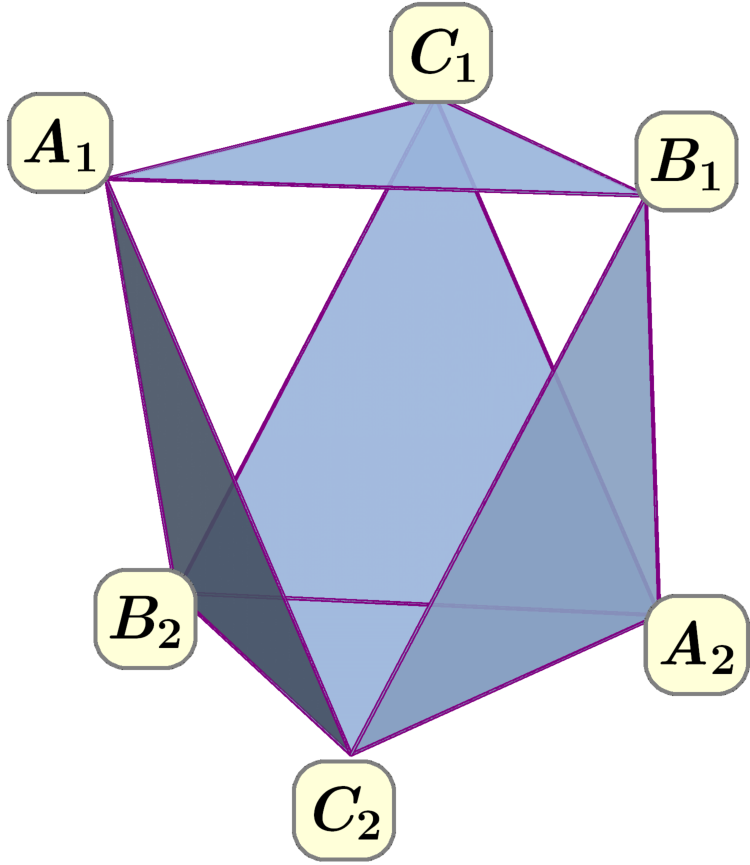
\includegraphics[scale=0.2]{simplicialcomplex.pdf}
\caption{The simplicial complex... \purp{Tobias - you please caption this?}The 5 faces in this figure correspond to the pre-injectable sets.}\label{fig:simplicialcomplex222}
\end{minipage}
\end{figure}

Applying these prescriptions to the inflation DAG in \cref{fig:Tri222} identifies the following 
 ancestral independences 
maximal injectable and maximal pre-injectable sets as follows:
\begin{align}\label{eq:basicsetup222}
{\underbrace{\begin{matrix}
A_2\aindep B_1\\
A_2\aindep C_2\\
B_2\aindep A_2\\
B_2\aindep C_1\\
C_2\aindep A_1\\
C_2\aindep B_2
\end{matrix}}_{\substack{\text{pairwise}\\\text{ancestral}\\\text{independences}}}}
\qquad\quad
{\underbrace{\begin{matrix}
\\ \\
\brackets{A_2}\aindep \brackets{B_1 B_2 C_2}\\
\brackets{B_2}\aindep \brackets{A_2 C_1 C_2}\\
\brackets{C_2}\aindep \brackets{A_1 A_2 B_2}\\
\brackets{A_2}\aindep \brackets{B_2}\aindep \brackets{C_2}
\end{matrix}}_{\substack{\text{maximal}\\\text{ancestral}\\\text{independences}}}}
\qquad\quad
{\underbrace{\begin{matrix}
\brackets{ A_1 B_1 }\\
\brackets{ B_1 C_1 }\\
\brackets{ A_1 C_1 }\\
\brackets{ A_2 C_1 }\\
\brackets{ B_2 A_1 }\\
\brackets{ C_2 B_1 }\\
\end{matrix}}_{\substack{\text{pairwise}\\\text{injectable}\\\text{sets}}}}
\qquad\quad
{\underbrace{\begin{array}{l}
\\ \\
\brackets{A_1 B_2}\\
\brackets{B_1 C_2}\\
\brackets{A_2 C_1}\\
\brackets{A_1 B_1 C_1}
\end{array}}_{\substack{\text{maximal}\\\text{injectable}\\\text{sets}}}}
\qquad\quad
{\underbrace{\begin{matrix}
\\
\brackets{A_1 B_1 C_1} \\
\brackets{A_1 B_2 C_2} \\
\brackets{A_2 B_1 C_2} \\
\brackets{A_2 B_2 C_1} \\
\brackets{A_2 B_2 C_2}
\end{matrix}}_{\substack{\text{maximal}\\\text{pre-injectable}\\\text{sets}}}}
\end{align}
such that the distributions on the pre-injectable sets relate to the original DAG distribution via
\begin{align}\label{eq:preinjectableuses222}
\begin{split}
&\forall_{a b c}:\; \p[A_1 B_1 C_1]{a b c} = \p[A B C]{a b c} \\
&\forall_{a b c}:\; \p[A_1 B_2 C_2]{a b c} = \p[C]{c}\p[A B]{a b}\\%\pdf{C}\pdf{A B}\\
&\forall_{a b c}:\; \p[A_2 B_1 C_2]{a b c} = \p[A]{a}\p[B C]{b c}\\
&\forall_{a b c}:\; \p[A_2 B_2 C_1]{a b c} = \p[B]{b}\p[A C]{a c}\\
&\forall_{a b c}:\; \p[A_2 B_2 C_2]{a b c} = \p[A]{a}\p[B]{b}\p[C]{c}
\end{split}
\end{align}
Having identified the pre-injectable sets (and how to use them), we next consider various ways to invoke constraints on the distributions over the pre-injectable sets.


\topic{\tred{Constraining Possible Distribution over Pre-Injectable Sets via the Marginal Problem}}\label{step:marginalsproblem}

The most trivial constraint on possible marginal probabilities, regardless of causal structure,  
%on the pre-injectable set
is simply the \emph{existence of some joint probability distribution} from which the marginal distributions can be recovered through marginalization, i.e. the possible marginal distributions must be \tblue{marginally compatible}. This isn't really causal inference -- as no hypothesis is considered -- but rather more of a preliminary sanity check. If the marginal distributions are not marginally compatible, then the answer to ``Can these marginal distributions be explained by this particular causal hypothesis?" is automatically ``No". 

The necessary and sufficient conditions for marginal compatibility are easy enough to state. There must exist some joint distribution (a collection of nonnegative joint probabilities) such that the marginal distributions can be recovered (each marginal distribution is a sum over various joint probabilities). \tblue{Solving the marginal problem} means resolving these "exists" statements into quantifier-free inequalities such that satisfaction of all such inequalities is necessary and sufficient for marginal compatibility. An efficient algorithm to solve the marginal problem is given in \purp{appendix... ??}. The marginal problem comes up in a variety of applications, and has been studied extensively; see~\cite{fritz2013marginal} for further references.

As an example, here's how the marginal problem would be phrased as a partial-existential-closure problem with respect to the five three-variable marginal distributions corresponding to the pre-injectable sets in \cref{eq:preinjectableuses222}.

over all the observable variables in the inflation DAG. Each of the  is a different marginal distribution of the six-variable joint distribution $\pdf{A_1 A_2 B_1 B_2 C_1 C_2}$. Solving the marginal problem means finding inequalities on the marginal distributions such that the inequalities will satisfied only if there exists some joint distribution  

From now on, one can apply \emph{any} method for dealing with the marginal problem. For example if one is given a particular distribution $P$ over the original scenario variables, then one can use~\cref{eq:preinjfactor} to compute the marginal distributions over the pre-injectable sets in an inflation DAG. Efficient linear programming can be used to to check whether there exists a joint distribution reproducing these marginals \cite{Korovin2012ImplementingCRA,Bobot2012SimplexSAT}. If such a joint distribution does not exist, then the given original-scenario distribution is witnessed as inconsistent with the original causal structure. If a joint distribution \emph{does} exist then the problem remains open, and one can try again using a different inflation.

In order to derive inequalities that hold for \emph{all} distributions that are feasible on the original DAG, say for a given number of outcomes per variable, we can formally solve the marginal problem via linear quantifier elimination, as we review in the following. This consists of eliminating unknowns from a set of linear inequalities and equalities.

The linear inequalities correspond to the nonnegativity of the joint distribution. Formally, the probability of any possible assignment of outcomes to to the observable variables is constrained to be nonnegative. For the six observable variables in \cref{fig:Tri222}, for example, the linear inequalities are given by 
\begin{align}\label{eq:nonnegativity}
\forall_{a_1 a_2 b_1 b_2 c_1 c_2}:\;0\leq \p[A_1 A_2 B_1 B_2 C_1 C_2]{a_1 a_2 b_1 b_2 c_1 c_2}
\end{align}

$0\leq \pdf{A_1 A_2 B_1 B_2 C_1 C_2}$. Note than a single inequality (or equality) pertaining to a probability \emph{distribution} is actually shorthand for a whole set of inequalities (or equalities) pertaining to the probabilities of individual events. Taking the observable variables to be binary, for example, would mean that \cref{eq:nonnegativity} would be shorthand for 64 distinct nonnegativity inequalities.
%, namely
%\begin{align}\label[eqs]{eq:nonnegativities}
%\begin{split}
% & 0\leq \p{a_1 a_2 b_1 b_2 c_1 c_2} ,\quad
% 0\leq \p{\n{a}_1 a_2 b_1 b_2 c_1 c_2} ,\quad
% 0\leq \p{a_1 \n{a}_2 b_1 b_2 c_1 c_2} ,\quad...\quad,\\
% &
% 0\leq \p{\n{a}_1 \n{a}_2 b_1 b_2 c_1 c_2} ,\quad
% 0\leq \p{\n{a}_1 a_2 \n{b}_1 b_2 c_1 c_2}, \quad ...
%\end{split}
%\end{align}
%etc. 
For a marginals problem based on the joint existence of $n$ observable variables, each ranging over $r$ possible outcomes, one would initialize the problem with $r^n$ linear nonnegativity inequalities. Unlike probabilities pertaining to injectable sets, these joint probabilities are \emph{not} fully specified by probabilities which are observed in the original scenario. We coin the term \tblue{gedankenprobability} to denote a probability pertaining to a not-pre-injectable set of inflation-DAG variables. The gedankenprobabilities evoke thought experiments, because knowing the original-scenario causal model determines the gedankenprobabilities. % \emph{in-principle}.

The linear equations in the marginal problem are those equations which express each of the marginal probabilities as a sum over various different gedankenprobabilities, namely marginalization. %Again using distribution shorthand, 
The five marginal distributions in \cref{eq:preinjectableuses222} would correspond to the equations
\begin{align}\label[eqs]{eq:marginalequalities222}
\begin{split}
&\forall_{a_1 b_1 c_1}:\;\p[A_1 B_1 C_1]{a_1 b_1 c_1} = \sum\nolimits_{a_2 b_2 b_2}\p[A_1 A_2 B_1 B_2 C_1 C_2]{a_1 a_2 b_1 b_2 c_1 c_2},\\
&\forall_{a_1 b_2 c_2}:\;\p[A_2 B_2 C_2]{a_1 b_2 c_2} = \sum\nolimits_{a_2 b_1 c_1}\p[A_1 A_2 B_1 B_2 C_1 C_2]{a_1 a_2 b_1 b_2 c_1 c_2},\\
&\forall_{a_2 b_1 c_2}:\;\p[A_2 B_1 C_2]{a_2 b_1 c_2} = \sum\nolimits_{a_1 b_2 c_1}\p[A_1 A_2 B_1 B_2 C_1 C_2]{a_1 a_2 b_1 b_2 c_1 c_2},\\
&\forall_{a_2 b_2 c_1}:\;\p[A_2 B_2 C_1]{a_2 b_2 c_1} = \sum\nolimits_{a_1 b_1 c_2}\p[A_1 A_2 B_1 B_2 C_1 C_2]{a_1 a_2 b_1 b_2 c_1 c_2},\\
&\forall_{a_2 b_2 c_2}:\;\p[A_2 B_2 C_2]{a_2 b_2 c_2} = \sum\nolimits_{a_1 b_1 c_1}\p[A_1 A_2 B_1 B_2 C_1 C_2]{a_1 a_2 b_1 b_2 c_1 c_2}.
\end{split}
\end{align}
To be clear, taking the observable variables to be binary would mean that each equality in \cref{eq:marginalequalities222} is shorthand for 8 distinct marginalization equations. 

Solving the marginal problem means eliminating all the gedankenprobabilities such as $\p[A_1 A_2 B_1 B_2 C_1 C_2]{\_\_\_\_\_\_}$ from the system of inequalities and equalities. Practically, this is accomplished by linear quantifier elimination. As an equivalent description of the same problem, but could likewise consider the problem of determining the facets of the marginal polytope, the vertices of which are known to be given by the deterministic points (compare Fine's theorem~\cite{FineTheorem} in the Bell scenario case).

Geometrically, linear quantifier elimination is equivalent to projecting a high-dimensional polytope in halfspace representation (inequalities and equalities) into a lower-dimensional quotient space.

Polytope projection is a well-understood problem in computational optimization, and a surprising variety of algorithms are available for the task \cite{jones2004equality,JonesThesis2005,Jones2008}. The oldest-known method for polytope projection, i.e. linear quantifier elimination, is an algorithm known as Fourier-Motzkin (FM) elimination \cite{fordan1999projection,DantzigEaves}, although Fourier-Cernikov elimination variant \cite{Shapot2012,Bastrakov2015}, as well as Block Elimination and Vertex Enumeration \cite{Avis2000lrs}, are also fairly popular. More advanced polytope projection algorithms, such as Equality Set Projection (ESP) and Parametric Linear Programming, have also recently become available \cite{jones2004equality,JonesThesis2005,Jones2008}. 

Linear quantifier elimination routines are available in many software tools\footnote{For example \textit{MATLAB$^{_{\textit{\tiny\texttrademark}}}$}'s \href[pdfnewwindow]{http://people.ee.ethz.ch/~mpt/2/docs/refguide/mpt/@polytope/projection.html}{\texttt{MPT2}}/\href[pdfnewwindow]{http://ellipsoids.googlecode.com/svn-history/r2740/branches/issue_119_vrozova/tbxmanager/toolboxes/mpt/3.0.14/all/mpt3-3_0_14/mpt/modules/geometry/sets/@Polyhedron/projection.m}{\texttt{MPT3}}, \textit{Maxima}'s \href[pdfnewwindow]{http://maxima.sourceforge.net/docs/manual/de/maxima_75.html}{\texttt{fourier\_elim}}, \textit{lrs}'s \href[pdfnewwindow]{http://cgm.cs.mcgill.ca/~avis/C/lrslib/USERGUIDE.html\#fourier}{\texttt{fourier}}, or \textit{Maple$^{_{\textit{\tiny\texttrademark}}}$}'s (v17+) \href[pdfnewwindow]{http://www.maplesoft.com/support/help/maple/view.aspx?path=RegularChains/SemiAlgebraicSetTools/LinearSolve}{\texttt{LinearSolve}} and \href[pdfnewwindow]{http://www.maplesoft.com/support/help/Maple/view.aspx?path=RegularChains/SemiAlgebraicSetTools/Projection}{\texttt{Projection}}. The efficiency of most of these software tools, however, drops off markedly when the dimension of the final projection is much smaller than the initial space of the inequalities. FM elimination aided by Cernikov rules \cite{Shapot2012,Bastrakov2015} is implemented in \href[pdfnewwindow]{http://sbastrakov.github.io/qskeleton/}{\textit{qskeleton}} \cite{qskeleton}. ESP  \cite{jones2004equality,JonesThesis2005,Jones2008} is supported by \href[pdfnewwindow]{http://people.ee.ethz.ch/~mpt/2/docs/refguide/mpt/@polytope/projection.html}{\texttt{MPT2}} but not \href[pdfnewwindow]{http://people.ee.ethz.ch/~mpt/3/}{\texttt{MPT3}}, and by the (undocumented) option of \href[pdfnewwindow]{https://github.com/tulip-control/polytope/blob/master/polytope/polytope.py\#L1406}{projection} in the \href[pdfnewwindow]{https://pypi.python.org/pypi/polytope}{\textit{polytope}} (v0.1.1 2015-10-26) python module.}. We have found custom-coding an linear elimination routine in \textit{Mathematica$^{_{\textit{\tiny\texttrademark}}}$} to be most efficient, see \cref{sec:projalgorithms} for further detail.
%\footnote{FM elimination algorithms make intermittent calls to a linear-programming subroutine for eliminating redundant inequalities. The authors found an efficient implementation of this subroutine in \textit{Mathematica$^{_{\textit{\tiny\texttrademark}}}$}, see \cref{sec:redundancy} for further details.}.
%Fourier-Motzkin elimination appreciable suboptimal, however, when the dimension of the final projection is much smaller than the initial space of the inequalities, i.e. when there are many gedankenprobabilities. See Refs. \cite{jones2004equality,JonesThesis2005,Jones2008} and \cref{sec:projalgorithms} for further detail.


Linear quantifier elimination is already widely used in causal inference to derive entropic inequalities \cite{fritz2013marginal,chaves2014novel,chaves2014informationinference}. In that task, however, the quantifiers being eliminated are those entropies which refer to hidden variables. By contrast, the probabilities we consider here are exclusively in terms of observable variables right from the very start. The quantifiers we eliminate are the gedankenprobabilities, which are quite different from probabilities involving hidden variables.

One may include further linear constraints beyond the usual marginals problem. For example, we know that sometimes the distributions of different injectable sets coincide, i.e. 
$\pdf{\bm{X}}=\pdf{\bm{Y}}$ whenever both $\bm{X}$ and $\bm{Y}$ are injectable, and $\subsim{\bm{X}}=\subsim{\bm{Y}}$, because injectability implies $\pdf{\bm{X}}=\pdf{\subsim{\bm{X}}}$ etc. Such equations relating coinciding marginal distributions can be used to further constrain the gedankenprobabilities; they can even be used to pre-eliminate some gedankenprobabilities through Gaussian elimination, slightly reducing the need for linear quantifier elimination. These linear constraints are not part of the usual marginal problem, however; see \cref{sec:nonlinearelimination} for further discussion.

One may also substitute numeric values for all the pre-injectable probabilities appearing in the marginals problem. Upon doing so, the quantifier elimination problem is converted to a quantifier existence problem: Do there exist gedankenprobabilities that satisfy the resulting system of inequalities? Such \emph{satisfiability} questions can be resolved quite rapidly, especially when the quantifiers are linear \cite{Korovin2012ImplementingCRA,Bobot2012SimplexSAT}. Note that real-world data with uncertainties can also be incorporated into these satisfiability questions. Instead of asserting that a particular probability is equal to a given \emph{value}, one can incorporate new inequalities which constrain the experimentally-known probabilities to lie in given \emph{intervals}. Assigning probabilities to intervals as opposed to numeric values results in further free parameters in the system, but the problem nevertheless remains one of \emph{universal} existential closure, and can be resolved with extreme efficiency.

Although linear quantifier elimination can be highly optimized, it can still prove computationally difficult. It is therefore sometimes useful to consider relaxations of the marginals problem. The \emph{full} marginals problem is to find inequalities on the marginal distributions such that the inequalities are satisfied \emph{if and only if} the given marginal distributions can be extended. It is much easier to generate necessary-but-insufficient inequalities, i.e. satisfied by all compatible marginal distributions but such that no-violation does not certify marginal compatibility. We have identified a technique for rapidly generating such quantifier-free inequalities by restricting the search to inequalities of a very particular form. We found this alternative technique — trading generality for speed — to be extraordinarily practical. The type of inequalities that we consider are given by a certain class of tautologies in classical propositional logic, see \cref{sec:TSEM} for further details.

%One useful alternative to linear quantifier elimination is to identify representative probability distributions which are incompatible with the (unprojected) constraints; \citet{ChavesNoSignalling} use this technique, for example. %That technique essentially translates the elimination problem to a satisfiability problem, and moreover an ultra-efficient \emph{linear} quantifier existence problem at that! In the context of polytope projection, these representative probability distributions correspond to extreme rays of the so-called ``projection cone" \cite{jones2004equality,Jones2008,BalasProjectionCone}.

%A final alternative to linear quantifier elimination is to restrict one's consideration to quantifier-free inequalities with a particular form. We found this alternative technique — trading generality for speed — to be extraordinarily practical. The subtype of causal criteria which can be most rapidly recognized are those which follow from certain tautologies in classical propositional logic, see \cref{sec:TSEM} for further details.




%\purp{It is interesting to compare the technique for deriving polynomial inequalities here to that in in Ref. \cite{ChavesPolynomial}. One the one hand, our initial set of linear inequalities is much stronger, as we work with the inflated DAG whereas \citet{ChavesPolynomial} considers only the original DAG. This allows us to analyze scenarios which Ref. \cite{ChavesPolynomial} cannot, namely those without any observable conditional independence relations, such as the Triangle scenario. On the other hand, Ref. \cite{ChavesPolynomial} purportedly incorporates any kind of observable conditional independence relation, whereas we account only for \emph{unconditional} independence relations, per \cref{step:fac}. A careful examination of Ref. \cite{ChavesPolynomial}, however, reveals that only unconditional independence relations are utilized in all the example there. To that extent, therefore, all the explicit results in Ref. \cite{ChavesPolynomial} are implied by the inflation DAG technique.}

%We note that our polynomial inequalities are related to those introduced recently by \citet{ChavesPolynomial}, in that our inequalities subsume the explicit results of Ref. \cite{ChavesPolynomial}. \purp{NEEDS CONFIRMATION!} \citet{ChavesPolynomial} exploits conditional independence at the observable level only, whereas our technique is applicable to scenarios even without any observable CI relations, such as the Triangle scenario.


As far as we can tell, our inequalities are not related to the nonlinear infeasibility criteria which have been derived specifically to constrain classical networks \cite{TavakoliStarNetworks,RossetNetworks,TavakoliNoncyclicNetworks}, nor to the nonlinear inequalities which account for interventions to a given causal structure \cite{kang2007polynomialconstraints,steeg2011relaxation}.




\section{Bell scenarios and inflation}

\begin{comment}


\begin{figure}[b]
\centering
\begin{minipage}[t]{0.45\linewidth}
\centering
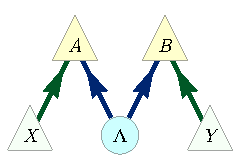
\includegraphics[scale=1]{BellDagRaw.pdf}
\caption{The causal structure of the a bipartite Bell scenario. The local outcomes of Alice's and Bob's experimental probing is assumed to be a function of some latent common cause, in addition to their independent local experimental settings.}\label{fig:NewBellDAG}
\end{minipage}
\hfill
\begin{minipage}[t]{0.45\linewidth}
\centering
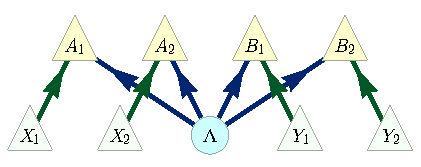
\includegraphics[scale=1]{BellDagCopy.pdf}
\caption{An inflation DAG of the bipartite Bell scenario, where both local settings variables have been duplicated.}\label{fig:BellDagCopy}
\end{minipage}
\end{figure}
\end{comment}

To further illustrate our inflation-DAG approach, we demonstrate how to recover all Bell inequalities \cite{Brunner2013Bell,bell1966lhvm,CHSHOriginal} via our method. To keep things simple we only discuss the case of a bipartite Bell scenario with two possible ``settings'' here, but the cases of more settings and/or more parties are totally analogous.
%It is critical that our method should be able to derive these seminal criteria, as Bell inequalities have been a foundational component of quantum information theory for the last half century \cite{scarani2012device,BancalDIApproach}.

Consider the causal structure associated to the Bell/CHSH \cite{bell1964einstein,Brunner2013Bell,bell1966lhvm,CHSHOriginal} experiment [\citealp{pusey2014gdag}~(Fig.~E\#2), \citealp{WoodSpekkens}~(Fig.~19), \citealp{chaves2014novel}~(Fig.~1), \citealp{BeyondBellII}~(Fig.~1), \citealp{wolfe2015nonconvexity}~(Fig.~2b), \citealp{steeg2011relaxation}~(Fig.~2)], depicted here in \cref{fig:NewBellDAG1}. The observable variables are $A,B,X,Y$, and $\Lambda$ is the latent common cause of $A$ and $B$.

In the Bell scenario DAG, one usually works with the conditional distribution $P(AB|XY)$, which is an array of distributions over $A$ and $B$ indexed by the possible values of $X$ and $Y$, instead of with the original distribution $P(ABXY)$. The maximal pre-injectable sets then are
\begin{align*}
&\brackets{A_1 B_1, X_1 X_2 Y_1 Y_2} \\
&\brackets{A_1 B_2, X_1 X_2 Y_2 Y_2} \\
&\brackets{A_2 B_1, X_1 X_2 Y_2 Y_2} \\
&\brackets{A_2 B_2, X_1 X_2 Y_2 Y_2} ,
\end{align*}
where we have put commas in order to clarify that every maximal pre-injectable set contains \emph{all} ``settings'' variables. Using these pre-injectables result in the given marginal distributions to take on the form
\begin{align*}
	P_{A_1 B_1 X_1 X_2 Y_1 Y_2}(a b x_1 x_2 y_1 y_2) & = P_{A B X Y}(a b x_1 y_1) P_X(x_2) P_Y(y_2), \\
	P_{A_1 B_2 X_1 X_2 Y_1 Y_2}(a b x_1 x_2 y_1 y_2) & = P_{A B X Y}(a b x_1 y_2) P_X(x_2) P_Y(y_1), \\
	P_{A_2 B_1 X_1 X_2 Y_1 Y_2}(a b x_1 x_2 y_1 y_2) & = P_{A B X Y}(a b x_2 y_1) P_X(x_1) P_Y(y_2), \\
	P_{A_2 B_2 X_1 X_2 Y_1 Y_2}(a b x_1 x_2 y_1 y_2) & = P_{A B X Y}(a b x_2 y_2) P_X(x_1) P_Y(y_1), \\
		P_{X_1 X_2 Y_1 Y_2}(x_1 x_2 y_1 y_2) & = P_X(x_1) P_X(x_2) P_Y(y_1) P_Y(y_2).
\end{align*}
Although the last equations follows from each of the others together with the Markov condition $P_{XY} = P_X P_Y$ for the original distribution, it nevertheless turns out to be useful to write down explicitly: putting $x_1 = y_1 = 0$ and $x_2 = y_2 = 1$ and dividing the first equation by the last one results in
\begin{align*}
	P_{A B X Y}(a b | 0 0)  =  \sum_{a',b'} P_{A_1 A_2 B_1 B_2 X_1 X_2 Y_1 Y_2}(aa'bb'|0101),
\end{align*}
and similarly also $P_{A B X Y}(a b | 0 1)$, $P_{A B X Y}(a b | 1 0)$ and $P_{A B X Y}(a b | 1 1)$ can be written as marginals of a conditional distribution. By Fine's Theorem~\cite{FineTheorem}, this implies the existence of a hidden-variable model. Conversely, if a hidden-variable model exists, then the existence of the inflation model implies the existence of a solution to the marginal problem. In conclusion, we therefore find in the case of the inflation DAG~\cref{fig:BellDagCopy1}, our method provides a necessary and sufficient condition for feasibility with the Bell causal structure. In particular, the marginal problem on this inflation DAG reproduces \emph{all} Bell inequalities.

\begin{comment}
Analysis of the inflated DAG in \cref{fig:BellDagCopy1} shows that 
\begin{align}\label{eq:bellypolymapped}
 \p{a b x y}\p{\n{x}} \p{\n{y}}
&\leq
 \p{a \n{b} x \n{y}}\p{\n{x}}\p{y} +  \p{\n{a} b \n{x} y}\p{x} \p{\n{y}}+\p{a b \n{x} \n{y}}\p{x} \p{y}
\\
\shortintertext{by virtue of the unmapped (but factored) inequality}
\label{eq:bellypolyunmapped}
 \p{a_1 b_1 x_1 y_1}\p{\n{x}_2} \p{\n{y}_2}
&\leq
 \p{a_1 \n{b}_2 x_1 \n{y}_2}\p{\n{x}_2} \p{y_1} +\p{\n{a}_2 b_1 \n{x}_2 y_1}\p{x_1}\p{\n{y}_2}+  \p{a_2 b_2 \n{x}_2 \n{y}_2}\p{x_1} \p{y_1}
\end{align}
where \emph{every} probability appearing in \cref{eq:bellypolyunmapped} maps to the original scenario, hence yielding \cref{eq:bellypolymapped}. To derive the usual Bell inequalities from \cref{eq:bellypolymapped} we switch to conditional probabilities via ${\p{a b x y}\to\p{a b | x y}\p{x y}=\p{a b | x y}\p{x}\p{y}}$ which, after dividing both sides of \cref{eq:bellypolymapped} by $\p{x}\p{\n{x}}\p{y}\p{\n{y}}$, yields
\begin{align}\label{eq:chwithneg}
&\p{a b | x y}
\leq
{\p{a \n{b} | x \n{y}} + \p{\n{a} b | \n{x} y}+\p{a b | \n{x} \n{y}}}
\\
\hspace{-\mathindent}\text{or, equivalently,}\quad
\label{eq:chwithoutneg}
&{\p{a b | x y}+\p{a b | x \n{y}} + \p{a b | \n{x} y}}
\leq
{\p{a|\n{x}}+\p{b|\n{y}} + \p{a b | \n{x} \n{y}}}
\end{align}
which is precisely the Clauser-Horne (CH) inequality \cite{CHInequality} for the Bell scenario. Note that to obtain \cref{eq:chwithoutneg} from \cref{eq:chwithneg} we implicitly made use of the no-signalling assumptions, namely $\p{a|x y}=\p{a|x}$ and $\p{b| x y}=\p{b | y}$. The CH inequality is the \emph{unique} Bell inequality (up to permutations) for the Bell scenario if $\brackets{A,B,X,Y}$ are all binary, and hence the CH inequality is a necessary and sufficient criterion to ascertain if correlations are compatible with that Bell scenario variant.

The causal structure of a Bell scenario can also be formulated directly in terms of conditional random variables. For example, the conditional-structure interpretation of \cref{fig:BellDagCopy1} is \cref{fig:BellConditionalDAG}. 

\begin{figure}[t]
\centering
\begin{minipage}[t]{0.45\linewidth}
\centering
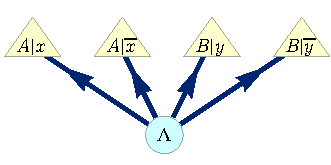
\includegraphics[scale=1]{BellDagConditionForm.pdf}
\caption{The causal structure of the Bell scenario expressed in a form which makes use of conditional random variables.}\label{fig:BellConditionalDAG}
\end{minipage}
%\hfill
%\begin{minipage}[t]{0.45\linewidth}
%\centering
%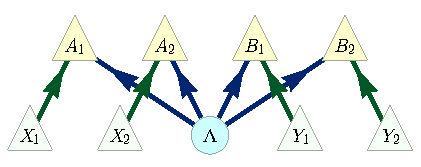
\includegraphics[scale=1]{BellDagCopy.pdf}
%\caption{An inflation DAG of the Bell scenario, where both local settings variables have been duplicated.}\label{fig:BellDagCopy}
%\end{minipage}
\end{figure}

The Bell inequalities are then self-evident from \cref{fig:BellConditionalDAG} without the need for an inflation DAG. The conditional-structure formulation innately implies its own inaccessible gedankenprobabilities, such as $\{\p{a|x , a|\n{x}}$, $\p{a|x , \n{a}|\n{x}},...\}$ etc. By eliminating these gedankenprobabilities from the set of inequalities generated by $0\leq \pdf{A|x , A|\n{x} , B|y , B|\n{y}}$ we obtain
\begin{align}\label{eq:bellcondeq}
0
\leq
{\p{a|\n{x}} + \p{b|\n{y}} + \p{a|x , b|y} -\p{a|x ,b|\n{y}} -\p{a|\n{x} , b|y} -\p{a|\n{x} , b|\n{y}}}\,,
\end{align}
for example. It should be clear that \cref{eq:bellcondeq} is equivalent to \cref{eq:chwithoutneg}.

%We can perform quantifier elimination on the set of (polynomial) inequalities given by $0\leq \pdf{A|x , A|\n{x} , B|y , B|\n{y}}$. The use of a conditional-structure DAG innately implies certain inaccessible gedankenprobabilities, such as $\{\p{a|x , a|\n{x}}$, $\p{a|x , \n{a}|\n{x}},...\}$ etc. 
\purp{Rob says kill next two paragraphs?}

Conditional-structure gedankenprobabilities are somewhat different from the inflation DAG kind, in that they reference multiple counterfactual events, such as ``What is the probability that Alice would choose to visit the museum \emph{IF} (given that) it's a rainy day in Maryland \emph{AND} that Alice would choose to go the beach \emph{IF} (given that) it's sunny in Maryland?". By contrast, unconditional gedankenprobabilities which live on an inflation DAG reference multiple heterofactual (for lack of a better word) events, such as ``What is the probability that Alice-copy-\#1 chooses to visit the museum \emph{AND} that it's raining in Maryland-copy-\#1 \emph{AND} that Alice-copy-\#2 chooses to go the beach \emph{AND} that it's sunny in Maryland-copy-\#2?". 

Joint counterfactual probabilities are experimentally inaccessible, just the same as joint heterofactual probabilities are. Suppose one could establish both Alice's propensity for going to the museum when it rains and her propensity for going to the beach when it's sunny. Even so, neither the joint counterfactual probability nor the joint heterofactual probability can be established from that limited data. For example, the value of the hidden variable ${\Lambda\cramp{=}\lambda}$ may influence Alice's willingness to get out of bed at all, or determine if she is on-call as a volunteer EMT on a particular day, or $\lambda$ might encode if Alice is travelling out-of-state. If we could measure $\p{a|x , \n{a}|\n{x}},...\}$ we might learn that Alice's likelihood of visiting the museum if it rains in Maryland is highly correlated with her likelihood of visiting the beach when it's sunny in Maryland. Or we might learn that those two counterfactual probabilities are relatively statistically independent. The ``hidden-ness" of the classical variable corresponding to the latent node shields the gedankenprobabilities from being determined. 
\end{comment}

\section{Gedankenprobabilities and the Quantum No-Broadcasting Theorem}\label{sec:classicallity}

It is worth noting that duplicating an outgoing edge in a causal structure means \tblue{broadcasting} the value of the random variable. For example in \cref{fig:simpleinflation}, the information about $X$ which was ``sent" to $A$ is effectively broadcast to both $A_1$ and $A_2$ in the inflation. This is quite intentional. Quantum theory is governed by a no-broadcasting theorem \cite{NoCloningQuantum1996,NoCloningGeneral2006}; by electing to embed broadcasting into an inflation DAG we can specifically construct a foil to quantum causal structures. Infeasibility constraints derived from \tblue{non-broadcasting inflations} on the other hand, such as \cref{fig:simplestinflation}, are valid even when relaxing the interpretation of latent nodes to allow for quantum or general probabilistic resources. This contrast is elaborated at length in \cref{sec:classicallity}.  

So a non-broadcasting inflation DAG is one in which the set of children of every latent node in the inflation DAG $G'$ is irredundant, i.e.  
\begin{align}\label{eq:nonbroadcastinginflationDAG}
G'\in\SmallNamedFunction{NonBroadcastingInflations}{G} \quad\text{ iff }\quad \forall_{\text{latent }A_i\in G'}\; \Ch[G']{A_i} \text{ is an irredundant set.}
\end{align}
We also find it useful to define the notion of a non-broadcasting subset of nodes within some larger broadcasting inflation DAG.
Let's define any pair of redundant nodes which share a latent parent to be a \tblue{fundamental broadcasting pair}. An inflation DAG is non-broadcasting if it does not contain any fundamental broadcasting pairs. Similarly, a set of nodes $\bm{U}$ is a \tblue{non-broadcasting set} iff $\An[G']{\bm{U}}$ is free of any fundamental broadcasting pairs.

%A set of nodes $\bm{U}$ is a \tblue{non-broadcasting set} iff $\ansubgraph[G']{\bm{U}}$ is a non-broadcasting inflation DAG. Any inference about the original DAG which can be made by referencing exclusively to non-broadcasting sets hold in both the classical and quantum paradigms. Broadcasting inflation DAGs are therefore especially useful for deriving criteria which distinguish quantum and classical probability distributions, but we anticipate them to be valuable for broader causal inference tasks as well.

In classical causal structures the latent nodes correspond to classical hidden variables. In quantum causal structures, however, the latent nodes are taken to be quantum systems. Some quantum causal structures are famously capable of realizing distributions that would not be possible classically, although the set of quantum distribution is superficially quite similar to the classical subset \cite{pusey2014gdag,fritz2012bell}. For example, classical and quantums distributions alike respect all conditional independence relations implied by the common underlying causal structure \cite{pusey2014gdag}. Recent work has found that quantum causal structure implies many of the entropic inequalities implied by their classical counterparts \cite{pusey2014gdag,Chaves2015infoquantum,ChavesNoSignalling}. To-date, no quantum distribution has been witnessed to violate a Shannon-type entropic inequality on observable variables derived from the Markov conditions on all nodes \cite{chaves2012entropic,fritz2012bell}. Fine-graining the scenario by conditioning on discrete settings leads to a different kind of entropic inequality, and these have proven somewhat quantum-sensitive \cite{braunstein1988entropic,SchumacherInequality,chaves2014novel}. Such \citet{braunstein1988entropic} type inequalities are still limited, however, in that they rely on root observable nodes\footnote{Rafael Chaves and E.W. are exploring the potential of entropic analysis based on fine-graining causal structures over non-root observable nodes. This generalizes the method of entropic inequalities, and might be capable of providing much stronger entropic infeasibility criteria.}, and they still fail to detect certain extremal non-classical distributions \cite{chaves2014novel,fritz2012bell}.  

The insufficiency of entropic inequalities is a pressing concern in quantum information theory since they often fail to detect the infeasibility of quantum distributions, for instance in the Triangle scenario \citep[Prob. 2.17]{fritz2012bell}. The superficial similarity between quantum and classical distributions demands especially sensitive causal infeasibility criteria in order to distinguish them. We hope that polynomial inequalities derived from broadcasting inflation DAGs will be suitable tools for this purpose.

It is worth emphasizing that broadcasting gedankenprobabilities %which are predicated on multiple counterfactual or heterofactual events 
are strictly classical constructs. If the latent node in the Bell scenario in \cref{fig:NewBellDAG1} is allowed to be a quantum resource $\mathcal{H}^{d_A\otimes d_B}$, for example, then broadcasting gedankendistributions such as $\pdf{A|x , A|\n{x},...}$ or $\pdf{A_1,A_2,...}$ are \tblue{physically prohibited} if the quantum state is suitably entangled.

More precisely, quantum states are governed by a no-broadcasting theorem \cite{NoCloningQuantum1996,NoCloningGeneral2006}: If half the state is sent to Alice and she performs some measurement on it, she fundamentally perturbs the state by measuring it. Post-measurement, that half of the state cannot be ``re-sent" to Alice, that she might re-measure it using a different measurement setting. As a consequence of the no-broadcasting theorem, in the inflation DAG picture a quantum state which was initially available to a single party cannot be distributed both to Alice-copy-\#1 and Alice-copy-\#2 in the way a classical hidden variable could be. More generally, there is an analogous no-broadcasting theorem in the regime of epistemically-restricted general probabilistic theories (GPTs) \cite{SpekkensToyTheory,NoCloningGeneral2006,Barnum2012GPT,Janotta2014GPT}, so that this impossibility also holds in many theories other than quantum theory.

This means that considerations on inflation DAGs cannot be used to derive quantum causal infeasibility criteria whenever a gedankenprobability presupposes the ability to broadcast a latent node's system. Broadcasting and non-broadcasting sets of variables are distinguished per \cref{eq:nonbroadcastinginflationDAG}.

%When analyzing GPT causal structures one may not assume that a joint probability distribution over observable variables is universally nonnegative if the set of observable variables has simultaneous meaning only under broadcasting of latent variables. This is in direct contrast to \cref{step:generateineqs} in \cref{sec:mainalgorithm}. 

Not every inflation requires broadcasting, however, and hence not every gedankenprobability is physically prohibited by quantum theory. 
%An inflation DAG is a \tblue{non-broadcasting inflation} whenever the children of every individual node in the inflation DAG $G'$ map injectively to the corresponding children of the mapped node in the original DAG $G$, i.e. $dmap\parenths*{\Ch[G']{X}}\subseteq\Ch[G]{dmap\parenths*{X}}$ for all $X\in\nodes{G'}$. 
\cref{fig:TriDagSubA2B1C1} is an example of a non-broadcasting inflation.
Constraints derived from non-broadcasting inflations are valid even in the GPT paradigm. Consequently the inequality in \cref{eq:tritrivial1}, which was derived from \cref{fig:TriDagSubA2B1C1}, is therefore a causal infeasibility criterion which holds for the Triangle scenario even when the latent nodes are allowed to be quantum states. This confirms our numerical computations, which indicated that~\eqref{eq:tritrivial1} does not have any quantum violations. The same is true for monogamy of correlations, per \cref{eq:monogomyofcorrelations}. Since the GHZ-type distribution~\cref{eq:ghzdistribution1} violates both of these inequalities, it is forbidden even per the relaxed GPT Triangle scenario, as was pointed out earlier. 

It might also be possible to derive quantum causal infeasibility criteria if one appropriately modifies \cref{sec:ineqs} to generate a different initial set of nonnegativity inequalities. This new set should capture the nonnegativity of only quantum-physically-meaningful marginal probability distributions. From this perspective, a broadcasting inflation DAG is an abstract logical concept, as opposed to a hypothetical physical construct. Indeed, the distributions in a quantum broadcasting inflation DAG can be characterized in terms of the logical broadcasting maps of \citet{Coecke2011}. Note that $\p{a_1,a_2}$ and other broadcasting-implicit gedankenprobabilities can be \emph{negative} pursuant to a logical broadcasting map, and hence the marginal problem should be reformulated as to the questioning the existence of non-broadcastings sets rather than the existence of a full joint distribution from which the marginal distributions might be recovered.

An analysis along these lines has already been carried out successfully by \citet{Chaves2015infoquantum} in the derivation of entropic inequalities for non-classical causal structures. Although \citet{Chaves2015infoquantum} do not invoke inflation DAGs, they do employ conditional structure, which therefore gives rise to broadcasting sets. \citet{Chaves2015infoquantum} take pains to avoid including broadcasting gedankenentropies in any of their initial entropic inequalities, precisely as we would want to do in constructing our initial probability inequalities. Unlike entropic inequalities, the derivation of probability inequalities has not yet been achieved for non-classical causal structures other than Bell scenarios. 

Our current inflation DAG method can be employed to derive causal infeasibility criteria for general causal structures, thus generalizing Bell inequalities somewhat. From a quantum foundations perspective, however, generalizing Tsirelson inequalities \cite{Tsirelson1980,Brunner2013Bell}---the ultimate constraints on what quantum theory makes possible---is even more desirable. Deriving additional quantum causal infeasibility criteria for general causal structure is therefore a priority for future research. \purp{T: move this to conclusions?}

\section{Inequalities for the marginal problem via Hardy-type paradoxes and minimal transversals}\label{sec:TSEM}

In the literature on Bell inequalities, it has been noticed that the infeasibility with the Bell scenario DAG can sometimes be witnessed by only looking at which joint probabilities are zero and which ones are nonzero. In other words, instead of considering the probability of a joint outcome, some distributions can be witnesses as infeasible by only considering the \emph{possibility} or \emph{impossibility} of each joint outcome. This has been originally noticed by~\citet{L.Hardy:PRL:1665}, and hence such possibilistic constraints are also known as \tblue{Hardy-type paradoxes}. The ``paradox'' occurs whenever the possibilistic constraint is violated. For a systematic account of Hardy-type paradoxes in Bell scenarios, see~\cite{Mansfield2012}. It has been noted previously that such possibilistic constraints also exist for other types of marginal problems~\cite[Section~III.C]{LSW}. In the following, we explain how to determine \emph{all} such constraints for \emph{any} marginal problem.

To start with a simple example, suppose that we are in a marginal scenario where the pairwise joint distributions of three variables $A$, $B$ and $C$ are given, and these two variables are binary with values in $\{0,1\}$. Then we have the implication
\[
	(A=0,C=1) \Longrightarrow (A=0,B=0) \lor (B=1,C=1).
\]
Assuming the existence of a solution to the marginal problem, we can apply the union bound to the probability of the right-hand side. This translates the implication into the inequality
\[
	P_{AC}(01) \leq P_{AB}(00) + P_{BC}(11),
\]
which is therefore a necessary condition for the marginal problem to have a solution. Applying this together with the inflation technique to the Triangle scenario results precisely in our earlier inequality~\cref{eq:tritrivial1}.

We outline the general procedure using a slightly more sophisticated example. Consider the marginal scenario of~\cref{fig:simplicialcomplex222}, where the contexts are
\begin{align*}
	\{A_1 B_1 C_1\},\\
	\{A_1 B_2 C_2\},\\
	\{A_2 B_1 C_2\},\\
	\{A_2 B_2 C_1\},\\
	\{A_2 B_2 C_2\}.
\end{align*}
Now a possibilistic constraint on this marginal problem consists of a logical implication with one joint outcome as the implicant and a disjunction of joint outcomes as the conclusion (implicate?). In the following, we explain how to generate \emph{all} such implications which are tight in the sense that their right-hand sides are minimal. So let us fix some joint outcome for the left-hand side for the sake of concreteness, taking
\begin{equation}
	\label{eq:lhshardy}
	(A_2 = 1, B_2 = 1, C_2 = 1).
\end{equation}
To generate all possibilistic constraints, one will have to perform the following procedure for every choice of joint outcome in every context as the left-hand side. Assuming these concrete outcomes, the right-hand side of the implication needs to be a conjunction of joint outcomes which is such that for any deterministic assignment of outcomes to the variables which extends~\cref{eq:lhshardy}, also at least one of the joint outcomes on the right-hand side occurs. To determine what the possibilities for choosing this right-hand side are, it helps to draw the following hypergraph: take the set of nodes to be the disjoint union over all the contexts of all the joint outcomes which are compatible with~\eqref{eq:lhshardy}\footnote{In the left-hand side context there will thus be only one node, and one can also omit this one node without changing the result.}. Furthermore, let the hyperedges correspond to complete deterministic assignments of values to all variables extending~\cref{eq:lhshardy}, such that such a hyperedge contains precisely those nodes that are the marginal outcomes to which it restricts. In our example, the resulting hypergraph has $2^3 + 3\cdot 2^1 = 14$ nodes and $2^3 = 8$ hyperedges. Then the possible right-hand sides of the implications are precisely the \tblue{transversals} of this hypergraph, i.e.~the sets of nodes which have the property that they intersect every hyperedge in at least one node. In order to get implications which are as tight as possible, it is sufficient to enumerate only the \tblue{minimal transversals}. Doing so is a well-studied problem in computer science with various natural reformulations and for which manifold algorithms have been developed~\cite{eiter_dualization_2008}. We expect that this enumeration of minimal transversals will be computationally much more tractable than the linear quantifier elimination, even if one does it for every possible left-hand side of the implication.

In our example, it is not hard to check that the right-hand side of
\begin{align*}
	(A_2 = 1, B_2 = 1, C_2 = 1) \Longrightarrow (A_1 = 0, B_1 & = 0, A_1 = 0) \lor (A_1 = 1, B_2 = 1, C_2 = 1) \\
		& \lor (A_2 = 1, B_1 = 1, C_2 = 1) \lor (A_2 = 1, B_2 = 1, C_1 = 1)
\end{align*}
is such a minimal transversal: every assignment of values to all variables which extends the assignment on the left-hand side satisfies at least one of the terms on the right, but this ceases to hold as soon as one removes any one term on the right.

Finally, we convert the implication into an inequality by replacing ``$\Rightarrow$'' by ``$\leq$'' at the level of probabilities and the disjunctions by sums,
\[
	P_{A_2 B_2 C_2}(111) \leq P_{A_1 B_1 C_1}(000) + P_{A_1 B_2 C_2}(111) + P_{A_2 B_1 C_2}(111) + P_{A_2 B_2 C_1}(111).
\]
Applying this to our inflation DAG of~\cref{fig:Tri222} results again in one of our previous inequalities,~\cref{eq:FritzF3}.

Since also many Bell inequalities are of this form---such as the CHSH inequality which follows in this way from Hardy's original implication---we conclude that this method is still sufficiently powerful to generate plenty of interesting inequalities, and at the same time significantly easier to perform in practice than the full-fledged linear (let alone nonlinear) quantifier elimination.

One can also come up with a \emph{satisfiability} version of a marginal problem at the possibilistic level. Possibilistic satisfiability is the following: for every joint marginal outcome with positive probability, one needs to find an assignment of values to all variables which extends the given marginal outcomes and such that the restriction to every context also has positive probability. This is very easy to do: one can simply enumerate all deterministic assignments of values to all observables, discard all those that have a marginal with zero probability, and then check whether the remaining assignments are enough to generate all the joint marginal outcomes with positive probability.

We note that the connection between classical propositional logic and linear inequalities has been used previously in the task of causal inference. We reiterate that inequalities resulting from propositional logic, however, are a subset of the inequalities that result from linear quantifier elimination. Consequently, linear quantifier elimination is the preferable tool for deriving inequalities whenever the elimination is computationally tractable. Noteworthy examples of works deriving causal infeasibility criteria via classical logic are \citet{Pitowsky1989} and \citet{Ghirardi08}: \cref{eq:trisimplestunmapped} here corresponds to Eq. (2-4) in~\cite{Pitowsky1989}%, and \cref{eq:bellcondeq} here corresponds to Eq. (30) in Ref. \cite{Ghirardi08}
.






\section{Conclusions}
%\purp{Not yet written. To discuss: 
%\begin{compactitem}
%\item Relations to other work.
%\item Why linear elimination is weaker than nonlinear. 
%\item Why a single inflation DAG yields necessary but not sufficient inequalities. 
%\item Why not maximal degree yet known on inequalities. 
%\item Extent to which quantum latent variables violate these inequalities as desideratum for future research.
%\end{compactitem}
%}

%\begin{spacing}{2.0}
Our main contribution is a new way of deriving causal infeasibility criteria, namely the inflation DAG approach. An inflation DAG naturally carries inflation models, and the existence of an inflation model implies inequalities, containing gedankenprobabilities, which implicitly constrain the set of distribution consistent with the original causal structure. If desirable, one can further eliminate the gedankenprobabilities via quantifier elimination. Polynomial inequalities can be obtained through \emph{linear} elimination techniques, or through further relaxation to purely \emph{possibilistic} constraints.

These inequalities are necessary conditions on a joint distribution to be explained by the causal structure. We currently do not know to what extent they can also be considered sufficient, and there is somewhat conflicting evidence: as we have seen, the inflation DAG approach reproduces all Bell inequalities; but on the other hand, we have not been able to use it to rederive Pearl's instrumental inequality, although the instrumental scenario also contains only one latent node. By excluding the W-type distribution on the Triangle scenario, we have seen that our polynomial inequalities are stronger than entropic inequalities in at least some cases.
% yet just how strong they are is still unclear. A distribution might satisfy all our polynomial inequalities and yet not be realizable from the causal structure. %What would such superficially-feasible distributions look like? Are inflation DAG inequalities ever tight? 
% Our methods yields tight causal infeasibility criteria for Bell scenarios, but those scenarios are exceptional in that the sets of realizable distributions form a convex polytope.

The most elementary of all causal infeasibility criteria are the conditional independence (CI) relations. Our method explicitly incorporates all marginal independence relations implied by a causal structure. We have found that some CI relations also appear to be implied by our polynomial inequalities. In future research we hope to clarify the process through which CI relations are manifested as properties of the inflation DAG.

A single causal structure has unlimited potential inflations. Selecting a good inflation from which strong polynomial inequalities can be derived is an interesting challenge. To this end, it would be desirable to understand how particular features of the original causal structure are exposed when different nodes in the DAG are duplicated. By isolating which features are exposed in each inflation, we could conceivably quantify the causal inference strength of each inflation. In so doing, we might find that inflated DAGs beyond a certain level of variable duplication need not be considered. The multiplicity beyond which further inflation is irrelevant may be related to the maximum degree of those polynomials which tightly characterize a causal scenario. Presently, however, it is not clear how to upper bound either number.

%that one inflation DAG is or is not ``stronger" than another? Can we upper bound the maximum dimension of those polynomials which in-principle tightly characterize a given causal structure? A ``yes" answer to any of the aformentioned questions means that that perhaps inflation DAGs beyond a certain level of complexity need not be considered. These remain open questions, however.

Our method turns the quantum no-broadcasting theorem \cite{NoCloningQuantum1996,NoCloningGeneral2006} on its head by crucially relying on the fact that classical hidden variables \emph{can} be cloned. The possibility of classical cloning motivates the inflation DAG method, and underpins the implied causal infeasibility criteria. We have speculated about generalizing our method to obtain causal infeasibility criteria that constitute necessary constraints even for \emph{quantum} causal scenarios, a common desideratum in recent works \cite{fritz2012bell,pusey2014gdag,Chaves2015infoquantum,ChavesNoSignalling,BeyondBellII}. It would be enlightening to understand the extent to which our (classical) polynomial inequalities are violated in quantum theory. A variety of techniques exist for estimating the amount by which a Bell inequality \cite{NPA2008Long,I3322NPA1} is violated in quantum theory, but even finding a quantum violation of one of our \emph{polynomial} inequalities presents a new task for which we currently lack a systematic approach.

The difference between classical ontic-state duplication and quantum no-broadcasting makes the inequalities that result from our consideration to be especially suited for distinguishing the set of quantum-realizable distributions from its subset of classically-realizable distributions. Causal infeasibility criteria that are sensitive to the classical-quantum distinction are precisely the sort of generalizations of the Bell inequalities which are sought after, in order to study the quantum features of generalized causal scenarios. Entropic inequalities have been lacking in this regard \cite{fritz2012bell,pusey2014gdag,Chaves2015infoquantum}, and the inflation DAG considerations proposed here constitute an alternative strategy that holds some promise.
%\end{spacing}





\begin{acknowledgments}
%\bigskip\noindent\textbf{Acknowledgments}
Research at Perimeter Institute is supported by the Government of Canada through Industry Canada and by the Province of Ontario through the Ministry of Economic Development and Innovation.
\end{acknowledgments}


\onecolumngrid
\newpage
\appendix
\renewcommand{\theequation}{A-\arabic{equation}}
\setcounter{equation}{0}

\section{Nonlinear Quantifier Elimination Approach}\label{sec:nonlinearelimination}

In the main text we considered deriving constraints on the marginal distributions on pre-injectable sets via the marginal problem. There are further constraints in the inflation DAG, however, which can be leveraged to further constrain the marginal distributions consisted with the inflation DAG.

\begin{asparadesc}
\medskip\item[\tred{Conditional Independence Relations}] \noindent
\par\hspace{\parskip} 
The most familiar such further constraints are the conditional independence relations relating observable variables in the inflation DAG. Conditional independence relations are inferred by $d$-separation; if $\bm{X}$ and $\bm{Y}$ are $d$-separated in the (inflation) DAG by $\bm{Z}$, then we infer the conditional independence $\bm{X}\bot\bm{Y}|\bm{Z}$. The $d$-separation criterion is explained at length in~\cite{pearl2009causality,studeny2005probabilistic,WoodSpekkens,pusey2014gdag}, and therefore we present it only very briefly here.

% We first define the notion of \tblue{exclusive ancestors}, because the usual notion of ancestors is inclusive, i.e. $\An{\bm{Z}}$ contains $\bm{Z}$. Let the exclusive ancestors of $\bm{Z}$ be given by $\An{\setminus\bm{Z}}\coloneqq\An{\bm{Z}}\setminus\bm{Z}$.
Next we define 
% \tblue{conditioning a DAG} over $\bm{Z}$, i.e. $G_{\setminus\bm{Z}}$, which is formed by deleting any outgoing edges from $\bm{Z}$ in $G$. Conditional DAGs enable the definition of
the notion of \tblue{conditional ancestors} for a set of nodes $\bm{X}$ relative to a set $\bm{Z}$ which is disjoint from $X$ as
\begin{align}
    \An[G]{\bm{X}|\bm{Z}}\coloneqq \begin{cases}
	    \An[G\setminus\bm{Z}]{\bm{X}}& \text{if } \An[G\setminus\bm{Z}]{\bm{X}}\text{ and }\An[G]{\bm{Z}}\setminus\bm{Z}\text{ are disjoint},\\
	    \An[G\setminus\bm{Z}]{\bm{X}} \bigcup \An[G]{\bm{Z}}\setminus\bm{Z} & \text{if } \An[G\setminus\bm{Z}]{\bm{X}}\text{ and } \An[G]{\bm{Z}}\setminus\bm{Z}\text{ overlap.}
    \end{cases}
\end{align}
Then $\bm{X}$ and $\bm{Y}$ are $d$-separated by $\bm{Z}$ iff $\An[G]{\bm{X}|\bm{Z}}$ and $\An[G]{\bm{Y}|\bm{Z}}$ are disjoint.

Every conditional independence relation can be translated into a nonlinear constraint on probabilities, as $\bm{X}\bot\bm{Y}|\bm{Z}$ implies $\p{\bm{x}\bm{y}|\bm{z}}=\p{\bm{x}|\bm{z}}\p{\bm{y}|\bm{z}}$ for all $\bm{x}$, $\bm{y}$, and $\bm{z}$. As we generally prefer to work with unconditional probabilities, we rewrite this as follows: If $\bm{X}$ and $\bm{Y}$ are $d$-separated by $\bm{Z}$, then $\p{\bm{x}\bm{y}\bm{z}}\p{\bm{z}}=\p{\bm{x}\bm{z}}\p{\bm{y}\bm{z}}$ for all $\bm{x}$, $\bm{y}$, and $\bm{z}$. Such nonlinear constraints can be incorporated as restrictions on distributions consistent with the inflation DAG, supplementing the basic nonnegativity of probability constraints as we used them in~\cref{sec:ineqs}. Hence this additional constraints may impose further constrains on the distributions over the pre-injectable sets. Nonlinear quantifier elimination can then be used to determine the constraints at the level of the distribution on the original DAG, again by constraining the distributions on pre-injectables on the inflation DAG and applying~\cref{eq:preinjfactor}.

Many modern computer algebra systems have functions capable of tackling nonlinear quantifier elimination symbolically\footnote{For example \textit{Mathematica$^{_{\textit{\tiny\texttrademark}}}$}'s \href[pdfnewwindow]{http://reference.wolfram.com/language/ref/Resolve.html}{\texttt{Resolve}} command, \textit{Redlog}'s \href[pdfnewwindow]{http://www.redlog.eu/documentation/reals/rlqe.php}{\texttt{rlposqe}}, or \textit{Maple$^{_{\textit{\tiny\texttrademark}}}$}'s \href[pdfnewwindow]{http://maplesoft.com/support/help/Maple/view.aspx?path=RegularChains/SemiAlgebraicSetTools/RepresentingQuantifierFreeFormula}{\texttt{RepresentingQuantifierFreeFormula}}, etc.}. 
%One might then hope to use such software systems to rid the hybrid inequalities of the gedankenprobabilities. 
Currently, however, it is not practical to perform nonlinear quantifier elimination on large polynomial systems with many quantifiers. Nevertheless, the nonlinear constraints can be easily accounted for numerically. Upon substituting numerical values for all the injectable probabilities, the former quantifier elimination problem is converted to a universal quantifier existence problem: Do there exist gedankenprobabilities that satisfy the full set of linear and nonlinear constraints? Most computer algebra systems can resolve such \emph{satisfiability} questions quite rapidly\footnote{For example \textit{Mathematica$^{_{\textit{\tiny\texttrademark}}}$} \href[pdfnewwindow]{http://reference.wolfram.com/language/Experimental/ref/ExistsRealQ.html}{\texttt{Reduce\`{}ExistsRealQ}} function. Specialized satisfiability software such as SMT-LIB's \href[pdfnewwindow]{http://smtlib.cs.uiowa.edu/solvers.shtml}{\texttt{check-sat}} \cite{BarFT-SMTLIB} are particularly apt for this purpose.
%One can also exploit the fact than any nonlinear optimizer will return an error when a set of constraints cannot be satisfied. Nonlinear optimizers include \textit{Maple$^{_{\textit{\tiny\texttrademark}}}$}'s \href[pdfnewwindow]{http://www.maplesoft.com/support/help/Maple/view.aspx?path=Optimization/NLPSolveMatrixForm}{\texttt{NLPSolve}}, \textit{Mathematica$^{_{\textit{\tiny\texttrademark}}}$}'s \href[pdfnewwindow]{http://reference.wolfram.com/language/ref/message/NMinimize/nsol.html}{\texttt{NMinimize}}, and dozens of free and commercial optimizers for \href[pdfnewwindow]{http://ampl.com/products/solvers/all-solvers-for-ampl}{\textit{AMPL}} and/or \href[pdfnewwindow]{https://neos-server.org/neos/solvers/index.html\#nco}{\textit{GAMS}}
}.

\begin{table*}[ht]\centering\caption{A comparison of different approaches for constraining the distributions on the pre-injectable sets. The primary divide is quantifier elimination, which is more difficult but produces inequalities, versus satisfiability which can witness the infeasibility of a specific distribution. The approaches subdivide further subdivided into nonlinear, linear, and possibilistic variants.}
\begin{tabularx}{\linewidth}{ |l|L|c|L| } 
\hline
Approach & General problem & Standard algorithm(s) & Difficulty \\
\bottomrule
Nonlinear quantifier elimination & Real quantifier elimination & Cylindrical algebraic decomposition & Very hard \\
\hline
Nonlinear satisfiability & Nonlinear programming,\newline polynomial optimization & e.g.~semidefinite relaxations~\cite{laurent_polynomial_2012} & Easy \\
\hline
Linear quantifier elimination & Compute facets of polytope & Fourier-Motzkin elimination & Hard \\
\hline
Linear satisfiability & Linear programming & Simplex method & Very easy \\
\hline
Possibilistic quantifier elimination & Hypergraph transversal problem & See~\citet{eiter_dualization_2008} & Very easy \\
\hline 
Possibilistic satisfiability & --- & --- & Super easy
\\\toprule
\end{tabularx}
\end{table*}

It is also possible to use a mixed strategy of linear and nonlinear quantifier elimination, such as \citet{ChavesPolynomial} advocates. The explicit results of Ref. \cite{ChavesPolynomial} are therefore consequences of any inflation DAG, achieved by applying a mixed quantifier elimination strategy.\purp{T: rewrite this in light of new narrative!}

\clearpage\medskip\item[\tred{Coinciding Marginal Distributions}] \noindent
\par\hspace{\parskip}
By restricting our attention to inflation models, we see that sometimes the distributions of different injectable sets coincide, i.e. $\pdf{\bm{X}}=\pdf{\bm{Y}}$ whenever both $\bm{X}$ and $\bm{Y}$ are injectable, and $\subsim{\bm{X}}=\subsim{\bm{Y}}$. Sometimes sets of random variables which are \emph{not} injectable, however, can also be shown to have necessarily coinciding distributions. Coinciding (not necessarily injectable) marginal distributions among the inflation DAG variables is a consequence of \cref{eq:funcdependences}. For example, we can verify that $\pdf{A_1 A_2 B_1}=\pdf{A_1 A_2 B_2}$ follows from \cref{fig:Tri222}, even though $\brackets{A_1 A_2 B_1}$ and $\brackets{A_1 A_2 B_2}$ are not injectable sets. Here we formalize this type of constraint more generally.

We call two sets of observable nodes $\bm{X}$ and $\bm{Y}$ \tblue{inflationarily isomorphic} if there exists an isomorphism $\ansubgraph[G']{\bm{X}}\sim\ansubgraph[G']{\bm{Y}}$ which has the additional property that it takes $\bm{X}$ itself bijectively to $\bm{Y}$. For example in~\cref{fig:Tri222}, the sets $\bm{X}=\{A_1 A_2 B_1\}$ and $\bm{Y}=\{A_1 A_2 B_2\}$ are inflationarily isomorphic. Then 

In general there may exist multiple inflationary isomorphisms, for example the sets $\brackets{A_1 A_2 B_1}$ and $\brackets{A_1 A_2 B_2}$ can be related by either 
\begin{align}
    \begin{pmatrix}
     A_1 \leftrightarrow A_1 \\
     A_2 \leftrightarrow A_2 \\
     B_1 \leftrightarrow B_2 \\
    \end{pmatrix}
    \qquad\text{or}\qquad
    \begin{pmatrix}
     A_1 \leftrightarrow A_2 \\
     A_2 \leftrightarrow A_1 \\
     B_1 \leftrightarrow B_2 \\
    \end{pmatrix}
\end{align}
% Two inflation DAGs $G'_1$ and $G'_2$ are said to be inflationarily isomorphic if there exists a graph isomorphism between them which is itself also an inflationary isomorphism. This occurs iff $G'_1\sim G'_2$.
% We say that one isomorphim \tblue{contains} another if the rule-set of the latter is a subset of the rule-set of the former.

Now, consider an inflation DAG $G'$ and two sets of nodes $\bm{X}$ and $\bm{Y}$ such that not only $\bm{X}\sim\bm{Y}$ but also $\ansubgraph[G']{\bm{X}}\sim\ansubgraph[G']{\bm{Y}}$. If an inflationary isomorphism between $\ansubgraph[G']{\bm{X}}$ and $\ansubgraph[G']{\bm{Y}}$ \emph{contains} an inflationary isomorphism between $\bm{X}$ and $\bm{Y}$, then $\pdf{\bm{X}}=\pdf{\bm{Y}}$. In other words, $\pdf{\bm{X}}=\pdf{\bm{Y}}$ if and only if an inflationary graph isomorphism exists between $\ansubgraph[G']{\bm{X}}$ and $\ansubgraph[G']{\bm{Y}}$ which preserves the inflationary isomorphism between $\bm{X}$ and $\bm{Y}$. Then we can conclude that $P(\bm{X}) = P(\bm{Y})$ in any inflation model.

Coinciding ancestral subgraphs is not, by itself, a strong enough condition to justify coinciding distributions; rather the variables in question must play similar \emph{roles} in their coinciding ancestral subgraphs. To illustrate this, consider the inflation DAG in \cref{fig:ancestralsubgraphnotenough}. We have $\ansubgraph[(\textrm{\cref{fig:ancestralsubgraphnotenough}})]{X_1 Y_2 Z_1}\sim\ansubgraph[(\textrm{\cref{fig:ancestralsubgraphnotenough}})]{X_1 Y_2 Z_2}$, since both of these ancestral subgraphs are the entire DAG. But there is no isomorphism which in addition takes $\{X_1 Y_1 Z_1\}$ to $\{X_1 Y_2 Z_2\}$, since the induced subgraphs on these two nodes are different, and therefore $\{X_1 Y_1 Z_1\}\not\sim\{X_1 Y_2 Z_2\}$.

\begin{figure}[H]
    \centering
    \begin{minipage}[t]{0.6\linewidth}      \centering
    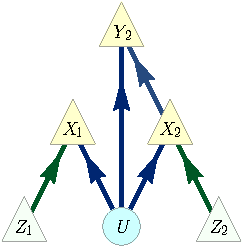
\includegraphics[scale=1]{instrumentalvariant.pdf}
    \caption{An inflation DAG which illustrates why coinciding ancestral subgraphs don't necessarily imply coinciding distributions.}
    \label{fig:ancestralsubgraphnotenough}
    \end{minipage}
\end{figure}

Constraints of the above form be used to supplement the marginal problem, and may be of practical use for reducing the dimensionality of the problem (number of gedankenprobabilities that need to be eliminated by quantifier elimination). However, we are not aware of any case in which this would actually result in tighter exclusions for the distributions on the original DAG. In many cases, this can be explained by the following argument. Suppose that there is an automorphism of the inflation DAG which takes copies of nodes to copies\footnote{Note the similarity to \emph{deck transformations} in covering space theory.} and restricts to an inflationary isomorphism $\ansubgraph[G']{\bm{X}}\sim\ansubgraph[G']{\bm{Y}}$ as above. If $\hat{P}$ solves the unsupplemented marginal problem, then switching the variables in $\hat{P}$ according to the automorphism still solves the unsupplemented marginal problem, since the given marginal distributions are preserved by the automorphism. Now taking the uniform mixture of this new distribution with $\hat{P}$ results in a distribution that still solves the marginal problem, and in addition satisfies the supplemented constraint $P_{\bm{X}} = P_{\bm{Y}}$.

Note that the argument does not apply if there is no automorphism which restricts to $\ansubgraph[G']{\bm{X}}\sim\ansubgraph[G']{\bm{Y}}$, and it also does not apply if one uses the conditional independence relations on the inflation DAG as well, since this destroys linearity. We do not know what happens in either of these cases.

\end{asparadesc}\clearpage







\section{Further Polytope Projection Algorithms}\label{sec:projalgorithms}

Redundant inequalities can be filtered out using Chernikov rules \cite{Shapot2012,Bastrakov2015}. 

% We find the strategy of employing linear programming in concert with the second Cernikov rule to be extremely efficient.

There are plenty of other algorithms for computing the facets of a polytope from its vertices. The Equality Set Projection (ESP) algorithm~\cite{jones2004equality,JonesThesis2005} could be an interesting algorithm to use in practice, as it starts churning out facets one by one from the very beginning, whereas Fourier-Motzkin only has the ability to generate the entire list of facets all in one, which quickly becomes computationally intractable. So ESP may provide a useful tool for deriving an incomplete list of inequalities on inflation DAGs that are too large for the Fourier-Motzkin elimination to work.
% ideal for handling inflation DAGs, because its computational complexity scales only according to the facet count of the final projection. Our use of larger-and-larger inflation DAGs to obtain causal infeasibility criteria on the same underlying original DAG means that while the complexity of the starting polytope is unbounded, the complexity of the projection is finite. Practically, this suggests that the ESP algorithm could parse the implications due to very large inflation DAGs efficiently. Formally, ESP should require minimal computational overhead to consider a larger inflation DAG relative to considering a much smaller inflation DAG, when the \emph{implications} of the small and large inflations are similar. By contrast, the computation complexity of Fourier-Motzkin (FM) elimination algorithm scales with the number of quantifiers being eliminated. The number of gedankenprobabilities requiring elimination is exponentially related to the number of variables in the inflation DAG. The FM algorithm, therefore, is utterly impractical very for large inflation DAGs.

% Another positive feature of the ESP algorithm is that it commences outputting quantifier-free inequalities immediately, and terminates upon deriving the complete set of inequalities. By contrast, FM works by eliminating one quantifier at a time. Terminating the ESP algorithm before it reaches completion would result in an incomplete list of inequalities. Even an incomplete list is valuable, though, since the causal infeasibility criteria we are deriving are anyways necessary but not sufficient.

% Vertex projection (VP) algorithms are another computational tool which may be used to assist in linear quantifier elimination \cite{Avis2000lrs}. VP works by first enumerating the vertices of the initial polytope (H-rep to V-rep), projecting the vertices, and then converting back to inequalities (V-rep to H-rep). For generic high-dimensional polytopes, the operation of converting from a representation in terms of halfspaces to one in terms of extremal-vertices representations can be computationally costly (high-$d$ H-rep to V-rep). Starting from a vertex representation in a high dimensional space, however, one can immediately determine the vertex representation of the polytope's projection in a lower dimensional space. The projection is along the coordinate axes, so one just ``discards" the coordinate of the eliminated quantifier. To obtain the inequalities which characterize the projected polytope one then applies a convex hull algorithm to the projected vertices (low-$d$ V-rep to H-rep).

% For probability distributions, however, the extremal vertices are precisely the deterministic possibilities. Since the extremal vertices of the initial polytope are easily enumerated, it is possible to avoid the high-$d$ V-rep to H-rep step entirely. There is a one-to-one correspondence between the inflation-DAG's initial generating inequalities and its initial extreme observable probability distributions. 
% We used this V-rep to H-rep technique to project the initial marginals-problem polytope implied by \cref{fig:Tri222} to an intermediate 23-dimensional polytope, where the 23 remaining dimensions correspond to the probabilities pertainining to  pre-injectable sets.  Only then did we apply translate those probabilities into probabilities pertaining to the original DAG, and in so doing we convert linear inflation-DAG inequalities to polynomial inequalities pertaining to the original DAG. We found that the V-rep to H-rep technique, using \textit{lrs} [\href[pdfnewwindow]{http://cgm.cs.mcgill.ca/~avis/C/lrslib/USERGUIDE.html#Installation\%20Section}{\texttt{lrs}}], was orders-of-magnitude faster than FM elimination at obtaining the same result.

% Yet another technique is also possible. Suppose the initial polytope is given by $\brackets{\vec{x},\vec{y}\,|\hat{A}.\vec{x}+\hat{B}.\vec{y}\geq\bm{c}}$, where $y$ are the quantifiers. If we can find any completely nonnegative vector $\bm{w}$ such that $\bm{w}.\hat{B}=\vec{0}$ then we automatically establish the quantifier-free inequality $\bm{w}.\hat{A}.\vec{x}\geq\bm{w}.\bm{c}$. Solving for ``random" nonnegative vectors $\bm{w}$ is easy; solving for all possible solutions is rather more difficult. \citet{BalasProjectionCone} refined this method so that each extremal construction of $\bm{w}$ corresponds to an irredundant inequality in the H-rep description of the projected polytope. Nevertheless, even without utilizing the full projection cone, this technique can be used to rapidly obtain a few quantifier-free inequalities. 

%\section{Optimized Algorithm for Recognizing Redundant Inequalities}\label{sec:redundancy}

% When performing Fourier-Motzkin linear quantifier elimination one must periodically filter out redundant inequalities from the set of linear inequalities. Equivalently, the means identifying redundant halfspace constraints in the description of the polytope. An individual constraint in a set is redundant if it is implied by the other constraints. 

% An individual linear inequality is redundant if and only if it is a \emph{positive} linear combination of the others [Thm. 5.8 in \citealp{fordan1999projection}]\footnote{The ``if" is obvious. The ``only if" is a consequence of Farka's lemma \cite{fordan1999projection}.}. This is related to the V-rep characterization of polyhedral cones: If a cone is defined such that $W_{\hat{M}}\coloneqq\brackets{\vec{x}\,|\exists_{\bm{v}\geq\bm{0}}:\, \hat{M}.\bm{v}=\vec{x}}$ then $\vec{b}\in W_{\hat{M}}$ if and only if the linear system of equations $\hat{M}.\bm{v}=\vec{b}$ has a solution such that all the elements of $\bm{v}$ are nonnegative.  Thus, the computational tool required is one which accepts as input the matrix $\hat{M}$ and the column vector $\vec{b}$ and returns $\vec{b}\in W_{\hat{M}}$ as True or False. 


%It turns out that we can optimize the detection of redundant halfspaces when considering polyhedral cones as opposed to polytopes. Happily, the inequalities that pertain to the nonnegativity of probability describe a polytope which is identically the intersection of a cone with a hyperplane. The cone is given by the usual nonnegativity inequalities, just without defining $\p{}=1$. The hyperplane, then, is exactly $\p{}=1$. As the hyperplane-intersection constraint has no bearing on the quantifiers, we can set it aside, perform the projection, and then re-incorporate the $\p{}=1$ normalization condition after the Fourier-Motzkin procedure has completed.

%Consider a polyhedral cone with halfspace representation $W=\brackets{\vec{x}\,|\hat{A}.\vec{x}\geq \bm{0}}$. Each row in $\hat{A}$ is an inequality. Now consider the polar dual of $W$, namely $W^*=\brackets{\vec{x}\,|\exists_{\bm{v}\geq\bm{0}}:\, \hat{A}^{T}.\bm{v}=\vec{x}}$, in extremal-rays representation. Every halfspace (row of $\hat{A}$) in $W$ is associated with a ray (column of $\hat{A}^{T}$) in $W^*$. Critically, though, every irredundant halfspace in $W$ corresponds to an \emph{extremal} ray in $W^*$. Determining if a given ray is extremal or not is a computationally fast task. A ray in $W^*$ is \emph{not} extremal if it \emph{can} be expressed as a \emph{positive} linear combination of the other rays in $W^*$. \purp{Comment about one-to-one if $W$ is convex. Otherwise this trick detects only some, but not all, of the redundant inequalities. Also, citations needed.}

%Thus, the computational tool required is one which accepts as input the matrix $\hat{M}$ and the column vector $\vec{b}$, and which determines if the linear system of equations $\hat{M}.\bm{v}=\vec{b}$ has any solutions such that all the elements of $\bm{v}$ are nonnegative.

%For our purposes, $\hat{M}$ is the set of all rays \emph{other} than $\vec{b}$, where the columns of $\hat{M}$ are the other rays. 

% Below, we present two possible \textit{Mathematica$^{_{\textit{\tiny\texttrademark}}}$} implementations which assess if a given column $\vec{b}$ can be expressed as a positive linear combination of the columns of $\hat{M}$. The former function is easy to understand, but the latter utilizes efficient low-level code and \textit{Mathematica$^{_{\textit{\tiny\texttrademark}}}$}'s internal error-handling to rapidly recognize infeasible linear programs.

\begin{comment}
\begin{align*}
 &\hspace{-\mathindent}\texttt{PositiveLinearSolveTest}[{M}\_?\texttt{MatrixQ},{b}\_]{:=}
 \texttt{With}[\{{vars}=\texttt{Thread}[\texttt{Subscript}[x,{\texttt{Dimensions}[{M}][[2]]}]]\},
 \\&\texttt{Resolve}[
 \texttt{Exists}[\texttt{Evaluate}[{vars}],\;
 \texttt{AllTrue}[{vars},\;\texttt{NonNegative}],
 \\&\texttt{And}\texttt{@@}\texttt{Thread}[{M}.\texttt{vars}==\texttt{Flatten}[{b}]]]]];
%\\\shortintertext{or, using efficient lower-level functions,}
       \\&\hspace{-\mathindent}\text{or}\quad\texttt{PositiveLinearSolveTest}[{M}\_?\texttt{MatrixQ},{b}\_]\texttt{/;Dimensions}[{b}]\texttt{===}\{\texttt{Length}[{M}],1\}{:=}
       \\&\hspace{-6ex}\texttt{Module}[\{{rowcount},{columncount},{fakeobjective},{zeroescolumn}\},
       \\&\hspace{-5ex}\{{rowcount},{columncount}\}=\texttt{Dimensions}[{M}];
       \\&\hspace{-5ex}{fakeobjective}=\texttt{SparseArray}[\{\},\{{columncount}\},0.0];
       \,{zeroescolumn}=\texttt{SparseArray}[\{\},\{{rowcount},1\}];
       \\&\hspace{-5ex}\texttt{Internal$\grave{}$HandlerBlock}[\{\texttt{Message},\texttt{Switch}[\#1,\texttt{Hold}[\texttt{Message}[\texttt{LinearProgramming::lpsnf},\_\_\_],\_],\texttt{Throw}[\texttt{False}]]\texttt{\&}\},
       \\&\texttt{Quiet}[\texttt{Catch}[
       \\&\quad\texttt{LinearProgramming}[{fakeobjective},{M},\texttt{Join}[{b},{zeroescolumn},2],\texttt{Method}\to \texttt{Simplex}];\texttt{True}
       \\&],\{\texttt{LinearProgramming::lpsnf}\}]]];
\end{align*}
To illustrate examples of a when a positive solution to the linear system exists and when it does not, consider the following two examples:.
\begin{align*}
%&\hspace{-\mathindent}
&\texttt{PositiveLinearSolveTest}[
\begin{pmatrix}
 1 & 0 & 1 \\
 0 & 1 & -1 
\end{pmatrix},
\begin{pmatrix}
 1 \\
 -2 
\end{pmatrix}]\;==\;\texttt{False} 
%\quad\text{and}\quad
\\&\texttt{PositiveLinearSolveTest}[
\begin{pmatrix}
 1 & 0 & 1 \\
 0 & 1 & -2 
\end{pmatrix},
\begin{pmatrix}
 1 \\
 -1 
\end{pmatrix}]\;==\;\texttt{True} 
\end{align*}

If $\hat{A}$ is the matrix who's rows are nonnegativity inequalities, then the following test determines if row $n$ is redundant. 
\begin{align*}
 &\hspace{-\mathindent}\texttt{RedundantRowQ}[A\_?\texttt{MatrixQ},n\_\texttt{Integer}]\text{:=}\texttt{PositiveLinearSolveTest@@Reverse}[\texttt{Transpose/@TakeDrop}[A,\{n\}]].
\end{align*}
Note that a \texttt{True} response from \texttt{RedundantRowQ} indicates that the row $n$ is redundant.

%Obtaining a redundancy-free collection of (convex) polyhedral-cone inequalities is therefore related to obtaining a non-negative factorization of a matrix. \purp{Need citation. Also, give explicit connection between NN factorization and redundancy elimination. Does this connection appears elsewhere in the literature?}
\end{comment}

%%% T: I've commented this out since we're not concerned here with observational equivalence, and I have the feeling that it would still require a major clean-up operation. The example of 6 observationally equivalent DAGs is not very good since they are all equivalent to A <-- S --> B, which doesn't contain any latent nodes
\begin{comment}
\clearpage\section{Recognizing observationally equivalent DAGs}

%\purp{Notes to self: Comment about matching-up latent variables between causal structures, for ObsEquiv test.}

%Without loss of generality we herein consider only deterministic DAGs where all latent variables are parentless. \purp{Either prove this, or remove it. If not invoked we should discuss adding edges TO latent variables.}

One expects that an edge $A\to B$ can be added to DAG $G$ while leaving $G$ observationally invariant if the new connection does not introduce any new information about observable variables to $B$. %If the added connection does inform $B$ about some observable $C$, that's still ok so long as the new informational cannot be exploited to increase the correlation between $B$ and $C$.
We can formalize this notion in the language of sufficient statistics. To do so, however, a few background definitions are in order.

\tblue{Perfectly Predictable:} The random variable $X$ is perfectly predictable from a set of variables $\bm{Z}$, hereafter $\mblue{\bm{Z}\vDash X}$, if $X$ can be completely inferred from knowledge of $\bm{Z}$ alone. In a deterministic DAG, for example, every non-root node is perfectly predictable given its parents, ${\NamedFunction{pa}{\!X\!}\vDash X}$. Indeed, in a deterministic DAG the node $X$ is perfectly predictable from $\bm{Z}$ if $X$ is a deterministic descendant of $\bm{Z}$. Operationally, $X$ is a deterministic descendant of $Z$ if the intersection of {[the ancestors of $X$]} with {[the non-ancestors of $Z$]} is a subset of {[the descendants of $Z$]}. Happily though, perfectly predictability can be extrapolated from a causal structure with minimal effort: ${\bm{Z}\vDash X}$ if every directed path to $X$ from any root node is blocked by $\bm{Z}$. 

\tblue{Markov Blanket:} The Markov Blanket for a set of nodes $\bm{V}$, hereafter $\mblue{\NamedFunction{MB}{\!\bm{V}\!}}$, is the set of all of $\bm{V}$'s children, parents, and co-parents. The Markov Blanket is so defined because the nodes in $\bm{V}$ are conditionally independent of \emph{everything} given $\NamedFunction{MB}{\!\bm{V}\!}$. If the random variables in the Markov Blanket $\NamedFunction{MB}{\!\bm{V}\!}$ are known, then information about nodes inside $\bm{V}$ has no bearing on nodes outside the Markov Blanket and vice versa.

\tblue{Markov Partition:} \purp{New! I made this up Nov 24. Useful do you think?} A set of variables $\bm{Z}$ is a Markov Partition for a pair of random variables $X$ and $Y$, hereafter $\mblue{X\cramp{\dashv}\bm{Z}\cramp{\vdash}Y}$, if the pair are conditionally independent of eachother given \emph{any superset} of $\bm{Z}$. Operationally, this means that $X$ and $Y$ are $d$-separated by every superset of $\bm{Z}$. Equivalently, ${X\cramp{\dashv}\bm{Z}\cramp{\vdash}Y}$ if $\NamedFunction{MB}{\!\bm{V}\!}\subseteq \bm{Z}$ and $X\in \bm{V}$ while $Y\not\in \bm{V}$, or if $\NamedFunction{MB}{\!\bm{V}\!}\subseteq \bm{Z}$ and $Y\in \bm{V}$ while $X\not\in \bm{V}$. Happily though, Markov Partitions can be extrapolated from a causal structure with minimal effort: ${X\cramp{\dashv}\bm{Z}\cramp{\vdash}Y}$ if and only if $X$ and $Y$ would be in \emph{disconnected components} under the deletion of all edges initiation from $\bm{Z}$. 

\tblue{Sufficient Statistic:} A set of nodes $\bm{Z}$ is a sufficient statistic for $A$ relative to $X$, hereafter $\mblue{\bm{Z}\vdash A|X}$,
%$\bm{Z}\in\NamedFunction{SS}{\!A|X\!}$, 
if and only if all inferences about $X$ which can be made given knowledge of $A$ are also inferable \emph{without} knowing $A$ but with knowing $\bm{Z}$ instead. In other words, learning $A$ can never teach anything new about $X$ if $\bm{Z}$ is already known. If $X=A$, then the \emph{only way} $\bm{Z}$ can stand in for $A$ when making inferences about $A$ is if $A$ is perfectly predicable given $\bm{Z}$, i.e. ${\bm{Z}\vdash A|A\iff \bm{Z}\vDash A}$. If $A\neq B$ then there are four \purp{and only four?)} ways that $\bm{Z}\vdash A|X$ can be implied by a DAG: If $\bm{Z}\vDash A$, if $\bm{Z}\vDash X$, if $\NamedFunction{MB}{\!\bm{V}\!}\subseteq \bm{Z}$ and $A\in \bm{V}$ while $X\not\in \bm{V}$, or if $\NamedFunction{MB}{\!\bm{V}\!}\subseteq \bm{Z}$ and $X\in \bm{V}$ while $A\not\in \bm{V}$. \purp{Alternatively:} If $A\neq B$ then there are THREE ways that $\bm{Z}\vdash A|X$ can be implied by a DAG: If $\bm{Z}\vDash A$, if $\bm{Z}\vDash X$, and if ${A\cramp{\dashv}\bm{Z}\cramp{\vdash}X}$.

\begin{theorem}\label{theo:edgeadding}
An edge $A\to B$ can be added to $G$ without observational impact if $\NamedFunction{pa}{\!B\!}$ are a sufficient statistic for $A$ relative to all observable nodes, i.e. $\forall_{\text{observable }X}:\NamedFunction{pa}{\!B\!}\vdash A|X$.\\
In particular, the edge $A\to B$ can always be added whenever $\NamedFunction{pa}{\!B\!}\vDash A$, including, but not limited to, the instance  $\NamedFunction{pa}{\!A\!}\subseteq \NamedFunction{pa}{\!B\!}$.\\
Furthermore, the edge $\Lambda\to B$ can be also always be added whenever $\Lambda$ is latent and $\NamedFunction{MB}{\!\Lambda\!}\subseteq\NamedFunction{pa}{\!B\!}$.
\end{theorem}

We can also define an analogous condition for when an edge can be removed from a DAG without impacting it observationally.
\begin{corollary}\label{cor:edgedropping}
An edge $A\to B$ can be dropped from $G$ to form $G'$ such that $G$ and $G'$ are observationally equivalent if \sout{and only if} the edge $A\to B$ can be added (back) to $G'$ while leaving $G'$ observationally invariant per \cref{theo:edgeadding}.
\end{corollary}

On the subject of adding observationally-invariant edges, it is important to recognize when latent nodes can be introduced (or dropped) without observational impact.
\begin{theorem}\label{theo:latentadding}
A (root) latent node $\Lambda$ can be removed from $G$ without observational impact if $\Lambda$ has only one child node and no co-parents ($\Lambda$ is ``equivalent to local randomness"), or if $\Lambda$'s children are also all children of another single latent node ($\Lambda$ is ``covered-for by another latent node"). Conversely, a new root latent node $\Lambda$ can be introduced along with various outgoing edges, without observational impact, if $\Lambda$ would be equivalent to local randomness or covered-for by another latent node.
\end{theorem}

\clearpage
Naturally, two causal structures are observationally equivalent if one can be transformed into the other without observational impact, via \cref{theo:edgeadding,theo:latentadding}. Some examples of observationally equivalent scenarios, and the steps which interconvert them, are given in \cref{fig:equivalences}.
\begin{figure}[hb]
\centering
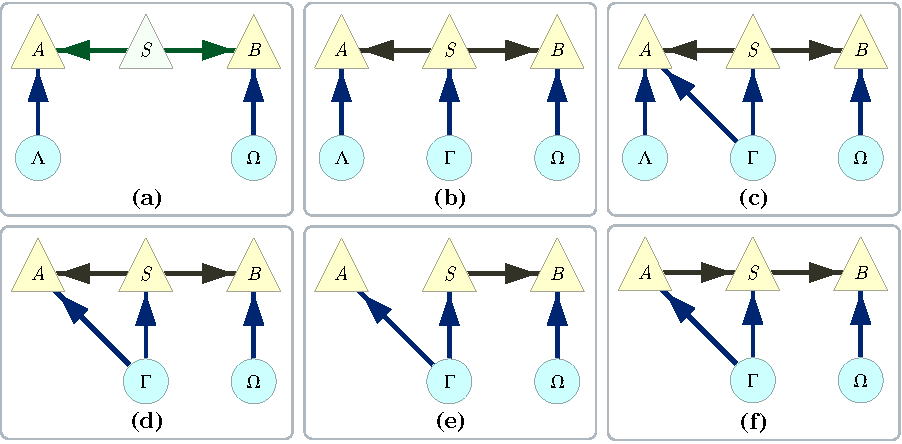
\includegraphics[width=\linewidth]{ObservationalEquivalencesExamples.pdf}
\caption{A set of observational equivalent causal structures. The reasons the changes are observational invariant are as follows: \\
(a)$\sim$(b) because $\Gamma$ is useless in (b), and as such $\Gamma$ can be dropped from (b) per \cref{theo:latentadding}.\\
(b)$\sim$(c) because $\NamedFunction{MB}{\!\Gamma\!}\subseteq\NamedFunction{pa}{\!A\!}$ in (b), and as such $\Gamma\to A$ can be added to (b) per \cref{theo:edgeadding}.\\
(c)$\sim$(d) because $\Lambda$ is redundant to $\Gamma$ in (c), and as such $\Lambda$ can be dropped from (c) per \cref{theo:latentadding}.\\
(d)$\sim$(e) because $\NamedFunction{pa}{\!S\!}\subseteq\NamedFunction{pa}{\!A\!}$ in (e), and as such $S\to A$ can be added to (e) per \cref{theo:edgeadding}.\\
(e)$\sim$(f) because $\NamedFunction{pa}{\!A\!}\subseteq\NamedFunction{pa}{\!S\!}$ in (e), and as such $A\to S$ can be added to (e) per \cref{theo:edgeadding}.
}\label{fig:equivalences}
\end{figure}

%Recall now the two steps of the transformation $\mathsf{ReduceToPCC}$. Imagine after the first step is finished, that an edge $A\to B$ remains, where $A$ is not a root node. Have directly connected all causal pathways, we know that $\NamedFunction{pa}{\!A\!}\subseteq\NamedFunction{pa}{\!B\!}$. As such, $\NamedFunction{pa}{\!B\!}\vDash A$, that is to say, $A$ is perfectly predictable given the parents of $B$. By \cref{theo:edgeadding}, therefore, if the edge $A \to B$ were not in the DAG, we would be able to add that edge without observational impact. By \cref{cor:edgedropping}, therefore, removing that edge has no observational impact. Indeed, the second step of $\mathsf{ReduceToPCC}$ leaves the post-first-step DAG observationally invariant. This allows us to quickly determine if a DAG is PCC-lossless.

%\begin{prop}\label{prop:PCClossless}
%A causal structure $G$ is PCC-lossless if every new edge in $\NamedFunction{ReduceToPCC}{\!G\!}$ relative to $G$ can be accounted for by adding edges to $G$ while leaving $G$ observationally invariant, pursuant to %\cref{theo:edgeadding,theo:latentadding}.
%\end{prop}

%%%%%%%%%%%% Enumeration via lowercase letters
\renewcommand{\labelenumi}{(\alph{enumi})}
\renewcommand{\theenumi}{(\alph{enumi})}
\renewcommand{\labelitemi}{$\circ$}
\end{comment}



\section{The copy lemma and non-Shannon type entropic inequalities}

As it turns out, the inflation DAG technique is also useful outside of the problem of causal inference. As we argue in the following, inflation is secretly what underlies the \tblue{copy lemma} in the derivation of non-Shannon type entropic inequalities~\cite[Chapter~15]{yeung_network_2008}. The following formulation of the copy lemma is the one of Kaced~\cite{kaced_equivalence_2013}.

\begin{lemma}
	Let $A$, $B$ and $C$ be random variables with distribution $P_{ABC}$. Then there exists a fourth random variable $A'$ and joint distribution $P_{AA'BC}$ such that:
	\begin{enumerate}
		\item $P_{AB} = P_{AB'}$,
		\item $A' \perp AC \:|\: B$.
	\label{copylemma}
	\end{enumerate}
\end{lemma}

\begin{figure}[t]
\centering
\begin{minipage}[b]{0.23\linewidth}
\centering
%\includegraphics[scale=1]{}
\caption{A causal structure that is compatible with any distribution $P_{ABC}$.}\label{fig:beforecopy}
\end{minipage}
\hfill
\begin{minipage}[t]{0.38\linewidth}
\centering
%\includegraphics[scale=1]{}
\caption{An inflation.}\label{fig:aftercopy}
\end{minipage}
\end{figure}

\begin{proof}
	Consider the original DAG of~\cref{fig:beforecopy} and the associated inflation DAG of~\cref{fig:aftercopy}. If the original distribution $P_{ABC}$ is compatible with~\cref{fig:beforecopy}, then the associated inflation model marginalizes to a distribution $P_{AA'BC}$ which has the required properties. Hence it remains to be shown that every $P_{ABC}$ is compatible with~\cref{fig:beforecopy}. But this is easy: take $\lambda$ to be any sufficient statistic for the joint variable $(A,B)$ given $C$, such as $\lambda := (A,B,C)$.
\end{proof}

While it is also not hard to write down a distribution with the desired properties explicitly~\cite[Lemma~15.8]{yeung_network_2008}, our purpose of rederiving the lemma via inflation is our hope that more sophisticated applications of the inflation technique will result in \emph{new} non-Shannon type entropic inequalities.


\section{Classifying polynomial inequalities for the Triangle scenario}
\label{sec:38ineqs}

The following polynomial inequalities for the Triangle scenario have been derived via the linear quantifier elimination method of~\cref{sec:ineqs} using the inflation DAG of~\cref{fig:Tri222}. Initially this has resulted in 64 symmetry classes of inequalities, where the symmetries are given by permuting the variables and inverting the outcomes. For the resulting 64 inequalities, numerical checks have found violations of only 38 of them: although they are all facets of the marginal polytope over the distributions on pre-injectable sets, there is no guarantee that they are also nontrivial inequalities at the level of the original DAG, and this has indeed turned out not to be the case for 26 of these symmetry classes of inequalities. Moreover, it is still likely to be the case that some of these inequalities are redundant; we have not yet checked whether for every inequality there is a distribution which violates the inequality but satisfies all others.

In the following table, the inequalities are listed in expectation-value form, where we assume the two possible outcomes of each variables to be $\{-1,+1\}$.

\purp{T: it may be better to list this as a table of coefficients, as e.g.~in \href{http://arxiv.org/abs/1101.2477}{arXiv:1101.2477}, p.14/15?}

\begin{comment}
\begin{align*}\def\arraystretch{1.5} \hspace{-\mathindent}\begin{array}{l}
 0
\leq
{1 + \expec{A B} + \expec{A C} + \expec{B} \expec{C}} \\
 0
\leq
{2 -2 \expec{A C} + \expec{A} \expec{B} \expec{C} -\expec{C} \expec{A B}} \\
 0
\leq
{2 -\expec{A B C} + \expec{C} \expec{A B} + \expec{B} \expec{A C} + \expec{A} \expec{B C}} \\
 0
\leq
{2 + \expec{A B C} + \expec{C} \expec{A B} + \expec{B} \expec{A C} -\expec{A} \expec{B C}} \\
 0
\leq
{3 + \expec{A} + \expec{B} + \expec{C} + 3 \expec{A B} -\expec{A C} -\expec{B} \expec{C} + \expec{A} \expec{B} \expec{C} + \expec{C} \expec{A B} -\expec{B} \expec{A C}} \\
 0
\leq
{3 + \expec{A} + \expec{B} -\expec{C} + 3 \expec{A B} + \expec{A C} + \expec{B} \expec{C} + \expec{A} \expec{B} \expec{C} -\expec{C} \expec{A B} -\expec{B} \expec{A C}} \\
 0
\leq
{3 + \expec{C} -2 \expec{A B} -2 \expec{B C} + \expec{A} \expec{B} + \expec{A} \expec{B} \expec{C} -\expec{C} \expec{A B} -\expec{B} \expec{A C}} \\
 0
\leq
{3 + \expec{B} + \expec{A B} -2 \expec{B C} -\expec{A} \expec{B} + \expec{A} \expec{C} + \expec{A} \expec{B} \expec{C} + \expec{C} \expec{A B} -\expec{B} \expec{A C}} \\
 0
\leq
{3 + \expec{B} + \expec{A B} -2 \expec{B C} + \expec{A} \expec{B} -\expec{A} \expec{C} -\expec{A} \expec{B} \expec{C} + \expec{C} \expec{A B} + \expec{B} \expec{A C}} \\
 0
\leq
{3 -\expec{A} + \expec{B} + \expec{C} -\expec{A B C} + \expec{A} \expec{B} + \expec{A} \expec{C} -\expec{B} \expec{C} + \expec{A} \expec{B} \expec{C} + \expec{C} \expec{A B} + \expec{B} \expec{A C} + \expec{A}
   \expec{B C}} \\
 0
\leq
{3 + \expec{A} + \expec{B} -\expec{C} -2 \expec{A B} + \expec{A B C} + \expec{A} \expec{B} + \expec{A} \expec{C} + \expec{B} \expec{C} + \expec{A} \expec{B} \expec{C} + \expec{C} \expec{A B} + \expec{B} \expec{A C} -\expec{A} \expec{B C}} \\
 0
\leq
{4 + 2 \expec{C} -2 \expec{A B} -2 \expec{A C} -\expec{A B C} + 2 \expec{A} \expec{B} + 2 \expec{B} \expec{C} + \expec{C} \expec{A B} + \expec{B} \expec{A C} + \expec{A} \expec{B C}} \\
 0
\leq
{4 -2 \expec{B} -2 \expec{A B} -3 \expec{B C} + \expec{A B C} + \expec{B} \expec{C} + \expec{A} \expec{B} \expec{C} + \expec{C} \expec{A B} -\expec{B} \expec{A C}} \\
 0
\leq
{4 -2 \expec{C} -2 \expec{A B} -2 \expec{A C} -3 \expec{B C} + \expec{A B C} + 2 \expec{A} \expec{B} + \expec{B} \expec{C} -\expec{A} \expec{B} \expec{C} + \expec{C} \expec{A B} + \expec{B} \expec{A C}} \\
 0
\leq
{4 + 2 \expec{A B} -2 \expec{A C} + \expec{B C} + \expec{A B C} + 2 \expec{A} \expec{B} + 2 \expec{A} \expec{C} -\expec{B} \expec{C} -\expec{A} \expec{B} \expec{C} + \expec{C} \expec{A B} -\expec{B} \expec{A
   C}} \\
 0
\leq
{4 + 2 \expec{A B} -2 \expec{A C} + \expec{B C} + \expec{A B C} -2 \expec{A} \expec{B} + 2 \expec{A} \expec{C} -\expec{B} \expec{C} + \expec{A} \expec{B} \expec{C} + \expec{C} \expec{A B} + \expec{B} \expec{A C}}
   \\
 0
\leq
{4 -2 \expec{A B} + 3 \expec{B C} + \expec{A B C} + 2 \expec{A} \expec{B} + \expec{B} \expec{C} + \expec{A} \expec{B} \expec{C} -\expec{C} \expec{A B} -\expec{B} \expec{A C}} \\
 0
\leq
{4 -2 \expec{B} -2 \expec{A B} + \expec{A B C} -2 \expec{B} \expec{C} + \expec{C} \expec{A B} + \expec{B} \expec{A C} -\expec{A} \expec{B C}} \\
 0
\leq
{4 -2 \expec{A} -2 \expec{A B} -2 \expec{A C} + \expec{A B C} + \expec{C} \expec{A B} + \expec{B} \expec{A C} -\expec{A} \expec{B C}} \\
 0
\leq
{4 -2 \expec{C} -2 \expec{A B} -2 \expec{A C} -2 \expec{B C} + \expec{A B C} + 2 \expec{A} \expec{B} + \expec{C} \expec{A B} + \expec{B} \expec{A C} -\expec{A} \expec{B C}} \\
 0
\leq
{4 -2 \expec{A B} -2 \expec{A C} -2 \expec{B C} + \expec{A B C} + 2 \expec{A} \expec{B} + 2 \expec{A} \expec{C} + 2 \expec{B} \expec{C} + \expec{C} \expec{A B} + \expec{B} \expec{A C} + \expec{A} \expec{B C}} \\
 0
\leq
{5 + \expec{A} + \expec{B} + \expec{C} + 3 \expec{A B} + \expec{A C} -4 \expec{B C} -2 \expec{A} \expec{B} + \expec{B} \expec{C} + \expec{A} \expec{B} \expec{C} + \expec{C} \expec{A B} -\expec{B} \expec{A C}} \\
 0
\leq
{5 + \expec{A} + \expec{B} + \expec{C} + 3 \expec{A B} -\expec{A C} -4 \expec{B C} + 2 \expec{A} \expec{B} -2 \expec{A} \expec{C} + \expec{B} \expec{C} -\expec{A} \expec{B} \expec{C} + \expec{C} \expec{A B} +
   \expec{B} \expec{A C}} \\
 0
\leq
{5 + 3 \expec{A} + \expec{B} + \expec{C} + \expec{A B} + 3 \expec{A C} + \expec{B C} -\expec{A B C} + 2 \expec{A} \expec{B} + 2 \expec{A} \expec{B} \expec{C} -2 \expec{C} \expec{A B}} \\
 0
\leq
{5 + 3 \expec{A} + \expec{B} + \expec{C} + \expec{A B} + 3 \expec{A C} + \expec{B C} -\expec{A B C} + 2 \expec{A} \expec{B} -2 \expec{A} \expec{B} \expec{C} + 2 \expec{C} \expec{A B}} \\
 0
\leq
{6 -3 \expec{A B} -4 \expec{A C} + \expec{A} \expec{B} + 2 \expec{A} \expec{C} + 2 \expec{B} \expec{C} + \expec{A} \expec{B} \expec{C} -\expec{C} \expec{A B} -2 \expec{B} \expec{A C} -2 \expec{A} \expec{B
   C}} \\
 0
\leq
{6 + 2 \expec{B} + 3 \expec{A B} -4 \expec{A C} + \expec{A} \expec{B} + 2 \expec{A} \expec{C} + \expec{A} \expec{B} \expec{C} + \expec{C} \expec{A B} -2 \expec{B} \expec{A C} -2 \expec{A} \expec{B C}} \\
 0
\leq
{6 -2 \expec{A} + 2 \expec{B} -3 \expec{A B} -5 \expec{A C} + \expec{A} \expec{B} + \expec{A} \expec{C} + 2 \expec{A} \expec{B} \expec{C} + \expec{C} \expec{A B} -\expec{B} \expec{A C} -2 \expec{A} \expec{B
   C}} \\
 0
\leq
{6 -3 \expec{A B} + \expec{A C} -2 \expec{B C} + \expec{A} \expec{B} + \expec{A} \expec{C} -4 \expec{B} \expec{C} + 2 \expec{A} \expec{B} \expec{C} + \expec{C} \expec{A B} -\expec{B} \expec{A C} -2 \expec{A}
   \expec{B C}} \\
 0
\leq
{6 + \expec{A B} -3 \expec{A C} + 2 \expec{B C} + \expec{A} \expec{B} + \expec{A} \expec{C} -4 \expec{B} \expec{C} -2 \expec{A} \expec{B} \expec{C} + \expec{C} \expec{A B} -\expec{B} \expec{A C} -2 \expec{A}
   \expec{B C}} \\
 0
\leq
{6 + 2 \expec{C} + 3 \expec{A C} -5 \expec{B C} -2 \expec{A} \expec{B} + \expec{A} \expec{C} + \expec{B} \expec{C} -2 \expec{A} \expec{B} \expec{C} + 2 \expec{C} \expec{A B} + \expec{B} \expec{A C} + \expec{A}
   \expec{B C}} \\
 0
\leq
{6 -3 \expec{A B} -2 \expec{A C} -2 \expec{B C} -2 \expec{A B C} + \expec{A} \expec{B} + 4 \expec{B} \expec{C} + \expec{A} \expec{B} \expec{C} -\expec{C} \expec{A B} -2 \expec{B} \expec{A C}} \\
\end{array}
\end{align*}


\end{comment}
\clearpage
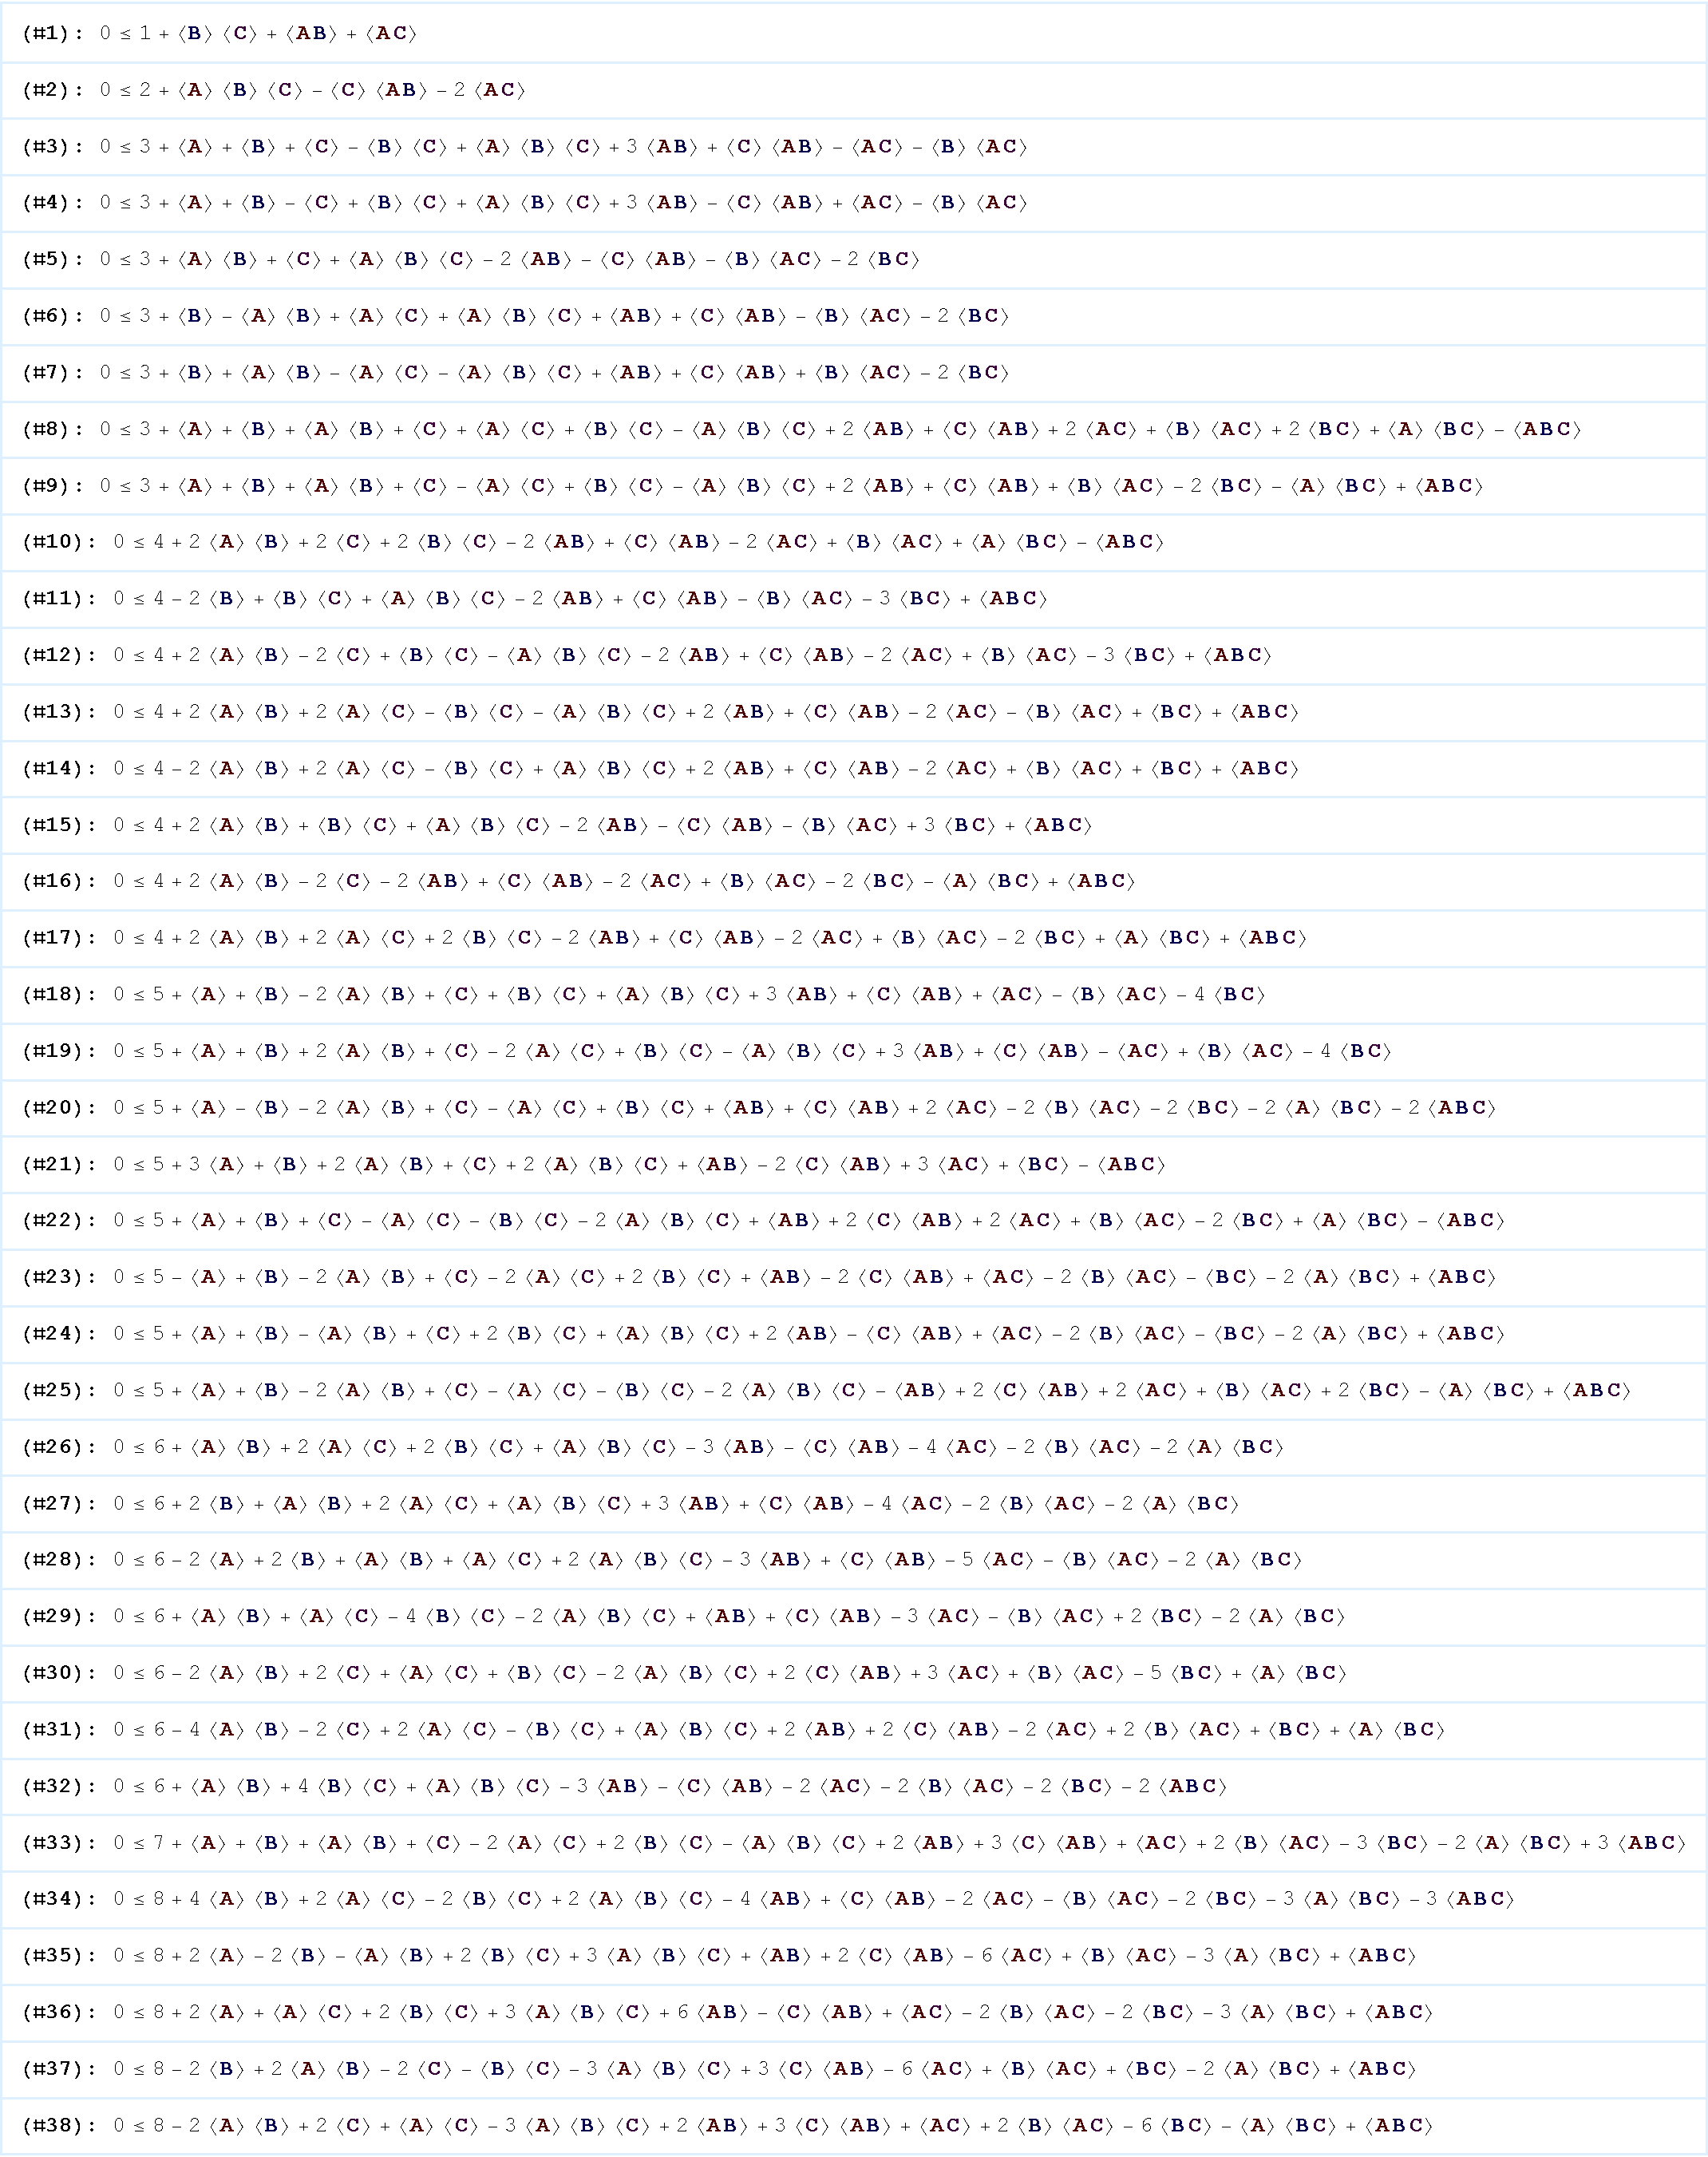
\includepdf[pages=-,scale=0.90]{nontrivlist.pdf}

%\section*{References}
%\nocite{*}
%\setlength{\bibsep}{\smallskipamount}
%\clearpage
\setlength{\bibsep}{3pt plus 3pt minus 2pt}
\bibliographystyle{apsrev4-1}
\nocite{apsrev41Control}
\bibliography{hardyinference}

\end{document}
